% =====================================================================
%  MẪU BÁO CÁO TIỂU LUẬN HỌC PHẦN HỌC MÁY - Nguyễn Tuấn Anh
%  ---------------------------------------------------------------------
%  Biên dịch bằng XeLaTeX (hoặc LuaLaTeX), chạy 2 lần để cập nhật mục lục.
%  Trên Overleaf: Menu > Compiler > XeLaTeX.
%  Trên máy:      latexmk -xelatex "Mau bao cao mon Hoc may.tex"
%
%  Cách dùng mẫu:
%   1. Sửa THÔNG TIN BÁO CÁO ở mục (A) bên dưới.
%   2. Viết nội dung vào các chương; xóa các đoạn \huongdan{...} khi hoàn thành.
%   3. Đặt hình vào thư mục images/ và thay các khung \khunghinh{...}
%      bằng \includegraphics[width=...]{ten_hinh.png}.
% =====================================================================
\documentclass[12pt,a4paper,oneside]{report}

% Cỡ chữ thân bài 13pt (theo quy định trình bày của bộ môn)
\makeatletter
\renewcommand\normalsize{%
  \@setfontsize\normalsize{13pt}{15.6pt}%
  \abovedisplayskip 12pt plus3pt minus7pt
  \belowdisplayskip \abovedisplayskip
  \abovedisplayshortskip 0pt plus3pt
  \belowdisplayshortskip 6.5pt plus3.5pt minus3pt}
\normalsize
\makeatother

% =====================================================================
%  (A) THÔNG TIN BÁO CÁO - SINH VIÊN SỬA TẠI ĐÂY
% =====================================================================
\newcommand{\truong}{TRƯỜNG ĐẠI HỌC CÔNG NGHỆ THÔNG TIN VÀ TRUYỀN THÔNG}
\newcommand{\khoa}{KHOA CÔNG NGHỆ THÔNG TIN}
\newcommand{\loaibaocao}{BÁO CÁO TIỂU LUẬN}
\newcommand{\hocphan}{Học máy}
\newcommand{\lophocphan}{CNTT K22H}
\newcommand{\hocky}{Học kỳ 1, năm học 2026--2027}
\newcommand{\tendetai}{ỨNG DỤNG HỌC MÁY PHÁT HIỆN KHUÔN MẶT NGƯỜI TRONG ẢNH}
\newcommand{\tenbaitoan}{dự đoán kết quả học tập} % dùng trong tên Chương 1 và 2
\newcommand{\giangvien}{Nguyễn Tuấn Anh}  % thêm học hàm/ học vị nếu cần
\newcommand{\nhom}{Nhóm 14}
\newcommand{\svBten}{Trương Công Định}
\newcommand{\svBma}{DTC235200196}
\newcommand{\svAten}{Vũ Anh Đào}
\newcommand{\svAma}{DTC235200171}
\newcommand{\diadiem}{Thái Nguyên}
\newcommand{\thoigian}{tháng 10 năm 2026}

% ---------------- Trang giấy & phông chữ ----------------
\usepackage[a4paper,left=3cm,right=2cm,top=2.5cm,bottom=2.5cm,
            headheight=16pt,headsep=0.8cm]{geometry}
\usepackage{fontspec}
\setmainfont{Times New Roman}
\setmonofont{Courier New}[Scale=0.9]
\usepackage[vietnamese]{babel}
\usepackage{setspace}
\setstretch{1.3}
\setlength{\parindent}{1cm}
\setlength{\parskip}{6pt}
\usepackage{indentfirst}

% ---------------- Gói hỗ trợ ----------------
\usepackage{amsmath,amssymb}
\usepackage{graphicx}
\graphicspath{{images/}}
\usepackage{float}
\usepackage{array,booktabs,tabularx,multirow}
\renewcommand{\arraystretch}{1.25}
\usepackage[table]{xcolor}
\usepackage{tikz}
\usetikzlibrary{positioning,arrows.meta,calc,fit,backgrounds}
\usepackage{caption}
\captionsetup{labelsep=period,labelfont=bf,font=normalsize,skip=6pt}
\captionsetup[table]{position=top}
\usepackage{titlesec}
\usepackage{titletoc}
\usepackage[nottoc]{tocbibind}   % đưa danh mục hình, bảng, TLTK vào mục lục
\usepackage{enumitem}
\setlist{nosep,leftmargin=1.6cm}
\usepackage{listings}
\usepackage{needspace}
\usepackage{cite}                % gộp trích dẫn: [4-6], [2, 4-6]
\usepackage{fancyhdr}
\usepackage[unicode]{hyperref}
\hypersetup{
  hidelinks,
  pdftitle={\tendetai},
  pdfauthor={\svAten, \svBten},
  pdfsubject={\loaibaocao\ học phần \hocphan},
  bookmarksnumbered=true,   % bookmark có số thứ tự chương, mục
  bookmarksopen=true,
  bookmarksopenlevel=0,
}
% Bookmark dạng "Chương 1. Tên chương", "1.1. Tên mục", "Phụ lục A. ..."
\newcommand{\bmchapname}{Chương}
\makeatletter
\newcommand*{\bm@prefix}{}
\let\bm@orig@writebookmark\Hy@writebookmark
\renewcommand*{\Hy@writebookmark}[5]{%
  \ifnum#4=0 \def\bm@prefix{\bmchapname\space}\else\def\bm@prefix{}\fi
  \bm@orig@writebookmark{#1}{#2}{#3}{#4}{#5}}
\renewcommand*{\Hy@numberline}[1]{\bm@prefix#1. }
\makeatother

% ---------------- Màu & định dạng mã nguồn ----------------
\definecolor{codebg}{RGB}{247,247,247}
\definecolor{codekw}{RGB}{0,51,153}
\definecolor{codecm}{RGB}{0,128,0}
\definecolor{codestr}{RGB}{163,21,21}
\definecolor{guide}{RGB}{110,110,110}
\lstdefinestyle{python}{
  language=Python,
  basicstyle=\ttfamily\small\setstretch{1.0},
  backgroundcolor=\color{codebg},
  keywordstyle=\color{codekw}\bfseries,
  commentstyle=\color{codecm}\itshape,
  stringstyle=\color{codestr},
  numbers=left, numberstyle=\tiny\color{guide}, numbersep=8pt,
  frame=single, rulecolor=\color{black!25},
  breaklines=true, showstringspaces=false, tabsize=4,
  xleftmargin=1.2em, framexleftmargin=1.2em,
  aboveskip=8pt, belowskip=8pt, columns=fullflexible, keepspaces=true,
}
\lstset{style=python}
\renewcommand{\lstlistingname}{Đoạn mã}
\renewcommand{\lstlistlistingname}{DANH MỤC ĐOẠN MÃ}

% ---------------- Tên gọi tiếng Việt ----------------
\addto\captionsvietnamese{%
  \renewcommand{\contentsname}{MỤC LỤC}%
  \renewcommand{\listfigurename}{DANH MỤC HÌNH ẢNH}%
  \renewcommand{\listtablename}{DANH MỤC BẢNG}%
  \renewcommand{\bibname}{TÀI LIỆU THAM KHẢO}%
  \renewcommand{\figurename}{Hình}%
  \renewcommand{\tablename}{Bảng}%
  \renewcommand{\chaptername}{Chương}%
  \renewcommand{\appendixname}{Phụ lục}%
}

% ---------------- Đầu trang & chân trang ----------------
\pagestyle{fancy}
\fancyhf{}
\fancyhead[L]{\small\itshape Báo cáo tiểu luận học phần \hocphan}
\fancyhead[R]{\small\itshape\nouppercase{\leftmark}}
\fancyfoot[C]{\thepage}
\renewcommand{\headrulewidth}{0.4pt}
\renewcommand{\chaptermark}[1]{\markboth{\chaptertitlename~\thechapter. #1}{}}
\fancypagestyle{plain}{\fancyhf{}\fancyfoot[C]{\thepage}\renewcommand{\headrulewidth}{0pt}}

% ---------------- Định dạng tiêu đề ----------------
% Chương: "CHƯƠNG 1" + tên chương in hoa - 14pt, đậm, căn giữa
\titleformat{\chapter}[display]
  {\filcenter\bfseries\fontsize{14}{18}\selectfont}
  {\MakeUppercase{\chaptertitlename}~\thechapter}{4pt}{\MakeUppercase}
\titlespacing*{\chapter}{0pt}{0pt}{18pt}
% Mục cấp 2: "1.1. Giới thiệu" - 14pt, đậm
\titleformat{\section}
  {\bfseries\fontsize{14}{18}\selectfont}{\thesection.}{0.5em}{}
\titlespacing*{\section}{0pt}{12pt}{6pt}
% Mục cấp 3: "1.1.1. Mục" - 13pt, đậm
\titleformat{\subsection}
  {\bfseries\fontsize{13}{17}\selectfont}{\thesubsection.}{0.5em}{}
\titlespacing*{\subsection}{0pt}{10pt}{6pt}
% Mục cấp 4: "1.1.1.1. Mục" - 13pt, đậm nghiêng
\setcounter{secnumdepth}{3}
\titleformat{\subsubsection}
  {\bfseries\itshape\fontsize{13}{17}\selectfont}{\thesubsubsection.}{0.5em}{}
\titlespacing*{\subsubsection}{0pt}{8pt}{4pt}

% ---------------- Mục lục & danh mục ----------------
\setcounter{tocdepth}{2}
\newcommand{\tocchapname}{Chương}
\titlecontents{chapter}[0pt]{\addvspace{6pt}\bfseries}
  {\tocchapname~\thecontentslabel.\enspace}{}{\titlerule*[0.6pc]{.}\contentspage}
\titlecontents{section}[1.5em]{}
  {\thecontentslabel.\enspace}{}{\titlerule*[0.6pc]{.}\contentspage}
\titlecontents{subsection}[3em]{}
  {\thecontentslabel.\enspace}{}{\titlerule*[0.6pc]{.}\contentspage}
\titlecontents{figure}[0pt]{}
  {\figurename~\thecontentslabel.\enspace}{}{\titlerule*[0.6pc]{.}\contentspage}
\titlecontents{table}[0pt]{}
  {\tablename~\thecontentslabel.\enspace}{}{\titlerule*[0.6pc]{.}\contentspage}

% ---------------- Lệnh tiện ích ----------------
% Chương không đánh số (Mở đầu, Kết luận...) vẫn có trong mục lục và đầu trang
\newcommand{\unnumberedchapter}[1]{%
  \chapter*{#1}\phantomsection\addcontentsline{toc}{chapter}{#1}\markboth{#1}{}}
% Ghi chú hướng dẫn (xóa khi viết xong)
\newcommand{\huongdan}[1]{{\color{guide}\itshape [Hướng dẫn: #1]}}
% Khung giữ chỗ cho hình: \khunghinh{rộng}{cao}{nội dung}
\newcommand{\khunghinh}[3]{%
  \begin{tikzpicture}
    \draw[dashed,thick,black!40,fill=black!3] (0,0) rectangle (#1,#2);
    \node[text width=0.8*#1,align=center,font=\itshape\color{guide}]
      at ($(0,0)!0.5!(#1,#2)$) {#3};
  \end{tikzpicture}}
% Dòng chấm để viết tay
\newcommand{\dongcham}[1]{\par\noindent\foreach \i in {1,...,#1}{\makebox[\linewidth]{\dotfill}\\[4pt]}}

% =====================================================================
\begin{document}

% =====================================================================
%  TRANG BÌA
% =====================================================================
\begin{titlepage}
  \begin{tikzpicture}[remember picture,overlay]
    \draw[line width=2.2pt]
      ($(current page.north west)+(2.4cm,-1.6cm)$) rectangle
      ($(current page.south east)+(-1.4cm,1.6cm)$);
    \draw[line width=0.6pt]
      ($(current page.north west)+(2.55cm,-1.75cm)$) rectangle
      ($(current page.south east)+(-1.55cm,1.75cm)$);
  \end{tikzpicture}\par\vspace*{-\baselineskip}
  \centering\setstretch{1.2}
  {\fontsize{13}{18}\selectfont\bfseries \truong\par}
  {\fontsize{14}{18}\selectfont\bfseries \khoa\par}
  \vspace{2pt}\rule{0.35\textwidth}{0.8pt}\par
  \vspace{1.2cm}
  \IfFileExists{images/logo.jpg}
    {
\includegraphics[width=3.2cm]{logo.jpg}}
    {\khunghinh{3.2cm}{3.2cm}{Logo\\trường}}\par
  \vspace{1.2cm}
  {\fontsize{22}{28}\selectfont\bfseries \loaibaocao\par}
  \vspace{4pt}
  {\fontsize{16}{20}\selectfont\bfseries HỌC PHẦN: \MakeUppercase{\hocphan}\par}
  \vspace{1.2cm}
  {\fontsize{14}{18}\selectfont ĐỀ TÀI:\par}
  \vspace{4pt}
  {\fontsize{18}{26}\selectfont\bfseries \tendetai\par}
  \vfill
  \begin{tabular}{@{}l@{\hspace{0.6cm}}l@{}}
    \textbf{Giảng viên hướng dẫn:} & \giangvien \\
    \textbf{Lớp học phần:}         & \lophocphan \\
    \textbf{Nhóm thực hiện:}       & \nhom \\
                                   & \svBten\ -- \svBma \\
                                   & \svAten\ -- \svAma \\
  \end{tabular}\par
  \vspace{1.8cm}
  {\bfseries \diadiem, \thoigian\par}
\end{titlepage}

% =====================================================================
%  PHẦN ĐẦU (đánh số trang La Mã)
% =====================================================================
\pagenumbering{roman}
\pagestyle{plain}

% ---------------- Nhận xét của giảng viên ----------------
\chapter*{NHẬN XÉT CỦA GIẢNG VIÊN}
\noindent\textbf{1. Về hình thức và bố cục báo cáo:}
\dongcham{3}
\noindent\textbf{2. Về nội dung và kết quả thực hiện:}
\dongcham{5}
\noindent\textbf{3. Về tinh thần, thái độ làm việc của nhóm:}
\dongcham{3}
\noindent\textbf{4. Điểm đánh giá:}
\begin{center}
  \begin{tabular}{|>{\centering\arraybackslash}p{1.2cm}|p{5.5cm}|>{\centering\arraybackslash}p{2.6cm}|>{\centering\arraybackslash}p{2.6cm}|}
    \hline
    \rowcolor{black!8}\textbf{STT} & \textbf{Họ và tên sinh viên} & \textbf{Điểm số} & \textbf{Điểm chữ} \\ \hline
    1 & \svAten & & \\ \hline
    2 & \svBten & & \\ \hline
  \end{tabular}
\end{center}
\vspace{0.6cm}
\hfill
\begin{minipage}{0.45\textwidth}
  \centering
  \textit{\diadiem, ngày \dots\ tháng \dots\ năm \dots}\\
  \textbf{Giảng viên}\\
  \textit{(Ký và ghi rõ họ tên)}\\[1.8cm]
  \giangvien
\end{minipage}

% ---------------- Lời cam đoan ----------------
\unnumberedchapter{LỜI CAM ĐOAN}

Chúng em xin cam đoan báo cáo tiểu luận ``\textit{\tendetai}'' là kết quả
làm việc của nhóm dưới sự hướng dẫn của giảng viên \giangvien. Các số liệu,
kết quả thực nghiệm trình bày trong báo cáo là trung thực, được tạo ra từ
mã nguồn của nhóm và có thể chạy lại được. Mọi tài liệu, mã nguồn, dữ liệu
tham khảo đều được trích dẫn đầy đủ trong danh mục tài liệu tham khảo.

\textbf{Khai báo sử dụng công cụ AI tạo sinh.}
{Nhóm có sử dụng các công cụ AI tạo sinh ChatGPT và Gemini trong quá trình thực hiện đề tài nhằm hỗ trợ tìm hiểu kiến thức, nghiên cứu và tham khảo tài liệu liên quan. Bên cạnh đó, nhóm sử dụng công cụ Antigravity để hỗ trợ viết, chỉnh sửa và hoàn thiện mã nguồn. Các nội dung, mã nguồn và kết quả do công cụ hỗ trợ tạo ra đều được nhóm xem xét, kiểm tra và điều chỉnh trong quá trình thực hiện.}

Nếu phát hiện có bất kỳ sự gian lận nào, chúng em xin hoàn toàn chịu trách
nhiệm trước giảng viên và nhà trường.

\vspace{0.6cm}
\hfill
\begin{minipage}{0.5\textwidth}
  \centering
  \textit{\diadiem, ngày \dots\ tháng \dots\ năm \dots}\\
  \textbf{Nhóm sinh viên thực hiện}\\
  \textit{(Ký và ghi rõ họ tên)}\\[2cm]
  \begin{tabular}{@{}c@{\hspace{1.5cm}}c@{}}
    \svAten & \svBten
  \end{tabular}
\end{minipage}

% ---------------- Lời cảm ơn ----------------
\unnumberedchapter{LỜI CẢM ƠN}

{Trước hết, chúng em xin gửi lời cảm ơn chân thành và sâu sắc đến giảng viên Nguyễn Tuấn Anh, người đã tận tình giảng dạy, hướng dẫn và truyền đạt những kiến thức quý báu trong suốt quá trình học tập học phần Học máy. Những kiến thức và sự hướng dẫn của thầy đã giúp chúng em có nền tảng lý thuyết và phương pháp thực hành để nghiên cứu, xây dựng và thực hiện đề tài “Phát hiện khuôn mặt người trong ảnh”.

Chúng em xin chân thành cảm ơn thầy đã tạo điều kiện thuận lợi, giải đáp những thắc mắc và đưa ra những định hướng trong quá trình thực hiện đề tài. Đồng thời, chúng em cũng xin cảm ơn các tổ chức và cộng đồng nghiên cứu đã công khai những bộ dữ liệu, tài liệu tham khảo và thư viện mã nguồn mở, đặc biệt là bộ dữ liệu Labeled Faces in the Wild (LFW), góp phần hỗ trợ quá trình tìm hiểu, xây dựng, huấn luyện và đánh giá các mô hình học máy.

Trong quá trình thực hiện đề tài, chúng em đã gặp một số khó khăn trong việc thu thập và xử lý dữ liệu ảnh, tìm hiểu nguyên lý các thuật toán học máy, xây dựng mô hình và đánh giá kết quả thực nghiệm. Tuy nhiên, thông qua quá trình tự nghiên cứu, thực hành và vận dụng những kiến thức đã được học, chúng em đã có cơ hội củng cố kiến thức chuyên môn, nâng cao kỹ năng lập trình Python, khả năng phân tích dữ liệu và hiểu rõ hơn về quy trình xây dựng một hệ thống học máy.

Mặc dù đã cố gắng hoàn thành đề tài một cách tốt nhất, nhưng do kiến thức và kinh nghiệm thực tiễn còn hạn chế, báo cáo khó tránh khỏi những thiếu sót. Chúng em rất mong nhận được những ý kiến nhận xét và góp ý từ thầy để có thể tiếp tục hoàn thiện, nâng cao chất lượng và phát triển đề tài trong tương lai.

Chúng em xin chân thành cảm ơn!}

\vspace{0.4cm}
\hfill
\begin{minipage}{0.58\textwidth}
  \centering
  \textit{Nhóm sinh viên thực hiện}\\[0.8cm]
  \begin{tabular}{@{}c@{\hspace{0.8cm}}c@{}}
    \svAten & \svBten
  \end{tabular}
\end{minipage}

% ---------------- Bảng phân công ----------------
\unnumberedchapter{BẢNG PHÂN CÔNG NHIỆM VỤ}

\begin{center}
\begin{tabularx}{\textwidth}{|>{\centering\arraybackslash}p{1cm}|p{3.4cm}|X|>{\centering\arraybackslash}p{2.5cm}|}
  \hline
  \rowcolor{black!8}\textbf{STT} & \textbf{Họ và tên} & \textbf{Nhiệm vụ phụ trách} & \textbf{Mức độ hoàn thành} \\ \hline
  1 & \svAten\newline \svAma &
    -- Khảo sát, tiền xử lý dữ liệu (Chương 3)\newline
    -- Xây dựng mô hình \dots\ (Chương 2)\newline
    -- Viết báo cáo các mục \dots & 100\% \\ \hline
  2 & \svBten\newline \svBma &
    -- Phân tích tương quan đặc trưng (Chương 3)\newline
    -- Tối ưu siêu tham số (Chương 3)\newline
    -- Xây dựng chương trình demo & 100\% \\ \hline
\end{tabularx}
\end{center}

% ---------------- Mục lục, danh mục ----------------
\begingroup\setstretch{1.1}\tableofcontents\endgroup
\listoffigures
\listoftables

% ---------------- Danh mục từ viết tắt ----------------
\unnumberedchapter{DANH MỤC TỪ VIẾT TẮT}

\begin{center}
\begin{tabularx}{\textwidth}{|>{\centering\arraybackslash}p{1cm}|p{2.6cm}|X|}
  \hline
  \rowcolor{black!8}\textbf{STT} & \textbf{Viết tắt} & \textbf{Ý nghĩa} \\ \hline
  1 & AdaBoost & Adaptive Boosting -- Thuật toán tăng cường thích nghi \\ \hline
  2 & AI & Artificial Intelligence -- Trí tuệ nhân tạo \\ \hline
  3 & AUC & Area Under the Curve -- Diện tích dưới đường cong \\ \hline
  4 & CV & Computer Vision -- Thị giác máy tính \\ \hline
  5 & DR & Detection Rate -- Tỷ lệ phát hiện \\ \hline
  6 & FN & False Negative -- Âm tính giả \\ \hline
  7 & FP & False Positive -- Dương tính giả \\ \hline
  8 & FPR & False Positive Rate -- Tỷ lệ dương tính giả \\ \hline
  9 & LFW & Labeled Faces in the Wild -- Bộ dữ liệu khuôn mặt trong môi trường tự nhiên \\ \hline
  10 & ML & Machine Learning -- Học máy \\ \hline
  11 & ROC & Receiver Operating Characteristic -- Đường đặc tính hoạt động của bộ phân loại \\ \hline
  12 & ROC-AUC & Area Under the ROC Curve -- Diện tích dưới đường cong ROC \\ \hline
  13 & SVM & Support Vector Machine -- Máy vectơ hỗ trợ \\ \hline
  14 & TN & True Negative -- Âm tính thật \\ \hline
  15 & TP & True Positive -- Dương tính thật \\ \hline
  16 & VJ & Viola--Jones -- Phương pháp phát hiện khuôn mặt Viola--Jones \\ \hline
\end{tabularx}
\end{center}


% =====================================================================
%  PHẦN NỘI DUNG (đánh số trang Ả Rập)
% =====================================================================
\clearpage
\pagenumbering{arabic}
\pagestyle{fancy}

% =====================================================================
%  MỞ ĐẦU
% =====================================================================
\unnumberedchapter{MỞ ĐẦU}

\section*{1. Lý do chọn đề tài}
{Trong những năm gần đây, trí tuệ nhân tạo và thị giác máy tính ngày càng được ứng dụng rộng rãi trong nhiều lĩnh vực như giám sát an ninh, nhận dạng khuôn mặt, điểm danh tự động và xử lý hình ảnh. Trong đó, phát hiện khuôn mặt người trong ảnh là một bài toán quan trọng, đóng vai trò nền tảng cho nhiều hệ thống thông minh.

Tuy nhiên, việc phát hiện khuôn mặt vẫn gặp nhiều khó khăn do sự thay đổi về ánh sáng, góc nhìn, kích thước khuôn mặt và bối cảnh hình ảnh. Vì vậy, việc nghiên cứu các thuật toán học máy nhằm nâng cao khả năng phát hiện và giảm thời gian xử lý là cần thiết.

Thuật toán AdaBoost kết hợp với phương pháp Viola–Jones, sử dụng đặc trưng Haar-like, ảnh tích phân và bộ phân loại tầng, là một hướng tiếp cận tiêu biểu trong phát hiện khuôn mặt. Phương pháp này có ý nghĩa khoa học trong việc nghiên cứu học máy tổ hợp, lựa chọn đặc trưng và tối ưu hóa quá trình phân loại; đồng thời có giá trị thực tiễn trong xây dựng các ứng dụng xử lý ảnh.

Xuất phát từ những lý do trên, nhóm lựa chọn đề tài “Phát hiện khuôn mặt người trong ảnh” nhằm tìm hiểu nguyên lý của các thuật toán học máy và vận dụng vào xây dựng hệ thống phát hiện khuôn mặt trên ảnh thực tế.}

\section*{2. Mục tiêu và nhiệm vụ}
{ 2.1. Mục tiêu tổng quát

Nghiên cứu và xây dựng hệ thống phát hiện khuôn mặt người trong ảnh dựa trên thuật toán AdaBoost kết hợp với đặc trưng Haar-like và phương pháp Viola–Jones. Hệ thống hướng đến khả năng phân biệt vùng ảnh chứa khuôn mặt và không chứa khuôn mặt, đồng thời xác định vị trí khuôn mặt trên ảnh đầu vào.

2.2. Mục tiêu cụ thể

Nghiên cứu nguyên lý Boosting, AdaBoost, đặc trưng Haar-like, ảnh tích phân và bộ phân loại tầng Viola–Jones.

Xây dựng bộ dữ liệu dự kiến khoảng 3.000–4.000 ảnh gồm hai lớp khuôn mặt và không phải khuôn mặt, được chuyển về ảnh xám kích thước 24×24 pixel.

Thực hiện khảo sát, tiền xử lý dữ liệu, trích xuất đặc trưng Haar-like và phân tích mối quan hệ giữa đặc trưng với nhãn.

Cài đặt AdaBoost với Decision Stump bằng NumPy và đối chiếu với AdaBoostClassifier của Scikit-learn; xây dựng bộ phân loại tầng đơn giản gồm 2–3 tầng.

Khảo sát ảnh hưởng của số vòng Boosting, Learning Rate và số lượng đặc trưng. Đánh giá mô hình bằng Detection Rate, False Positive Rate, ROC-AUC và thời gian xử lý.

Áp dụng cửa sổ trượt đa tỷ lệ để phát hiện khuôn mặt trên ảnh thực và so sánh với Haar Cascade của OpenCV.

2.3. Nhiệm vụ thực hiện

Nhóm tiến hành nghiên cứu tài liệu; thu thập và tiền xử lý dữ liệu; khảo sát thống kê và chất lượng dữ liệu; xây dựng chương trình trích xuất đặc trưng và huấn luyện mô hình; thực hiện các thí nghiệm, đánh giá, so sánh kết quả và hoàn thiện báo cáo.}

\section*{3. Đối tượng và phạm vi nghiên cứu}
{3.1. Đối tượng nghiên cứu

Đối tượng nghiên cứu là bài toán phát hiện khuôn mặt người trong ảnh số, tập dữ liệu ảnh khuôn mặt(face) và không phải khuôn mặt(non-face), các đặc trưng Haar-like, thuật toán AdaBoost và phương pháp phân loại tầng Viola–Jones.

3.2. Phạm vi nghiên cứu

Về dữ liệu: Sử dụng ảnh khuôn mặt từ LFW hoặc nguồn phù hợp và ảnh không chứa khuôn mặt được thu thập từ ảnh nền. Các mẫu được xử lý thành ảnh xám kích thước 24×24 pixel.

Về nội dung: Tập trung nghiên cứu, cài đặt và đánh giá AdaBoost kết hợp Haar-like và bộ phân loại tầng để phát hiện khuôn mặt. Không đi sâu vào nhận dạng danh tính, tuổi tác hoặc biểu cảm.

Về thời gian: Thực hiện trong học kỳ I, năm học 2026–2027, theo các giai đoạn khảo sát dữ liệu, xây dựng mô hình và đánh giá kết quả.

Về môi trường: Triển khai trên máy tính cá nhân bằng Python và các thư viện học máy, tập trung vào ảnh tĩnh, ưu tiên khuôn mặt nhìn tương đối trực diện.}

\section*{4. Phương pháp thực hiện}
{Đề tài kết hợp nghiên cứu lý thuyết với lập trình và thực nghiệm theo các bước sau:

Bước 1. Nghiên cứu lý thuyết: Tìm hiểu Boosting, AdaBoost, Decision Stump, đặc trưng Haar-like, ảnh tích phân và cấu trúc Cascade của phương pháp Viola–Jones.

Bước 2. Thu thập và tiền xử lý dữ liệu: Thu thập ảnh khuôn mặt và ảnh nền, chuyển ảnh sang mức xám, thay đổi kích thước về 24×24 pixel, gán nhãn và kiểm tra chất lượng dữ liệu. Khảo sát thống kê, phân bố nhãn, mối quan hệ giữa các đặc trưng; xử lý dữ liệu trùng lặp, bất thường và chia tập huấn luyện, xác thực, kiểm tra theo nguyên tắc hạn chế rò rỉ dữ liệu.

Bước 3. Trích xuất đặc trưng: Sử dụng ảnh tích phân để tính toán các đặc trưng Haar-like, tạo vector đặc trưng làm đầu vào cho mô hình học máy.

Bước 4. Xây dựng mô hình: Cài đặt AdaBoost bằng NumPy, đối chiếu với Scikit-learn và xây dựng bộ phân loại tầng đơn giản gồm 2–3 tầng.

Bước 5. Đánh giá và ứng dụng: Khảo sát các tham số mô hình, đánh giá bằng Detection Rate, False Positive Rate, ROC-AUC và thời gian xử lý. Áp dụng cửa sổ trượt đa tỷ lệ để phát hiện khuôn mặt trên ảnh thực tế, sau đó so sánh với Haar Cascade của OpenCV.

Công cụ sử dụng: Python, Anaconda, Jupyter Notebook, NumPy, Pandas, Scikit-learn, OpenCV, Matplotlib, Seaborn và LaTeX (Overleaf) để lập trình, phân tích dữ liệu, trực quan hóa và trình bày báo cáo.\dots).}

\section*{5. Bố cục báo cáo}
Ngoài phần Mở đầu, Kết luận, Tài liệu tham khảo và Phụ lục, báo cáo gồm
3 chương:
\begin{itemize}
  \item \textbf{Chương 1. Tổng quan về học máy và bài toán phát hiện khuôn mặt người trong ảnh:} trình bày bài toán,
        các công trình liên quan và cơ sở lý thuyết của các thuật toán sử dụng.
  \item \textbf{Chương 2. Mô hình hóa bài toán và phương pháp \tenbaitoan:} phát biểu bài
        toán, mục tiêu, lựa chọn thuật toán, mô hình cơ sở, quy trình huấn
        luyện và phương pháp đánh giá.
  \item \textbf{Chương 3. Thực nghiệm và đánh giá:} dữ liệu thực nghiệm (mô
        tả, khảo sát, tiền xử lý), kết quả huấn luyện, phân tích, tối ưu và
        cải tiến, lựa chọn mô hình cuối cùng.
\end{itemize}

% =====================================================================
%  CHƯƠNG 1
% =====================================================================
\chapter{Tổng quan về học máy và bài toán HỌC MÁY PHÁT HIỆN KHUÔN MẶT
NGƯỜI TRONG ẢNH}
\label{chap:tongquan}

\section{Giới thiệu bài toán }
{Phát hiện khuôn mặt người trong ảnh là một bài toán quan trọng trong lĩnh vực thị giác máy tính và học máy, được ứng dụng rộng rãi trong các hệ thống giám sát an ninh, điểm danh tự động, nhận dạng khuôn mặt và xử lý hình ảnh. Mục tiêu của bài toán là xác định sự xuất hiện và vị trí của một hoặc nhiều khuôn mặt trong ảnh đầu vào.

Trong thực tế, việc phát hiện khuôn mặt gặp nhiều khó khăn do sự thay đổi về kích thước, góc nhìn, điều kiện ánh sáng và bối cảnh hình ảnh. Để giải quyết vấn đề này, đề tài nghiên cứu thuật toán AdaBoost kết hợp với đặc trưng Haar-like, ảnh tích phân và phương pháp phân loại tầng Viola–Jones nhằm phân biệt các vùng ảnh chứa khuôn mặt và không chứa khuôn mặt.

Kết quả nghiên cứu hướng đến xây dựng chương trình có khả năng tự động phát hiện và đánh dấu vị trí khuôn mặt trên ảnh, hỗ trợ các ứng dụng xử lý ảnh và hệ thống nhận dạng thông minh. Đồng thời, đề tài giúp làm rõ quy trình xây dựng một hệ thống học máy, từ thu thập, tiền xử lý dữ liệu đến huấn luyện và đánh giá mô hình.}

Quy trình thực hiện dự án học máy của nhóm được mô tả tổng quát trong
Hình~\ref{fig:quytrinh}.

\begin{figure}[H]
  \centering
  \resizebox{\linewidth}{!}{%
  \begin{tikzpicture}[
      node distance=0.35cm,
      buoc/.style={draw,rounded corners=3pt,fill=black!5,minimum height=1.2cm,
                   text width=1.85cm,align=center,font=\small},
      mui/.style={-{Stealth[length=2.5mm]},thick}]
    
    % Hàng trên: Luồng tuần tự
    \node[buoc] (b1) {Phát biểu\\bài toán};
    \node[buoc,right=of b1] (b2) {Thu thập\\dữ liệu ảnh};
    \node[buoc,right=of b2] (b3) {Khảo sát \&\\tiền xử lý};
    \node[buoc,right=of b3] (b4) {Trích xuất\\đặc trưng};
    \node[buoc,right=of b4] (b5) {Huấn luyện\\mô hình};
    \node[buoc,right=of b5] (b6) {Đánh giá\\mô hình};
    
    % Hàng dưới: Vòng lặp cải tiến và triển khai
    \node[buoc,below=0.9cm of b5] (b7) {Tối ưu \&\\cải tiến};
    \node[buoc,below=0.9cm of b2] (b8) {Triển khai\\(demo)};
    
    % Các đường nối mũi tên
    \draw[mui] (b1) -- (b2);
    \draw[mui] (b2) -- (b3);
    \draw[mui] (b3) -- (b4);
    \draw[mui] (b4) -- (b5);
    \draw[mui] (b5) -- (b6);
    \draw[mui] (b6) |- (b7);
    \draw[mui] (b7) -- (b5);
    \draw[mui] (b7) -- (b8);
  \end{tikzpicture}%
  }
  \caption{Quy trình thực hiện dự án học máy}
  \label{fig:quytrinh}
\end{figure}

\section{Các công trình nghiên cứu liên quan}
{Bài toán phát hiện khuôn mặt đã được nghiên cứu rộng rãi với nhiều phương pháp học máy và thị giác máy tính, từ các thuật toán truyền thống đến mô hình học sâu.

Viola và Jones (2001) [1] đề xuất phương pháp phát hiện khuôn mặt kết hợp đặc trưng Haar-like, ảnh tích phân, AdaBoost và bộ phân loại tầng (Cascade). Phương pháp đạt tốc độ xử lý cao trên bộ dữ liệu MIT+CMU nhưng còn hạn chế với khuôn mặt nghiêng và điều kiện ánh sáng phức tạp.

Lienhart và Maydt (2002) [2] mở rộng tập đặc trưng Haar-like bằng các đặc trưng xoay 45°, giúp cải thiện khả năng phát hiện và giảm tỷ lệ cảnh báo sai. Tuy nhiên, việc mở rộng đặc trưng làm tăng độ phức tạp trong quá trình huấn luyện.

Zhang và cộng sự (2016) [3] phát triển MTCNN, sử dụng mạng nơ-ron tích chập nhiều tầng để phát hiện và định vị các điểm đặc trưng khuôn mặt, đạt hiệu quả tốt trên FDDB và WIDER FACE nhưng đòi hỏi quy trình huấn luyện phức tạp hơn.

Deng và cộng sự (2020) [4] đề xuất RetinaFace, ứng dụng học sâu để phát hiện khuôn mặt đa tỷ lệ, đạt độ chính xác cao trên WIDER FACE nhưng yêu cầu tài nguyên tính toán đáng kể.

Từ các nghiên cứu trên, nhóm lựa chọn AdaBoost và Viola–Jones làm phương pháp nghiên cứu chính. Đề tài tập trung tự cài đặt AdaBoost bằng NumPy, trích xuất đặc trưng Haar-like, xây dựng bộ phân loại tầng đơn giản và so sánh với Haar Cascade của OpenCV nhằm đánh giá hiệu quả phát hiện và thời gian xử lý.}

\section{Cơ sở lý thuyết các thuật toán sử dụng}
\subsection{Thuật toán 1: Hồi quy Logistic}
Hồi quy Logistic ước lượng xác suất một mẫu $\mathbf{x}$ thuộc lớp dương
thông qua hàm sigmoid:
\begin{equation}
  P(y=1 \mid \mathbf{x}) = \sigma(\mathbf{w}^{\top}\mathbf{x}+b)
  = \frac{1}{1+e^{-(\mathbf{w}^{\top}\mathbf{x}+b)}}.
  \label{eq:sigmoid}
\end{equation}

\subsection{Thuật toán 2: Rừng ngẫu nhiên}
Rừng ngẫu nhiên \cite{breiman2001} kết hợp nhiều cây quyết định được huấn
luyện trên các mẫu bootstrap và tập con đặc trưng ngẫu nhiên\dots

\subsection{Thuật toán 3: XGBoost}
XGBoost \cite{chen2016} là thuật toán tăng cường độ dốc (gradient boosting)
trên cây quyết định\dots

\section{Các chỉ số đánh giá mô hình}
Trong bài toán phân loại ảnh con, lớp dương được quy ước
là khuôn mặt và lớp âm là không phải khuôn mặt.
Các thành phần của ma trận nhầm lẫn gồm:

\begin{itemize}
    \item $TP$: số ảnh khuôn mặt được phân loại đúng là face.
    \item $FN$: số ảnh khuôn mặt bị phân loại thành non-face.
    \item $FP$: số ảnh nền bị phân loại nhầm thành face.
    \item $TN$: số ảnh nền được phân loại đúng là non-face.
\end{itemize}

Tỷ lệ phát hiện đúng khuôn mặt (Detection Rate):
\begin{equation}
    \mathrm{DR} = \frac{TP}{TP+FN}.
    \label{eq:dr}
\end{equation}

Tỷ lệ dương tính giả (False Positive Rate):
\begin{equation}
    \mathrm{FPR} = \frac{FP}{FP+TN}.
    \label{eq:fpr}
\end{equation}

DR phản ánh tỷ lệ nhận đúng trong các ảnh khuôn mặt thật,
còn FPR phản ánh tỷ lệ báo nhầm trong các ảnh nền thật.
Hai chỉ số được đánh giá tại cùng một ngưỡng phân loại.
Mục tiêu là đạt DR cao đồng thời duy trì FPR thấp.

Đường ROC biểu diễn DR theo FPR khi thay đổi ngưỡng
phân loại. ROC-AUC là diện tích dưới đường ROC,
tóm tắt khả năng phân biệt hai lớp qua nhiều ngưỡng.

Thời gian xử lý được báo cáo theo đơn vị mili giây
trên mỗi ảnh, kèm cấu hình máy, kích thước ảnh và
các bước được tính thời gian.

\section{Kết luận chương 1}
{Chương 1 đã trình bày tổng quan về bài toán phát hiện khuôn mặt người trong ảnh, các ứng dụng thực tiễn và những thách thức trong quá trình phát hiện. Đồng thời, chương đã khảo sát các công trình nghiên cứu liên quan, làm cơ sở cho việc lựa chọn thuật toán AdaBoost kết hợp với phương pháp Viola–Jones. Các kiến thức nền tảng về đặc trưng Haar-like, ảnh tích phân, bộ phân loại tầng và các chỉ số đánh giá như Detection Rate, False Positive Rate, ROC-AUC và thời gian xử lý cũng được đề cập nhằm định hướng quá trình xây dựng mô hình.

Trên cơ sở lý thuyết đã nghiên cứu, Chương 2 sẽ tập trung vào việc mô hình hóa bài toán, xác định đầu vào và đầu ra, lựa chọn phương pháp trích xuất đặc trưng, xây dựng mô hình và thiết kế quy trình huấn luyện, đánh giá phù hợp.}

% =====================================================================
%  CHƯƠNG 2
% =====================================================================
\chapter{Mô hình hóa bài toán và phương pháp \tenbaitoan}
\label{chap:phuongphap}


\section{Phát biểu bài toán học máy}

Đề tài ``Phát hiện khuôn mặt người trong ảnh'' hướng đến việc
xác định sự xuất hiện và vị trí của khuôn mặt trong ảnh.
Hệ thống dự kiến sử dụng bộ phân loại ảnh con kết hợp với
cửa sổ trượt đa tỷ lệ. Bài toán được phát biểu như sau:

\begin{itemize}
    \item \textbf{Loại bài toán:}
    Ở mức ảnh đầy đủ, đây là bài toán phát hiện đối tượng.
    Thành phần học máy cốt lõi ở mức ảnh con là phân loại
    nhị phân có giám sát, phân biệt hai lớp: khuôn mặt
    (face) và không phải khuôn mặt (non-face).
    Khi huấn luyện, mỗi mẫu có nhãn đúng đi kèm để mô hình học.

    \item \textbf{Đơn vị mẫu:}
    Một mẫu là một ảnh con được chuyển sang ảnh xám và đưa
    về kích thước $24 \times 24$ pixel. Mẫu dương là vùng
    ảnh khuôn mặt được cắt phù hợp; mẫu âm là vùng ảnh
    được xác nhận không chứa khuôn mặt.

    \item \textbf{Đầu vào và đặc trưng:}
    Mỗi ảnh con được biểu diễn bằng ma trận cường độ xám
    kích thước $24 \times 24$, tương ứng 576 giá trị pixel.
    Đầu vào dự kiến của mô hình AdaBoost là vector đặc trưng
    Haar-like, được tính với sự hỗ trợ của Integral Image.
    Số đặc trưng Haar phụ thuộc vào ngân hàng đặc trưng
    được xây dựng.

    \item \textbf{Đầu ra và quy ước nhãn:}
    Bộ phân loại dự đoán một nhãn cho mỗi ảnh con:
    nhãn 1 là khuôn mặt và nhãn 0 là không phải khuôn mặt.
    Thông tin danh tính người và ảnh gốc được lưu riêng
    để quản lý, chia nhóm dữ liệu và kiểm soát rò rỉ dữ liệu.

    \item \textbf{Đầu ra ở mức ảnh đầy đủ:}
    Hệ thống dự kiến phân loại các cửa sổ tại nhiều vị trí
    và tỷ lệ, sau đó gộp những dự đoán chồng lấn.
    Kết quả là danh sách hộp bao khuôn mặt; mỗi hộp gồm
    tọa độ góc trên bên trái, chiều rộng và chiều cao.
\end{itemize}
\section{Mục tiêu và tiêu chí thành công}

\begin{table}[H]
  \centering
  \caption{Mục tiêu và chỉ số đánh giá}
  \label{tab:muctieu}
  \begin{tabularx}{\textwidth}{>{\raggedright\arraybackslash}X >{\raggedright\arraybackslash}X
                               >{\centering\arraybackslash}p{2.8cm} >{\centering\arraybackslash}p{2.8cm}}
    \toprule
    \textbf{Mục tiêu thực tế} & \textbf{Mục tiêu học máy} & \textbf{Chỉ số chính} & \textbf{Mức mong muốn} \\
    \midrule
   Nhận đúng khuôn mặt
& Phân loại đúng ảnh con face
& DR
& $\geq 90\%$ \\

Hạn chế báo nhầm
& Hạn chế nhận ảnh con non-face thành face
& FPR
& $\leq 5\%$ \\

Phân biệt hai lớp
& Đánh giá khả năng phân biệt qua nhiều ngưỡng
& ROC-AUC
& $\geq 0{,}90$ \\

Đánh giá tốc độ
& Đo thời gian phát hiện trên ảnh đầy đủ
& Thời gian (ms/ảnh)
& Tham chiếu Haar Cascade OpenCV \\
    \bottomrule
  \end{tabularx}
\end{table}
Các mức kỳ vọng trên là mục tiêu đề xuất, chưa phải
kết quả thực nghiệm. DR, FPR và ROC-AUC được đặt cho
bài toán phân loại ảnh con xám $24 \times 24$ pixel.

Mục tiêu là đồng thời đạt DR $\geq 90\%$ và
FPR $\leq 5\%$ tại cùng một ngưỡng phân loại.
Ngưỡng được chọn trên tập validation và cố định
trước khi đánh giá trên tập test.

Thời gian phát hiện trên ảnh đầy đủ dự kiến được
đối chiếu với Haar Cascade OpenCV trên cùng tập ảnh
và cùng máy, đồng thời ghi rõ các bước được tính giờ.
\section{Lựa chọn thuật toán và mô hình cơ sở}
\subsection{Lựa chọn thuật toán}

Bài toán hiện tại là phân loại nhị phân các cửa sổ
ảnh xám $24 \times 24$ thành face và non-face.
Bộ dữ liệu gồm 3\,589 mẫu, với 1\,800 mẫu face
và 1\,789 mẫu non-face.
Mỗi mẫu được biểu diễn bằng 258 đặc trưng Haar-like
dạng số thực.

Nhóm lựa chọn sáu thuật toán nhằm so sánh các cách
học khác nhau trên cùng dữ liệu.
AdaBoost là phương pháp trọng tâm;
năm thuật toán còn lại đóng vai trò đối chiếu.
Các triển khai thư viện sử dụng
scikit-learn~\cite{pedregosa2011}.

\paragraph{AdaBoost với Decision Stump.}

AdaBoost được chọn làm phương pháp chính vì
gắn với nội dung Boosting và hướng tiếp cận
Haar-like trong đề tài.
Thuật toán huấn luyện tuần tự các bộ phân loại yếu,
điều chỉnh trọng số mẫu để tập trung hơn vào
những mẫu khó, sau đó kết hợp các bộ phân loại
bằng trọng số.

Bộ học cơ sở là cây quyết định độ sâu 1
(Decision Stump), sử dụng tối đa một phép tách
ngưỡng trên một đặc trưng Haar-like.
Cấu trúc này thuận tiện để khảo sát vai trò
của từng đặc trưng trong quyết định phân loại.

Nhóm dự kiến tự cài đặt AdaBoost bằng NumPy
và đối chiếu với \texttt{AdaBoostClassifier}.
Đây là hai cách triển khai cùng một thuật toán.
Khi đối chiếu cần làm rõ biến thể thuật toán,
tiêu chí của bộ học cơ sở và các thiết lập liên quan.
Các yếu tố cần khảo sát gồm số vòng Boosting,
tốc độ học và ảnh hưởng của mẫu khó hoặc nhiễu.

\paragraph{Decision Tree.}

Cây quyết định độc lập được chọn để so sánh
với các mô hình tổ hợp cây.
Mô hình phân chia không gian đặc trưng bằng
các phép tách ngưỡng; chuỗi phép tách có thể
kết hợp nhiều đặc trưng để phân loại.

Phương pháp này phù hợp với vector Haar-like
dạng số và có cấu trúc tương đối dễ diễn giải.
Việc so sánh giúp đánh giá một cây có nhiều mức
rẽ nhánh so với tổ hợp nhiều cây độ sâu 1.
Độ sâu cây và số mẫu tối thiểu tại lá
cần được kiểm soát để hạn chế quá khớp.

\paragraph{Random Forest.}

Random Forest~\cite{breiman2001} kết hợp nhiều
cây quyết định, sử dụng lấy mẫu bootstrap
và lựa chọn tập con đặc trưng ngẫu nhiên
tại các nút tách.
Các dự đoán được tổng hợp để giảm sự phụ thuộc
vào một cây đơn lẻ.

Random Forest được chọn để đối chiếu cơ chế
tổ hợp nhiều cây với cách học tuần tự của AdaBoost.
Mô hình phù hợp với dữ liệu đặc trưng số
và có thể khai thác các quan hệ phi tuyến.
Các yếu tố cần khảo sát gồm số cây, độ sâu,
khả năng quá khớp và chi phí tính toán.

\paragraph{Logistic Regression.}

Logistic Regression được chọn làm mô hình
đối chiếu tuyến tính.
Mô hình sử dụng tổ hợp tuyến tính các đặc trưng
và hàm sigmoid để ước lượng xác suất thuộc lớp face.

Phương pháp này giúp khảo sát mức độ phân tách
tuyến tính của hai lớp trong không gian Haar-like.
Giới hạn cần kiểm tra là khả năng biểu diễn
khi quan hệ giữa đặc trưng và nhãn có tính phi tuyến.
Mức điều chuẩn và khả năng hội tụ của quá trình
tối ưu cũng cần được xem xét.

\paragraph{Support Vector Machine với kernel RBF.}

SVM với kernel RBF được chọn để khảo sát
ranh giới phân loại phi tuyến trên cùng
không gian đặc trưng.
Phương pháp này học ranh giới dựa trên nguyên lý
tối ưu lề, có cơ chế khác với các mô hình cây.

Hiệu quả của mô hình phụ thuộc vào tham số
điều chuẩn $C$ và tham số kernel $\gamma$.
Các yếu tố cần khảo sát gồm chất lượng phân loại,
số vector hỗ trợ và thời gian xử lý.

\paragraph{k-Nearest Neighbors.}

k-Nearest Neighbors (k-NN) dự đoán nhãn dựa trên
các mẫu huấn luyện gần nhất trong không gian
đặc trưng.
Phương pháp được chọn để đối chiếu cách phân loại
dựa trên thông tin lân cận với các mô hình
học hàm quyết định.

k-NN dễ giải thích nhưng cần khảo sát ảnh hưởng
của số láng giềng, cách tính khoảng cách,
trọng số láng giềng và số chiều đặc trưng.
Chi phí dự đoán sẽ được đo thực tế
trên bộ dữ liệu của nhóm.

\paragraph{Nguyên tắc so sánh.}

Sáu thuật toán sử dụng cùng ngân hàng
258 đặc trưng và cách chia train/validation/test
đã lưu.
Kiểm định chéo được thực hiện trên tập train
bằng \texttt{StratifiedGroupKFold} với 5 fold,
giữ nguyên bộ fold cho tất cả mô hình.

Logistic Regression, SVM và k-NN được kết hợp
với \texttt{StandardScaler} trong \texttt{Pipeline}.
Scaler chỉ được khớp trên phần huấn luyện
của từng fold.
Các mô hình cây sử dụng trực tiếp
các đặc trưng Haar-like đã trích xuất.

Các mô hình sẽ được so sánh bằng Accuracy,
Precision, Recall/DR, F1-score, FPR, ROC-AUC
và thời gian xử lý.
Validation phục vụ lựa chọn cấu hình khi cần;
test được giữ cho đánh giá cuối.
Kết luận về chất lượng và tốc độ sẽ dựa
trên kết quả thực nghiệm.

\paragraph{Phạm vi triển khai.}

Giai đoạn này tập trung phân loại cửa sổ
ảnh $24 \times 24$.
Cascade, quét đa tỷ lệ và gộp khung phát hiện
thuộc phần phát triển hệ thống tiếp theo.

Mô hình dự đoán lớp đa số bằng
\texttt{DummyClassifier} được trình bày riêng
trong mục mô hình cơ sở, ngoài danh sách
sáu thuật toán trên.

\subsection{Mô hình cơ sở}
\label{subsec:mo_hinh_co_so}

Đề tài sử dụng \texttt{DummyClassifier} với chiến lược
\texttt{most\_frequent} làm mô hình cơ sở (baseline).
Mô hình được đặt trong \texttt{Pipeline} của Scikit-learn.
Ở mỗi fold, mô hình xác định lớp chiếm đa số từ phần dữ liệu
huấn luyện rồi dự đoán lớp đó cho mọi mẫu.
Mô hình không khai thác thông tin từ 258 đặc trưng Haar-like,
qua đó cung cấp mốc tham chiếu để đánh giá lợi ích của việc
học từ đặc trưng ảnh.

\paragraph{Quy trình đánh giá.}
Mô hình được đánh giá bằng kiểm định chéo 5 fold sử dụng
\texttt{StratifiedGroupKFold}, với
\texttt{shuffle=True} và \texttt{random\_state=42},
chỉ trên 2\,511 mẫu thuộc tập huấn luyện.

Việc chia fold sử dụng cột \texttt{group} trong metadata:
các mẫu khuôn mặt được nhóm theo danh tính người;
các mẫu non-face được nhóm theo ảnh nền nguồn.
Kết quả kiểm tra cho thấy không có mã nhóm xuất hiện đồng thời
trong phần huấn luyện và phần kiểm định của cùng một fold.
Kết quả này xác nhận sự tách biệt theo các mã nhóm đã ghi nhận,
chưa đủ để khẳng định loại bỏ mọi dạng rò rỉ dữ liệu.

Phần kiểm định của mỗi fold gồm 501--503 mẫu, được lấy từ
tập huấn luyện và khác với tập validation giữ riêng gồm
540 mẫu. Tập validation và tập test gồm 538 mẫu chưa được
sử dụng để huấn luyện, lựa chọn hay đánh giá mô hình ở bước này.

\paragraph{Kết quả thực nghiệm.}
Bảng~\ref{tab:baseline_results} trình bày trung bình số học
và độ lệch chuẩn của các chỉ số trên phần kiểm định của
5 fold. Độ lệch chuẩn được tính với \texttt{ddof=0}.
Lớp dương được quy ước là face, tương ứng nhãn 1.

\begin{table}[H]
    \centering
    \small
    \caption{Kết quả kiểm định chéo 5 fold của mô hình cơ sở.}
    \label{tab:baseline_results}
    \begin{tabular}{lc}
        \toprule
        \textbf{Chỉ số}
        & \textbf{Trung bình $\pm$ độ lệch chuẩn} \\
        \midrule
        Accuracy
        & $0{,}5086 \pm 0{,}0014$ \\
        Precision (Face)
        & $0{,}5086 \pm 0{,}0014$ \\
        Recall / DR (Face)
        & $1{,}0000 \pm 0{,}0000$ \\
        $F_1$-score (Face)
        & $0{,}6742 \pm 0{,}0012$ \\
        False Positive Rate (FPR)
        & $1{,}0000 \pm 0{,}0000$ \\
        ROC-AUC
        & $0{,}5000 \pm 0{,}0000$ \\
        \bottomrule
    \end{tabular}
\end{table}

Trong phần huấn luyện của cả 5 fold, lớp face chiếm đa số
nhẹ, với 1\,021--1\,022 mẫu face so với 986--988 mẫu non-face.
Vì vậy, mô hình dự đoán nhãn 1 cho mọi mẫu kiểm định.

Cách dự đoán này không bỏ sót mẫu face nào
($\mathrm{FN}=0$), nên Recall đạt 100\%.
Tuy nhiên, toàn bộ mẫu non-face đều bị nhận nhầm thành face
($\mathrm{TN}=0$), dẫn đến FPR cũng bằng 100\%.
Accuracy và Precision trung bình đều xấp xỉ 50,86\%,
phản ánh tỷ lệ lớp face trong các phần kiểm định.

Mặc dù $F_1$-score đạt khoảng 0,6742, kết quả này không chứng
minh mô hình đã học được đặc điểm khuôn mặt.
Mô hình gán cùng một điểm xác suất cho mọi mẫu,
không có khả năng xếp hạng để phân biệt hai lớp,
nên ROC-AUC bằng 0,5 trong cả 5 fold.
Kết quả cho thấy cần đọc Recall và $F_1$ cùng với FPR
và ROC-AUC khi đánh giá mô hình.

Mô hình cơ sở được dùng làm mốc tham chiếu cho sáu thuật toán
đã lựa chọn. Các thuật toán tiếp theo sẽ được đánh giá trên
cùng cách phân chia fold để so sánh khả năng phân biệt hai lớp,
đặc biệt là mức giảm FPR trong khi duy trì Recall phù hợp.

Các kết quả trên chỉ đánh giá bài toán phân loại cửa sổ ảnh
xám kích thước $24 \times 24$ pixel thành face hoặc non-face.
Chúng chưa trực tiếp phản ánh hiệu quả phát hiện và định vị
khuôn mặt trên ảnh đầy đủ.
mô hình tuyến tính) để làm mốc so sánh.

\section{Quy trình huấn luyện}
\label{sec:quy_trinh_huan_luyen}

Quy trình huấn luyện sử dụng ma trận 258 đặc trưng Haar-like
đã chuẩn bị từ tuần 4. Sáu thuật toán được tổ chức thành
các đối tượng \texttt{Pipeline} trong Scikit-learn
\cite{pedregosa2011}, gồm hai bước thống nhất:
tiền xử lý (\texttt{preprocess}) và bộ phân loại
(\texttt{clf}).

\subsection{Tổ chức tiền xử lý và mô hình}

Đối với Logistic Regression, SVM sử dụng kernel RBF
và $k$-NN, bước tiền xử lý là \texttt{StandardScaler}.
Bộ chuẩn hóa được đặt bên trong Pipeline để các tham số
trung bình và phương sai chỉ được học từ phần huấn luyện
của từng fold. Phần kiểm định được biến đổi bằng các tham số
đã học này, không được dùng để khớp lại bộ chuẩn hóa.

Đối với AdaBoost sử dụng cây quyết định làm bộ học yếu,
Decision Tree và Random Forest, bước tiền xử lý được đặt
là \texttt{passthrough}, tức sử dụng trực tiếp các đặc trưng
Haar-like đã lưu mà không chuẩn hóa thêm.

Phép chia cường độ pixel cho 255 và ngân hàng Haar-like
được xác định trước, tính riêng trên từng ảnh và không
ước lượng tham số từ phân bố của toàn bộ dữ liệu.
Vì vậy, các phép biến đổi cố định này được thực hiện
trước khi huấn luyện. Điều này khác với
\texttt{StandardScaler}, vốn cần học các tham số thống kê
từ dữ liệu huấn luyện.

Bảng~\ref{tab:pipeline_configs} trình bày cấu hình khởi tạo
của các mô hình. Đây chưa phải cấu hình tối ưu thu được
từ tìm kiếm siêu tham số.

\begin{table}[H]
    \centering
    \small
    \caption{Cấu hình khởi tạo của sáu Pipeline.}
    \label{tab:pipeline_configs}
    \begin{tabularx}{\textwidth}{
        >{\raggedright\arraybackslash}p{2.7cm}
        >{\raggedright\arraybackslash}p{3.0cm}
        >{\raggedright\arraybackslash}X}
        \toprule
        \textbf{Mô hình}
        & \textbf{Tiền xử lý}
        & \textbf{Siêu tham số chính} \\
        \midrule
        AdaBoost
        & \texttt{passthrough}
        & Cây quyết định sâu 1;
          \texttt{n\_estimators=100};
          \texttt{learning\_rate=1.0}. \\

        Decision Tree
        & \texttt{passthrough}
        & \texttt{max\_depth=5};
          \texttt{min\_samples\_leaf=2}. \\

        Random Forest
        & \texttt{passthrough}
        & \texttt{n\_estimators=200};
          \texttt{min\_samples\_leaf=2};
          \texttt{n\_jobs=1}. \\

        Logistic Regression
        & \texttt{StandardScaler}
        & $C=1$;
          \texttt{solver="lbfgs"};
          \texttt{max\_iter=3000}. \\

        SVM RBF
        & \texttt{StandardScaler}
        & $C=1$;
          \texttt{kernel="rbf"};
          \texttt{gamma="scale"};
          không bật ước lượng xác suất. \\

        $k$-NN
        & \texttt{StandardScaler}
        & $k=5$;
          \texttt{weights="uniform"};
          khoảng cách Minkowski với $p=2$;
          \texttt{n\_jobs=1}. \\
        \bottomrule
    \end{tabularx}
\end{table}

Tham số \texttt{random\_state=42} được cố định cho AdaBoost,
cây quyết định làm bộ học yếu, Decision Tree và Random Forest.
Logistic Regression cũng được truyền giá trị này trong mã,
nhưng tham số không có tác dụng khi sử dụng bộ giải
\texttt{lbfgs}. Với SVM trong cấu hình không ước lượng
xác suất, \texttt{random\_state} không được sử dụng;
$k$-NN không có tham số này.

\subsection{Phân chia kiểm định chéo theo nhóm}

Các thuật toán sử dụng cùng phân công kiểm định chéo
5 fold với mô hình cơ sở, trên 2\,511 mẫu thuộc tập train.
Nhóm mẫu khuôn mặt được xác định theo danh tính người;
nhóm mẫu non-face được xác định theo ảnh nền nguồn.

Tệp phân công gồm 1\,128 nhóm, trong đó có 856 nhóm người
và 272 nhóm ảnh nền. Kết quả kiểm tra cho thấy mỗi mẫu
xuất hiện đúng một lần trong các phần kiểm định,
các mẫu cùng nhóm thuộc cùng một fold kiểm định,
và không có nhóm giao nhau giữa hai phần của mỗi fold.
Cả phần huấn luyện và phần kiểm định đều chứa đủ hai lớp.

Việc giữ nhóm không giao nhau giúp hạn chế rò rỉ liên quan
đến danh tính người và ảnh nền nguồn. Các kiểm tra này
không đồng nghĩa với việc đã loại bỏ mọi dạng rò rỉ
dữ liệu tiềm ẩn.

\subsection{Kiểm tra thực thi Pipeline}

Trước khi đánh giá hiệu năng đầy đủ, sáu Pipeline được
chạy kiểm tra trên fold 1. Mỗi Pipeline được nhân bản
bằng \texttt{sklearn.base.clone}, huấn luyện trên
2\,008 mẫu và dự đoán trên 503 mẫu kiểm định.

Đầu ra thực thi xác nhận cả sáu Pipeline đều huấn luyện
và dự đoán thành công, trả về đủ 503 nhãn thuộc tập
$\{0,1\}$. Các mô hình cũng cung cấp được điểm quyết định
hoặc xác suất lớp face có giá trị hữu hạn để phục vụ
đánh giá ROC-AUC ở bước tiếp theo.

Đối với ba Pipeline có \texttt{StandardScaler},
thuộc tính \texttt{n\_samples\_seen\_} bằng 2\,008.
Thuộc tính \texttt{mean\_} được đối chiếu với trung bình
đặc trưng tính riêng trên phần huấn luyện fold 1
bằng số thực \texttt{float64}.
Phép so sánh sử dụng \texttt{np.allclose}
với \texttt{rtol=1e-5} và \texttt{atol=1e-5};
cả ba Pipeline đều đạt điều kiện kiểm tra.

Thử nghiệm trên một fold chỉ xác nhận khả năng thực thi
và kiểm tra cách xử lý dữ liệu, chưa được dùng để
xếp hạng các mô hình. Việc đánh giá hiệu năng đầy đủ
sẽ sử dụng cả năm fold và báo cáo trung bình cùng
độ lệch chuẩn. Tập validation gồm 540 mẫu và tập test
gồm 538 mẫu chưa được sử dụng trong bước kiểm tra này.
\subsection{Môi trường thực thi và khả năng chạy lại}

Môi trường thực nghiệm của nhóm sử dụng Python 3.12.4,
Scikit-learn 1.9.1, NumPy 2.4.6, pandas 3.0.5
và SciPy 1.18.1. Các phiên bản thư viện được ghi trong
tệp \texttt{requirements-week6.txt};
cấu trúc thư mục và cách thực thi được trình bày
trong \texttt{README\_WEEK6.md}.

Notebook sử dụng đường dẫn tương đối từ thư mục dự án
và kiểm tra sự tồn tại của các tệp đầu vào trước khi nạp.
Gói kiểm tra bao gồm notebook, dữ liệu đặc trưng đã xử lý,
nhãn, metadata, chỉ số chia tập và phân công fold,
giúp chạy lại các bước hiện có mà không cần sử dụng
biến còn lưu trong bộ nhớ từ notebook tuần 4.

Nhóm đã sao chép cấu trúc tối thiểu sang thư mục
\texttt{Test Week6 Repro}, có khoảng trắng trong tên,
và thực thi toàn bộ notebook bằng kernel mới.
Kết quả ghi nhận không có cell kết thúc bằng lỗi;
tệp phân công fold giữ nguyên mã băm SHA-256;
số liệu baseline khớp mốc tham chiếu;
sáu Pipeline vượt qua kiểm tra kỹ thuật trên fold 1.

Phạm vi kiểm tra hiện tại gồm đánh giá baseline trên
năm fold và kiểm tra sáu Pipeline trên một fold.
Tập validation giữ riêng và tập test chưa được sử dụng
để huấn luyện hoặc đánh giá mô hình.
Thử nghiệm này xác nhận khả năng chạy lại trong
môi trường đã kiểm tra, chưa phải bảo đảm tương thích
với mọi phiên bản thư viện hoặc hệ điều hành.
\section{Phương pháp và chỉ số đánh giá}

\paragraph{Chiến lược đánh giá.}

Nhóm sử dụng cách chia train/validation/test theo nhóm,
với kích thước thực tế lần lượt là
2\,511, 540 và 538 mẫu.

Ảnh mặt được nhóm theo người;
các mẫu nền được nhóm theo ảnh nguồn.
Cách chia này phù hợp vì các ảnh của cùng một người
hoặc các mẫu cắt từ cùng ảnh nền có thể chia sẻ
nội dung tương tự.
Giữ nhóm trong cùng một tập giúp hạn chế
kết quả đánh giá quá lạc quan.

Trong giai đoạn huấn luyện tiếp theo, nhóm dự kiến
sử dụng kiểm định chéo 5-fold trên tập train bằng
\texttt{StratifiedGroupKFold}.
Các fold giữ nhóm không giao nhau và cố gắng
duy trì tỷ lệ lớp.
Kết quả sẽ được báo cáo bằng trung bình
và độ lệch chuẩn qua các fold.

Tập validation phục vụ lựa chọn cấu hình
và ngưỡng quyết định nếu cần.
Tập test chỉ được sử dụng để đánh giá cuối
sau khi hoàn tất các lựa chọn.
Mọi phép biến đổi cần khớp tham số đều được
khớp trên phần huấn luyện của từng fold.

\paragraph{Quy ước lỗi dự đoán.}

Lớp dương là \texttt{face = 1}.
TP là mẫu mặt được dự đoán đúng;
FN là mẫu mặt bị bỏ sót;
FP là mẫu nền bị dự đoán nhầm thành mặt;
TN là mẫu nền được dự đoán đúng.

\paragraph{Các chỉ số được lựa chọn.}

Nhóm chọn F1-score của lớp face làm chỉ số chính
để cân bằng giữa Precision và Recall:
\[
\mathrm{Precision}=\frac{TP}{TP+FP},
\qquad
\mathrm{Recall}=\frac{TP}{TP+FN}.
\]
\[
F_1=\frac{2TP}{2TP+FP+FN},
\qquad
\mathrm{FPR}=\frac{FP}{FP+TN}.
\]

\begin{table}[H]
    \centering
    \caption{Vai trò của các chỉ số đánh giá}
    \label{tab:lydo_chon_chiso}
    \small
    \begin{tabularx}{\textwidth}{
        >{\raggedright\arraybackslash}p{3cm}
        >{\raggedright\arraybackslash}X}
        \toprule
        \textbf{Chỉ số}
        & \textbf{Ý nghĩa đối với bài toán} \\
        \midrule

        F1-score lớp face
        & Chỉ số chính, tổng hợp khả năng tìm đúng
          khuôn mặt và hạn chế dự đoán nhầm. \\

        Precision
        & Trong các mẫu được dự đoán là mặt,
          bao nhiêu mẫu thực sự là mặt. \\

        Recall
        & Trong các mẫu mặt thực tế,
          bao nhiêu mẫu được nhận ra;
          phản ánh mức độ bỏ sót. \\

        FPR
        & Tỷ lệ mẫu nền bị dự đoán nhầm thành mặt;
          cần theo dõi khi áp dụng lên nhiều cửa sổ ảnh. \\

        Accuracy
        & Bổ sung góc nhìn về tỷ lệ dự đoán đúng
          trên toàn bộ mẫu. \\

        ROC-AUC
        & Chỉ số bổ sung về khả năng xếp hạng
          hai lớp qua các ngưỡng quyết định. \\
        \bottomrule
    \end{tabularx}
\end{table}

ROC-AUC sẽ được tính từ điểm dự đoán liên tục
hoặc xác suất của lớp face.
Ma trận nhầm lẫn được sử dụng để trình bày
số lượng TP, FP, TN và FN.

Dù hai lớp hiện có số lượng gần cân bằng,
nhóm vẫn báo cáo riêng Precision, Recall và FPR
để thể hiện các loại lỗi mà Accuracy không phân biệt.
Các mô hình sẽ được so sánh với mô hình cơ sở
dự đoán lớp đa số xác định từ dữ liệu huấn luyện.

\paragraph{Phạm vi diễn giải.}

Các chỉ số trên đánh giá phân loại cửa sổ
$24 \times 24$ thành face/non-face.
Kết quả này chưa trực tiếp thể hiện hiệu quả
định vị khuôn mặt trên ảnh lớn.

\section{Kết luận chương 2}
\huongdan{Tóm tắt nội dung chương và dẫn dắt sang chương sau.}

% =====================================================================
%  CHƯƠNG 3
% =====================================================================
\chapter{Thực nghiệm và đánh giá}
\label{chap:thucnghiem}

\section{Dữ liệu thực nghiệm}
\section{Dữ liệu thực nghiệm}

\subsection*{Nguồn dữ liệu và điều kiện sử dụng}

Đề tài sử dụng hai nguồn dữ liệu để chuẩn bị cho bài toán
phân loại ảnh con thành khuôn mặt
(\textit{face}, nhãn $1$) và không phải khuôn mặt
(\textit{non-face}, nhãn $0$).

\textbf{Nguồn ảnh khuôn mặt.}
Ảnh khuôn mặt được lấy từ bộ dữ liệu
\textit{Labeled Faces in the Wild} (LFW), biến thể
\textit{LFW funneled}.
Dữ liệu được tải bằng hàm
\texttt{fetch\_lfw\_people} của Scikit-learn,
với các tham số
\texttt{funneled=True},
\texttt{min\_faces\_per\_person=0},
\texttt{color=False} và \texttt{resize=0.5}.
Tài liệu bộ nạp được cung cấp trên trang
Scikit-learn.\footnote{
\url{https://scikit-learn.org/1.9/modules/generated/sklearn.datasets.fetch_lfw_people.html}
}

Theo datasheet LFW trong công trình
\textit{Datasheets for Datasets} của Gebru và cộng sự
(bản năm 2018), dữ liệu không kèm giấy phép riêng;
bản quyền ảnh thuộc các đơn vị báo chí nơi ảnh xuất hiện
ban đầu. Tài liệu yêu cầu trích dẫn công trình LFW khi
sử dụng dữ liệu.\footnote{
\url{https://www.microsoft.com/en-us/research/wp-content/uploads/2019/01/1803.09010.pdf},
phần datasheet LFW, mục Dataset Distribution.
}
Nguồn được ghi nhận là công trình của
Huang, Ramesh, Berg và Learned-Miller:
\textit{Labeled Faces in the Wild: A Database for Studying
Face Recognition in Unconstrained Environments},
Technical Report 07-49, University of Massachusetts,
Amherst, 2007.
Biến thể funneled được mô tả trong công trình
\textit{Unsupervised Joint Alignment of Complex Images}
của Huang, Jain và Learned-Miller, ICCV 2007.

\textbf{Nguồn ảnh nền ứng viên.}
Ảnh nền được lấy từ nhóm \texttt{BACKGROUND\_Google}
của Caltech-101, bản phân phối trên CaltechDATA,
DOI: \texttt{10.22002/D1.20086}.\footnote{
\url{https://data.caltech.edu/records/mzrjq-6wc02}
}
Metadata DOI của bản phân phối ghi giấy phép
\textit{Creative Commons Attribution 4.0 International}
(CC BY 4.0).\footnote{
Metadata DOI:
\url{https://api.datacite.org/dois/10.22002/D1.20086}
}
Báo cáo ghi nhận nguồn:
Li, Andreeto, Ranzato và Perona (2022),
\textit{Caltech 101}, phiên bản 1.0, CaltechDATA.

Gói \texttt{caltech-101.zip} đã được tải thành công.
Mã MD5 tính từ file tải về khớp mã do nguồn công bố:
\begin{center}
\texttt{3138e1922a9193bfa496528edbbc45d0}.
\end{center}
Từ gói dữ liệu, 467 ảnh thuộc nhóm
\texttt{BACKGROUND\_Google} đã được trích xuất.
Đây là ảnh nền ứng viên; nhãn non-face chỉ được
chấp nhận sau khi kiểm tra nội dung.

\subsection*{Quy mô và đặc điểm dữ liệu đã kiểm kê}

Bảng~\ref{tab:nguon_du_lieu} tổng hợp kết quả kiểm kê
trực tiếp từ notebook.

\begin{table}[H]
    \centering
    \caption{Thông tin các nguồn ảnh đã thu thập}
    \label{tab:nguon_du_lieu}
    \small
    \begin{tabularx}{\textwidth}{
        >{\raggedright\arraybackslash}X
        >{\raggedright\arraybackslash}X
        >{\raggedright\arraybackslash}X}
        \toprule
        \textbf{Thông tin}
        & \textbf{LFW funneled}
        & \textbf{Caltech-101: nhóm nền} \\
        \midrule
        Số ảnh nguồn
        & 13\,233
        & 467 \\

        Số danh tính
        & 5\,749
        & Không áp dụng \\

        Định dạng file
        & JPEG
        & JPEG \\

        Chế độ màu
        & RGB
        & 437 ảnh RGB; 30 ảnh xám, chế độ L \\

        Kích thước ảnh nguồn
        & $250 \times 250$ pixel
        & Rộng: 140--3\,481 pixel;
          cao: 132--3\,999 pixel \\

        Kết quả kiểm tra khả năng đọc
        & Đọc được thông tin của 13\,233 file;
          không ghi nhận lỗi ở bước này
        & Giải mã được 467 ảnh;
          không ghi nhận lỗi \\

        \bottomrule
    \end{tabularx}
\end{table}

Với Caltech-101, các giá trị nhỏ nhất và lớn nhất
của chiều rộng và chiều cao được thống kê riêng,
không nhất thiết thuộc cùng một ảnh.

Các file JPEG nguồn LFW funneled được giữ lại
để truy vết và chuẩn bị vùng cắt.
Mảng ảnh do bộ nạp trả về có kích thước
$(13\,233, 62, 47)$, tương ứng với 13\,233 ảnh xám
kích thước $62 \times 47$.
Kiểu dữ liệu của mảng là \texttt{float32};
giá trị pixel nhỏ nhất và lớn nhất đo được
lần lượt là $0.0$ và $1.0$.

Ảnh JPEG nguồn và ảnh trong mảng do bộ nạp trả về
là hai dạng biểu diễn khác nhau.
Kết quả kiểm tra khả năng đọc file chưa đủ để
khẳng định mọi nhãn đều chính xác.

\subsection*{Đơn vị mẫu, đặc trưng và nhãn}

Theo thiết kế của đề tài, một mẫu phân loại là một
ảnh con xám kích thước $24 \times 24$ pixel,
tương ứng với 576 giá trị cường độ xám.
Tập ảnh con cuối cùng chưa được tạo tại thời điểm
kiểm kê nguồn dữ liệu này.

Đầu vào dự kiến của AdaBoost là vector đặc trưng
Haar-like, được tính với sự hỗ trợ của Integral Image.
Số đặc trưng Haar-like phụ thuộc ngân hàng đặc trưng
được xây dựng; số lượng này chưa được xác định.
Do đó, 576 là số giá trị pixel của ảnh con,
không phải số đặc trưng Haar-like.

Nhãn phân loại được quy ước:
$y=1$ đối với mẫu khuôn mặt và
$y=0$ đối với mẫu không phải khuôn mặt.
Danh tính người là thông tin quản lý nguồn,
không phải nhãn dự đoán của bài toán này.

Số ảnh nguồn đã thu thập không được đồng nhất
với số mẫu huấn luyện cuối cùng.
Số mẫu của mỗi lớp sẽ được cập nhật sau khi
kiểm tra chất lượng và tạo ảnh con.

\subsection*{Từ điển dữ liệu}

Các trường chính trong những bảng metadata đã tạo
được mô tả ở Bảng~\ref{tab:tudien}.
Các kiểu dữ liệu trong bảng thể hiện dạng giá trị
của trường.

\begin{table}[H]
    \centering
    \caption{Từ điển các trường metadata chính}
    \label{tab:tudien}
    \small
    \begin{tabularx}{\textwidth}{
        >{\raggedright\arraybackslash}p{3.5cm}
        >{\raggedright\arraybackslash}p{2cm}
        >{\raggedright\arraybackslash}X}
        \toprule
        \textbf{Tên trường}
        & \textbf{Dạng giá trị}
        & \textbf{Ý nghĩa} \\
        \midrule

        \texttt{source\_image\_id}
        & Chuỗi
        & Mã định danh ảnh nguồn. \\

        \texttt{source\_path}
        & Chuỗi
        & Đường dẫn ảnh tương đối so với thư mục dự án. \\

        \texttt{dataset}
        & Chuỗi
        & Tên nguồn hoặc biến thể dữ liệu. \\

        \texttt{person\_id}
        & Chuỗi
        & Danh tính trong metadata LFW;
          dùng để quản lý và chia nhóm dữ liệu. \\

        \texttt{label}
        & Số nguyên, có thể thiếu
        & Nhãn face/non-face.
          Nhãn ảnh nền chưa xác định được để trống. \\

        \texttt{review\_status}
        & Chuỗi
        & Trạng thái kiểm tra nội dung ảnh. \\

        \texttt{review\_note}
        & Chuỗi
        & Ghi chú kiểm tra trong metadata ảnh nền. \\

        \texttt{width}, \texttt{height}
        & Số nguyên
        & Chiều rộng và chiều cao ảnh nguồn,
          đơn vị pixel. \\

        \texttt{mode}
        & Chuỗi
        & Chế độ màu, chẳng hạn RGB hoặc L. \\

        \texttt{file\_format}
        & Chuỗi
        & Định dạng ảnh, chẳng hạn JPEG. \\

        \bottomrule
    \end{tabularx}
\end{table}

Metadata được lưu trong các file CSV:
\texttt{lfw\_face\_sources.csv},
\texttt{lfw\_source\_image\_info.csv} và
\texttt{caltech\_background\_sources.csv}.

Tên file, đường dẫn và danh tính không được sử dụng
làm đặc trưng đầu vào của mô hình.
Các trường này phục vụ truy vết nguồn và kiểm soát
rò rỉ dữ liệu khi chia tập ở bước chuẩn bị dữ liệu.

\section{Khảo sát và phân tích dữ liệu}

\subsection{Thống kê và phân bố dữ liệu}
Khảo sát được thực hiện trên 13\,700 ảnh nguồn,
gồm 13\,233 ảnh LFW funneled và 467 ảnh nền ứng viên
Caltech-101. Đây là khảo sát dữ liệu nguồn,
chưa phải tập ảnh con $24 \times 24$ cuối cùng.

\paragraph{Phân bố nhãn hiện có.}

\begin{figure}[H]
    \centering
    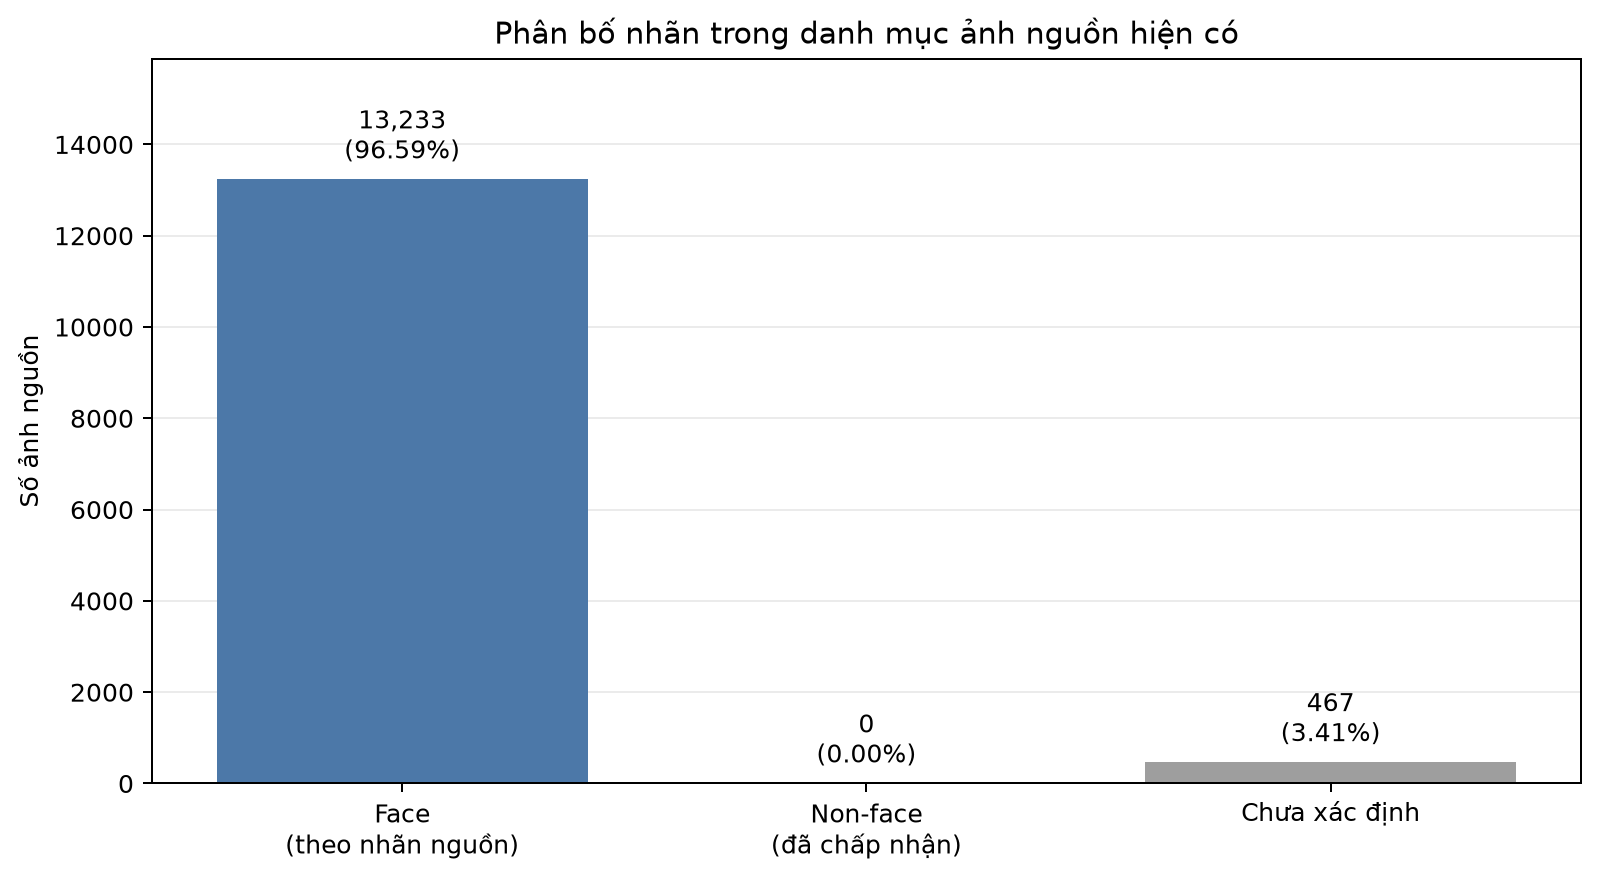
\includegraphics[width=0.85\textwidth]
        {images/eda_source_label_distribution.png}
    \caption{Phân bố nhãn trong danh mục ảnh nguồn hiện có}
    \label{fig:phanbonhan}
\end{figure}

\textit{Nhận xét:}
Có 13\,233 ảnh mang nhãn face theo nguồn LFW,
chiếm 96,59\% danh mục.
Tại thời điểm tạo biểu đồ, chưa có ảnh nền nào
được ghi nhận là mẫu non-face đã chấp nhận.
Có 467 ảnh chưa được gán nhãn mẫu, chiếm 3,41\%.

Nhóm ``Chưa xác định'' được đếm từ các nhãn còn trống,
có thể gồm ảnh chưa kiểm tra, cần xem lại hoặc bị loại
khỏi nguồn mẫu âm. Biểu đồ phản ánh cơ cấu nguồn
và tiến độ hoàn thiện nhãn, chưa thể hiện phân bố lớp
của tập huấn luyện cuối cùng.

\paragraph{Thống kê các đại lượng cường độ xám.}

Mỗi ảnh nguồn được chuyển sang ảnh xám với giá trị
pixel trong khoảng 0--255.
Đại lượng \texttt{mean\_gray} là trung bình cường độ
pixel trong một ảnh; \texttt{std\_gray} là độ lệch chuẩn
cường độ pixel trong ảnh đó.
Quá trình tính toán hoàn thành trên 13\,700 ảnh
và không ghi nhận lỗi đọc ảnh.

\begin{table}[H]
    \centering
    \caption{Tóm tắt thống kê cường độ xám theo nguồn}
    \label{tab:eda_tomtat}
    \begin{tabularx}{\textwidth}{
        >{\raggedright\arraybackslash}X r r}
        \toprule
        \textbf{Thống kê}
        & \textbf{LFW}
        & \textbf{Caltech-101} \\
        \midrule
        Trung bình của \texttt{mean\_gray}
        & 98,97 & 148,73 \\
        Độ lệch chuẩn của \texttt{mean\_gray} giữa các ảnh
        & 28,19 & 54,15 \\
        Trung bình của \texttt{std\_gray}
        & 62,70 & 64,06 \\
        Độ lệch chuẩn của \texttt{std\_gray} giữa các ảnh
        & 11,31 & 17,40 \\
        \bottomrule
    \end{tabularx}
\end{table}

\paragraph{Phân bố độ sáng và độ phân tán cường độ xám.}

Histogram được chuẩn hóa theo mật độ để so sánh
hai nguồn có số lượng ảnh khác nhau.
Tổng diện tích histogram của mỗi nguồn bằng 1;
trục tung không biểu diễn số ảnh.

\begin{figure}[H]
    \centering
    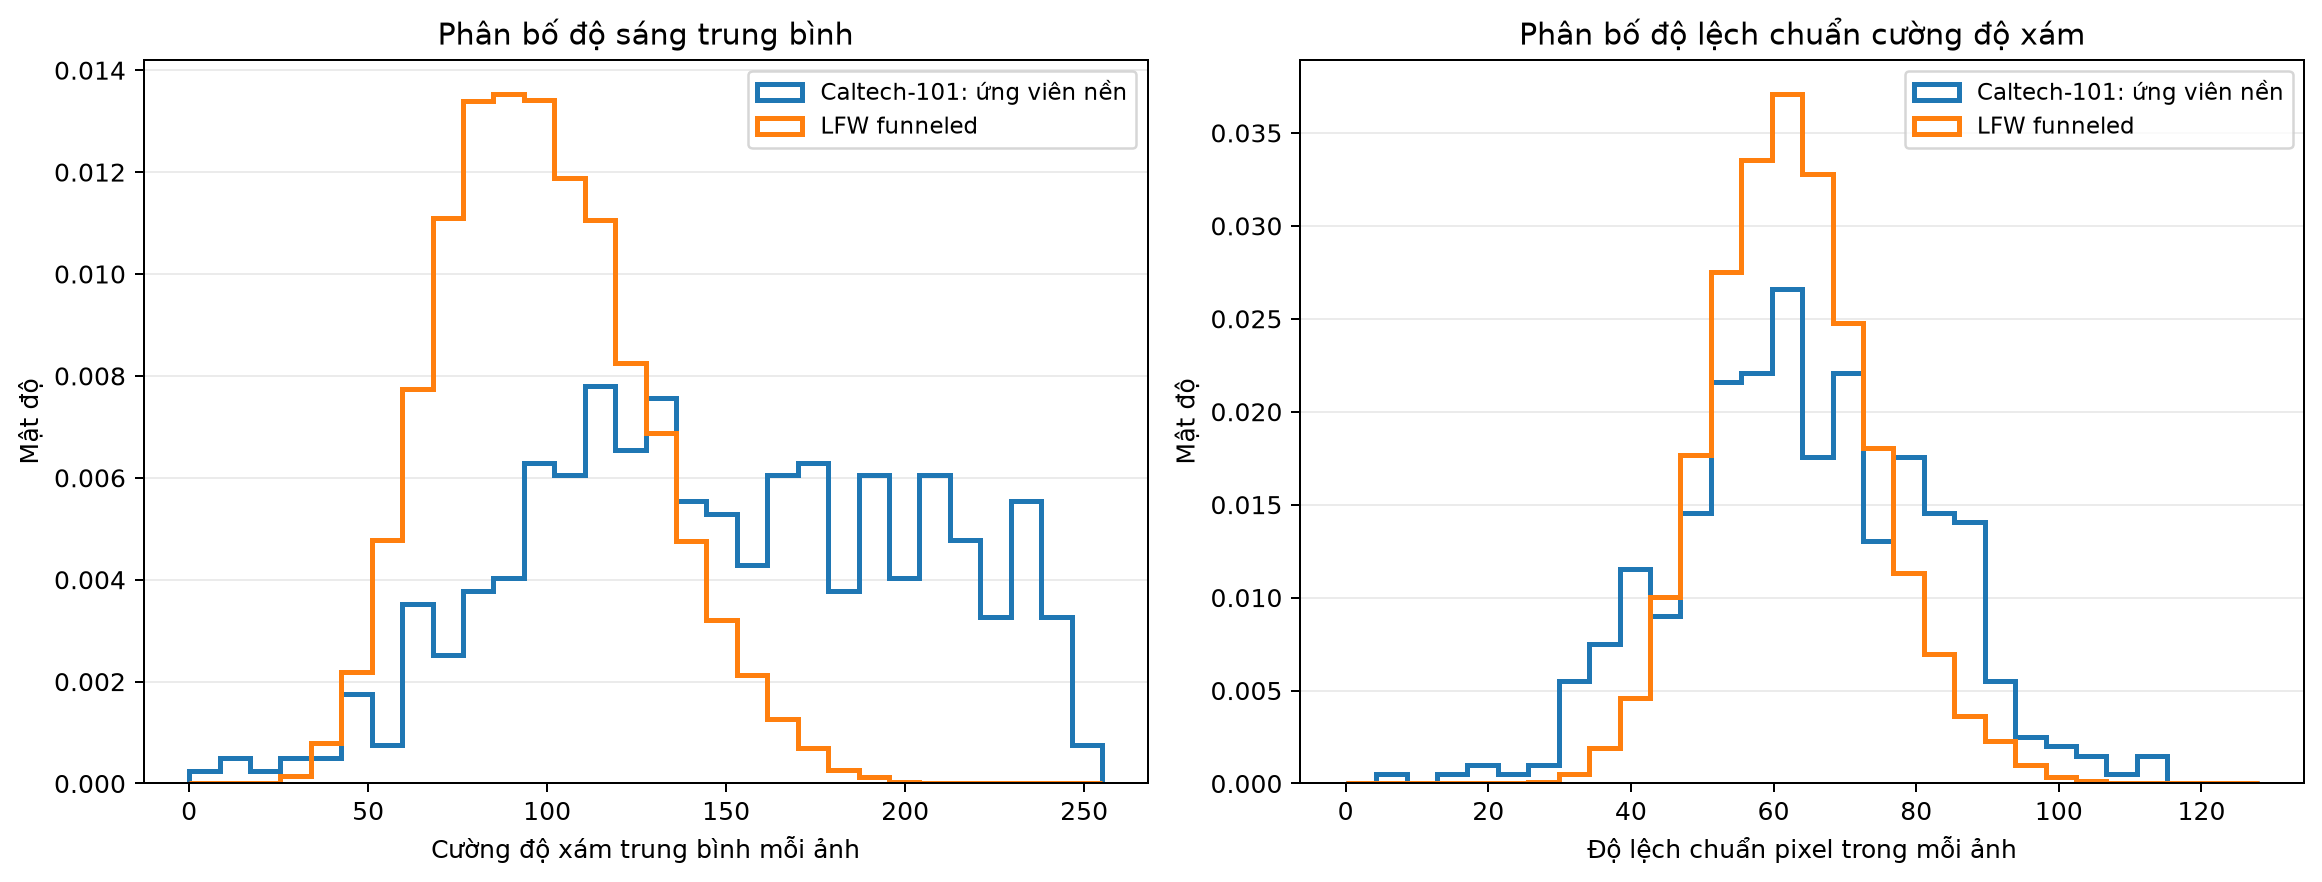
\includegraphics[width=\textwidth]
        {images/eda_brightness_contrast_by_source.png}
    \caption{Phân bố độ sáng trung bình và độ lệch chuẩn
             cường độ xám theo nguồn ảnh}
    \label{fig:eda_sang_tuongphan}
\end{figure}

\textit{Nhận xét về độ sáng:}
LFW có phân bố độ sáng trung bình tập trung chủ yếu
quanh khoảng 80--100.
Caltech-101 có phân bố trải rộng hơn và nghiêng về
phía sáng hơn; giá trị trung bình tương ứng của
hai nguồn là 98,97 và 148,73.
Tuy nhiên, hai phân bố vẫn chồng lấp đáng kể,
nên độ sáng trung bình không phân tách hoàn toàn
hai nguồn.

\textit{Nhận xét về độ lệch chuẩn cường độ xám:}
Hai phân bố chồng lấp mạnh quanh khoảng 60--70.
Trung bình của đại lượng này khá gần nhau:
62,70 đối với LFW và 64,06 đối với Caltech-101.
Caltech-101 có sự biến thiên giữa các ảnh lớn hơn,
thể hiện qua phân bố rộng hơn và độ lệch chuẩn
giữa các ảnh lớn hơn.

\textit{Giới hạn diễn giải:}
Các kết quả trên mô tả khác biệt giữa hai nguồn ảnh,
chưa thể được xem là khác biệt giữa hai lớp
face và non-face do nhãn ảnh nền chưa hoàn thiện.
Đây là các đại lượng phục vụ EDA, chưa phải
đặc trưng Haar-like và chưa chứng minh hiệu quả
phân loại của mô hình.
\subsection{Quan hệ giữa các đặc trưng}

Phân tích sử dụng hai đại lượng mô tả ảnh:
\texttt{mean\_gray} là cường độ xám trung bình và
\texttt{std\_gray} là độ lệch chuẩn cường độ pixel
trong mỗi ảnh.
Có 13\,700 dòng hợp lệ và không có dòng bị loại
do thiếu hoặc có giá trị không hữu hạn ở hai đại lượng này.

Tương quan được tính riêng theo từng nguồn nhằm
phân biệt quan hệ trong mỗi nguồn với khác biệt
giữa các nguồn.
Hệ số Pearson mô tả quan hệ tuyến tính;
hệ số Spearman mô tả xu hướng đồng biến hoặc
nghịch biến theo thứ hạng.

\begin{table}[H]
    \centering
    \caption{Tương quan giữa \texttt{mean\_gray}
             và \texttt{std\_gray} theo nguồn}
    \label{tab:tuongquan_mean_std}
    \small
    \begin{tabularx}{\textwidth}{
        >{\raggedright\arraybackslash}X r r r}
        \toprule
        \textbf{Nguồn}
        & \textbf{Số ảnh}
        & \textbf{Pearson}
        & \textbf{Spearman} \\
        \midrule
        Caltech-101: ứng viên nền
        & 467 & $-0{,}0257$ & $-0{,}0377$ \\
        LFW funneled
        & 13\,233 & $0{,}2983$ & $0{,}2820$ \\
        \bottomrule
    \end{tabularx}
\end{table}

\begin{figure}[H]
    \centering
    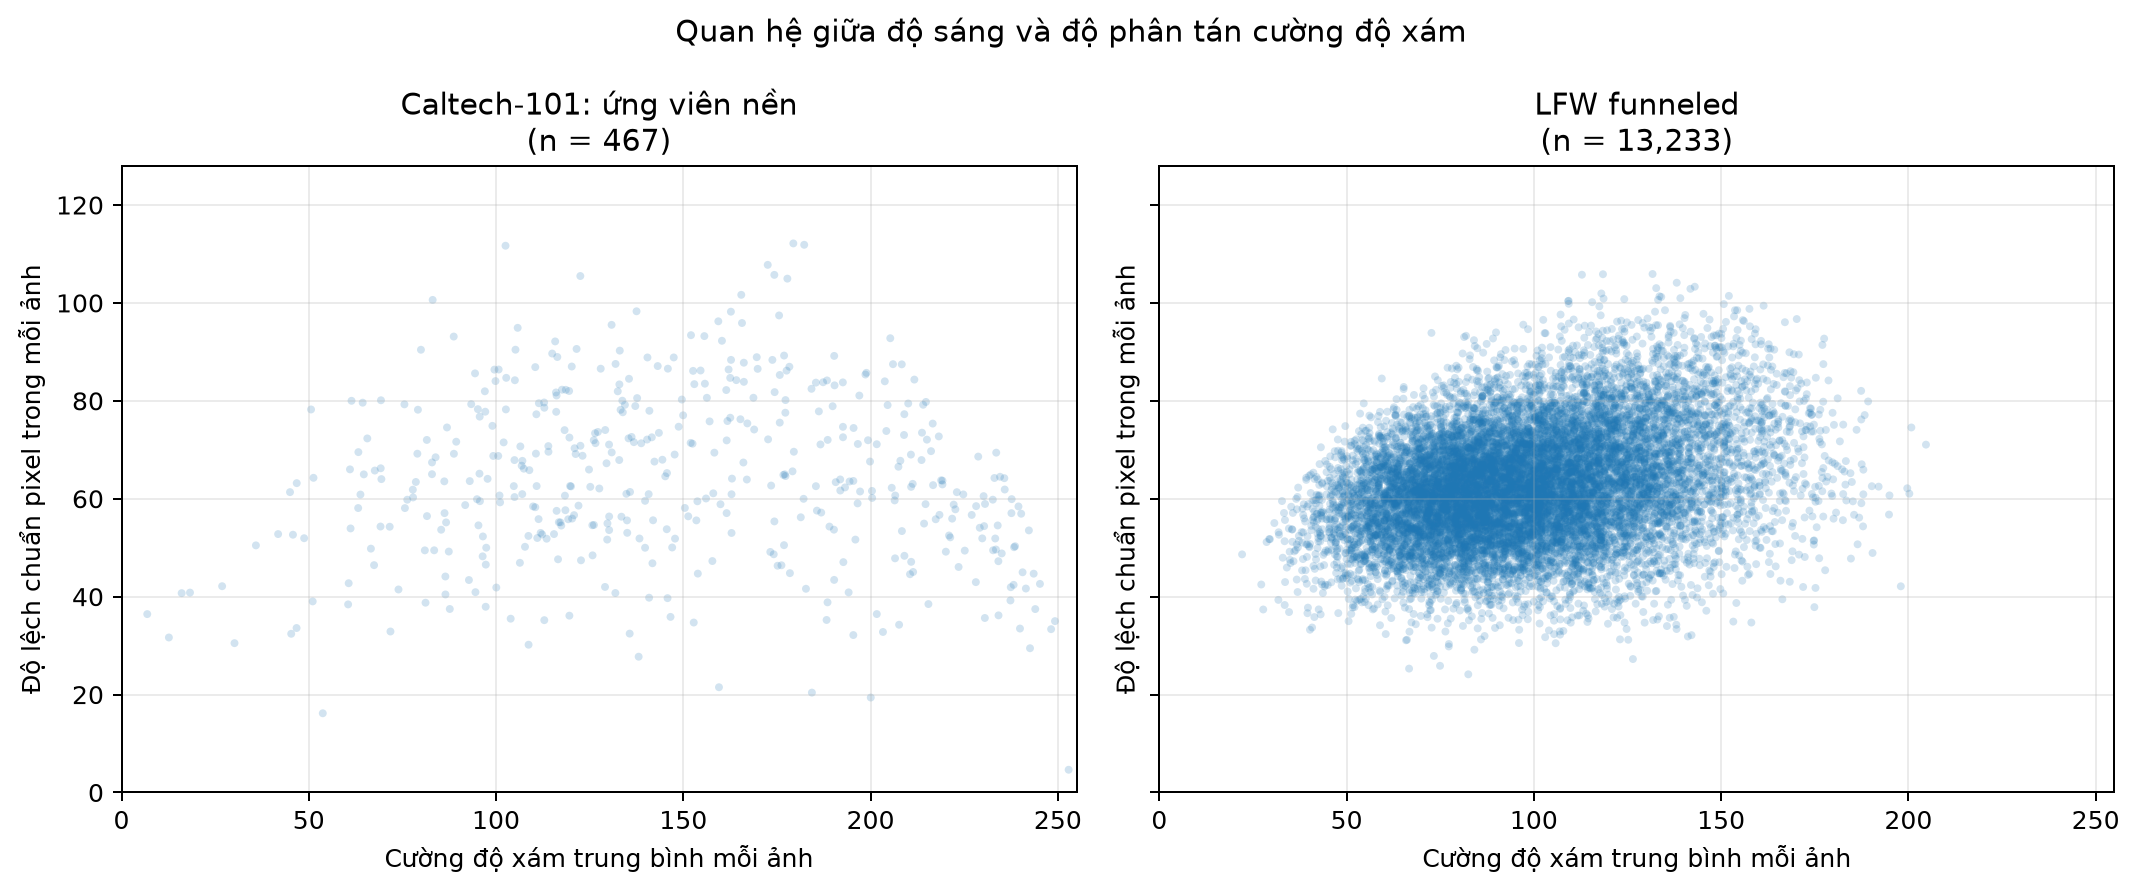
\includegraphics[width=\textwidth]
        {images/eda_mean_std_relationship_by_source.png}
    \caption{Quan hệ giữa độ sáng trung bình và độ lệch
             chuẩn cường độ xám theo từng nguồn.
             Mỗi điểm biểu diễn một ảnh; hai biểu đồ
             sử dụng cùng thang đo.}
    \label{fig:quanhe_mean_std}
\end{figure}

\paragraph{Nhận xét và ý nghĩa đối với xây dựng mô hình.}

\begin{enumerate}
    \item \textbf{LFW có xu hướng đồng biến yếu.}
    Hệ số Pearson bằng $0{,}2983$ và Spearman bằng
    $0{,}2820$ cho thấy ảnh sáng hơn có xu hướng
    có độ phân tán cường độ pixel lớn hơn.
    Tuy nhiên, các điểm vẫn phân tán đáng kể.
    Vì vậy, chưa có cơ sở xem hai đại lượng là
    thay thế cho nhau hoặc loại bỏ một đại lượng
    chỉ dựa trên tương quan này.

    \item \textbf{Caltech-101 có hệ số tương quan
    gần bằng không.}
    Pearson bằng $-0{,}0257$ và Spearman bằng
    $-0{,}0377$ cho thấy quan hệ tuyến tính và
    xu hướng đơn điệu đều rất yếu.
    Điều này không chứng minh hai đại lượng độc lập
    hoặc hoàn toàn không có quan hệ phi tuyến.
    Khi lựa chọn đặc trưng, cần kết hợp hệ số
    tương quan với biểu đồ phân tán, tránh kết luận
    chỉ từ một chỉ số.

    \item \textbf{Quan hệ giữa các đại lượng khác nhau
    theo nguồn dữ liệu.}
    LFW có đám điểm tập trung hơn, trong khi
    Caltech-101 phân tán trên phạm vi rộng hơn.
    Vì vậy, phân tích gộp có thể che khuất đặc điểm
    riêng của từng nguồn.
    Khi xây dựng và đánh giá mô hình, cần kiểm tra
    ảnh hưởng của nguồn ảnh, tránh diễn giải
    sự khác biệt theo nguồn thành khả năng
    nhận biết khuôn mặt.
\end{enumerate}

\paragraph{Phạm vi và phần cần bổ sung.}

Hai đại lượng trên mô tả độ sáng và mức phân tán
cường độ xám toàn ảnh, chưa phải đặc trưng Haar-like.
Kết quả hiện tại phục vụ phân tích quan hệ giữa
các đại lượng EDA, chưa chứng minh khả năng
phân loại của mô hình.

Do nhãn non-face của nguồn ảnh nền chưa hoàn thiện,
chưa thể kết luận về quan hệ giữa các đặc trưng
với nhãn face/non-face.
Phân tích này sẽ được bổ sung trên tập ảnh con
$24 \times 24$ có nhãn đã xác nhận để hoàn thiện
yêu cầu của Tiêu chí 5.

\subsection{Phát hiện vấn đề chất lượng dữ liệu}

Kiểm tra được thực hiện trên danh mục 13\,700 ảnh nguồn.
Sau khi duyệt nguồn nền, nhóm nguồn được chọn gồm
13\,623 ảnh: 13\,233 ảnh LFW và 390 ảnh nền Caltech-101.
Đây chưa phải tập mẫu $24 \times 24$ cuối cùng.

\begin{table}[H]
    \centering
    \caption{Kết quả kiểm tra chất lượng dữ liệu nguồn}
    \label{tab:kiemtra_chatluong_nguon}
    \small
    \begin{tabularx}{\textwidth}{
        >{\raggedright\arraybackslash}p{4.5cm}
        >{\raggedright\arraybackslash}X}
        \toprule
        \textbf{Nội dung kiểm tra}
        & \textbf{Kết quả} \\
        \midrule

        Thiếu mã ảnh hoặc đường dẫn
        & 0 trên 13\,700 ảnh nguồn. \\

        Trùng mã ảnh hoặc đường dẫn
        & 0 trên 13\,700 ảnh nguồn. \\

        Nhãn còn trống trong danh mục
        & 77 ảnh, gồm 71 ảnh bị loại khỏi nguồn nền
          và 6 ảnh chưa chắc chắn. \\

        Thiếu nhãn hoặc nhãn ngoài 0/1
        trong nhóm nguồn được chọn
        & 0 trên 13\,623 ảnh. \\

        Nhãn không nhất quán với vai trò nguồn
        & 0 ảnh LFW có nhãn khác 1;
          0 ảnh nền đã chấp nhận có nhãn khác 0. \\

        Ảnh không phù hợp làm nguồn mẫu âm
        & 71 trên 467 ảnh ứng viên được đánh dấu có mặt;
          6 ảnh chưa chắc chắn. \\

        Tệp không tồn tại hoặc lỗi giải mã
        & 0 trên 13\,700 ảnh nguồn. \\

        Đuôi tệp không phù hợp hoặc không nhận diện
        & 0 trên 13\,700 ảnh nguồn. \\

        Ảnh có chiều nhỏ hơn 24 pixel
        & 0 trên 13\,700 ảnh nguồn. \\

        Trùng nội dung chính xác
        & Không phát hiện tệp trùng SHA-256 hoặc
          ảnh trùng pixel sau chuẩn hóa hướng EXIF
          và chuyển RGB, giữ nguyên kích thước. \\

        \bottomrule
    \end{tabularx}
\end{table}

Các nhãn trống ở 77 ảnh không được tự động điền thành 0.
Những ảnh này không thuộc nhóm nguồn được chọn.
Kiểm tra trùng nội dung hiện tại chưa bao gồm
các ảnh gần giống hoặc đã thay đổi kích thước.

\paragraph{Ngoại lai của các đại lượng ảnh.}

Ngoại lai được xác định riêng trong từng nhóm nguồn
được chọn, sử dụng quy tắc:
\[
IQR = Q_3-Q_1,\qquad
x<Q_1-1{,}5IQR
\quad \text{hoặc} \quad
x>Q_3+1{,}5IQR.
\]

Không ghi nhận giá trị thiếu hoặc ngoài miền hợp lệ
ở hai đại lượng \texttt{mean\_gray} và \texttt{std\_gray}
trên 13\,623 ảnh được chọn.

\begin{table}[H]
    \centering
    \caption{Số ảnh được gắn cờ ngoại lai theo quy tắc IQR}
    \label{tab:ngoailai_iqr}
    \small
    \begin{tabularx}{\textwidth}{
        >{\raggedright\arraybackslash}X l r r}
        \toprule
        \textbf{Nhóm}
        & \textbf{Đại lượng}
        & \textbf{Số ảnh}
        & \textbf{Tỷ lệ} \\
        \midrule

        Face: LFW
        & \texttt{mean\_gray}
        & 67 & 0,51\% \\

        Face: LFW
        & \texttt{std\_gray}
        & 141 & 1,07\% \\

        Non-face: Caltech đã duyệt
        & \texttt{mean\_gray}
        & 0 & 0,00\% \\

        Non-face: Caltech đã duyệt
        & \texttt{std\_gray}
        & 1 & 0,26\% \\

        \bottomrule
    \end{tabularx}
\end{table}

Có 208 ảnh được gắn cờ ở ít nhất một đại lượng,
chiếm khoảng 1,53\% nhóm nguồn được chọn.
Một ảnh có thể được gắn cờ ở cả hai đại lượng,
nên không cộng trực tiếp các số đếm trong bảng
để tính tổng số ảnh ngoại lai.

Ngoại lai thống kê không đồng nghĩa với ảnh lỗi.
Ảnh rất tối, rất sáng hoặc có tương phản khác biệt
vẫn có thể là mẫu hợp lệ.
Riêng \texttt{mean\_gray} của nhóm Caltech đã duyệt,
cận IQR là $-14{,}46$ và $328{,}68$,
bao phủ toàn bộ miền 0--255.
Vì vậy, kết quả không có ảnh vượt cận IQR
không có nghĩa nhóm này không chứa ảnh rất tối
hoặc rất sáng.

\paragraph{Mất cân bằng số lượng ảnh nguồn.}

Trong nhóm được chọn, ảnh face chiếm 97,14\%
và ảnh non-face chiếm 2,86\%.
Tỷ lệ số ảnh face/non-face xấp xỉ 33,93:1,
cho thấy mức chênh lệch lớn ở cấp ảnh nguồn.
Phân bố này cần được cập nhật sau khi tạo
tập mẫu $24 \times 24$.

\paragraph{Nguy cơ rò rỉ dữ liệu.}

LFW không có giá trị thiếu ở trường \texttt{person\_id}.
Có 1\,680 người có nhiều hơn một ảnh,
với tổng cộng 9\,164 ảnh thuộc các nhóm này.
Nếu chia ảnh độc lập, cùng một người có thể xuất hiện
ở nhiều tập dữ liệu.

Ngoài ra, các mẫu con được tạo từ cùng một ảnh nguồn
có thể chia sẻ nội dung tương tự.
Đây là các nguy cơ cần kiểm soát khi thiết kế
cách chia tập theo người và theo ảnh nguồn.
Hiện chưa có kết quả kiểm tra giao nhau giữa
các tập để kết luận đã xảy ra rò rỉ.

\section{Chuẩn bị dữ liệu cho mô hình}
\subsection{Xử lý vấn đề chất lượng dữ liệu}

\paragraph{Lựa chọn nguồn và xử lý nhãn trống.}

Nhóm giữ toàn bộ 13\,233 ảnh LFW mang nhãn face
theo nguồn và chỉ sử dụng 390 ảnh Caltech-101
đã được chấp nhận làm nguồn non-face sau khi duyệt.

Có 71 ảnh được đánh dấu có khuôn mặt bị loại
khỏi nguồn mẫu âm; 6 ảnh chưa chắc chắn được
tạm thời không sử dụng.
Các ảnh này được lưu trong danh sách loại,
kèm lý do để có thể kiểm tra lại.

Nhãn trống của 77 ảnh không sử dụng được giữ nguyên,
không điền nhãn suy đoán.
Sau khi lọc, danh sách nguồn được chọn
không còn nhãn trống.

\begin{table}[H]
    \centering
    \caption{So sánh danh mục nguồn trước và sau bước lọc}
    \label{tab:nguon_truoc_sau_xuly}
    \small
    \begin{tabularx}{\textwidth}{
        >{\raggedright\arraybackslash}X r r}
        \toprule
        \textbf{Chỉ tiêu}
        & \textbf{Trước lọc}
        & \textbf{Sau lọc} \\
        \midrule
        Tổng số ảnh nguồn
        & 13\,700 & 13\,623 \\

        Số ảnh có nhãn trống
        & 77 & 0 \\

        Số ảnh mang nhãn face
        & 13\,233 & 13\,233 \\

        Số ảnh mang nhãn non-face
        & 390 & 390 \\

        Nguồn nền bị loại vì có mặt
        & 71 & 0 \\

        Nguồn nền chưa chắc chắn
        & 6 & 0 \\
        \bottomrule
    \end{tabularx}
\end{table}

Trong Bảng~\ref{tab:nguon_truoc_sau_xuly},
``trước lọc'' là danh mục sau khi đã duyệt ảnh,
nên đã có 390 nhãn non-face.
``Sau lọc'' chỉ gồm các nguồn được giữ.
Việc số nhãn trống giảm từ 77 xuống 0
là kết quả lựa chọn nguồn, không phải điền khuyết nhãn.

\paragraph{Xử lý các ảnh được gắn cờ ngoại lai.}

Nhóm giữ lại 208 ảnh được gắn cờ IQR,
đồng thời lưu cờ và tên đại lượng liên quan
trong metadata.
Các đại lượng của những ảnh này vẫn nằm
trong miền hợp lệ; chưa có bằng chứng cho thấy
chúng là ảnh lỗi.

Quyết định giữ ảnh nhằm bảo toàn sự đa dạng
về độ sáng và tương phản.
Không sử dụng riêng quy tắc IQR để loại bỏ
các mẫu có thể vẫn hợp lệ.
Số ảnh được giữ kèm cờ sau xử lý là 208.

\paragraph{Xử lý lỗi tệp và trùng nội dung.}

Kiểm tra không phát hiện tệp thiếu, lỗi giải mã,
đuôi tệp không phù hợp, ảnh có chiều nhỏ hơn
24 pixel hoặc nội dung trùng chính xác
theo các phương pháp đã khảo sát.
Do đó, không phát sinh thao tác sửa hoặc loại ảnh
vì các vấn đề này.

\paragraph{Chuẩn bị kiểm soát rò rỉ dữ liệu.}

Nhóm tạo trường \texttt{split\_group}:
ảnh LFW được nhóm theo \texttt{person\_id};
ảnh Caltech-101 được nhóm theo
\texttt{source\_image\_id}.
Kết quả có 6\,139 nhóm phục vụ chia tập.

Mã nhóm là thông tin chuẩn bị cho bước chia dữ liệu.
Việc giữ nhóm và kiểm tra giao nhau giữa các tập
sẽ được thực hiện trong phần chuẩn bị dữ liệu
cho mô hình.

\paragraph{Mất cân bằng và phạm vi xử lý.}

Bước xử lý nguồn giữ nguyên 13\,233 ảnh face
và 390 ảnh non-face.
Chênh lệch số lượng giữa hai nhóm chưa được
cân bằng ở bước này.
Chiến lược lấy mẫu và cân bằng sẽ được xác định
khi chuẩn bị tập mẫu cho mô hình;
nếu áp dụng lấy mẫu lại, chỉ thực hiện
trên tập huấn luyện.

Danh sách nguồn được giữ được lưu tại
\texttt{clean\_source\_manifest.csv};
danh sách nguồn không sử dụng được lưu tại
\texttt{excluded\_source\_manifest.csv}.
Các kết quả trên mô tả xử lý ảnh nguồn,
chưa phải thống kê của tập mẫu
$24 \times 24$ cuối cùng.
\section{Chuẩn bị dữ liệu cho mô hình}

\paragraph{Tạo mẫu và mã hóa nhãn.}

Bộ mẫu ban đầu gồm 1\,800 ảnh mặt từ LFW
và 1\,800 mẫu nền được cắt từ 390 ảnh Caltech-101
đã duyệt.
Các mẫu được chuyển sang ảnh xám kích thước
$24 \times 24$, kiểu \texttt{uint8},
với giá trị pixel trong khoảng 0--255.

Sau khi kiểm tra trùng pixel trên các mẫu đã
cắt và thay đổi kích thước, 11 bản sao được loại bỏ.
Bộ dữ liệu còn 3\,589 mẫu, gồm 1\,800 mẫu face
và 1\,789 mẫu non-face.
Nhãn được mã hóa trực tiếp:
\texttt{face = 1}, \texttt{non-face = 0}.

\paragraph{Chia dữ liệu theo nhóm.}

Dữ liệu được chia riêng trong từng lớp bằng
\texttt{GroupShuffleSplit}, với seed cơ sở bằng 42,
hướng tới tỷ lệ train/validation/test là 70/15/15.

Đối với LFW, nhóm được xác định theo mã người;
đối với Caltech-101, nhóm được xác định theo ảnh nền gốc.
Các mẫu thuộc cùng một nhóm được giữ trong cùng một tập.
Tỷ lệ mẫu thực tế có thể lệch nhẹ so với mục tiêu
do số mẫu trong mỗi nhóm khác nhau.

\begin{table}[H]
    \centering
    \caption{Phân bố mẫu và nhóm sau khi chia dữ liệu}
    \label{tab:chia_tap_mohinh}
    \small
    \begin{tabularx}{\textwidth}{
        >{\raggedright\arraybackslash}X r r r r r}
        \toprule
        \textbf{Tập}
        & \textbf{Non-face}
        & \textbf{Face}
        & \textbf{Tổng}
        & \textbf{Tỷ lệ}
        & \textbf{Nhóm} \\
        \midrule
        Train
        & 1\,234 & 1\,277 & 2\,511 & 69,96\% & 1\,128 \\
        Validation
        & 260 & 280 & 540 & 15,05\% & 243 \\
        Test
        & 295 & 243 & 538 & 14,99\% & 243 \\
        \midrule
        Tổng
        & 1\,789 & 1\,800 & 3\,589 & 100,00\% & 1\,614 \\
        \bottomrule
    \end{tabularx}
\end{table}

Kiểm tra từng cặp train--validation, train--test
và validation--test đều cho kết quả:
0 nhóm giao nhau, 0 hash pixel giao nhau
và 0 ảnh nền gốc giao nhau.
Các kết quả này xác nhận không có giao nhau
theo các tiêu chí đã kiểm tra;
chưa bao gồm phát hiện ảnh gần giống.

\paragraph{Biến đổi ảnh và trích xuất đặc trưng.}

Cường độ pixel được chia cho hằng số 255
để đưa về khoảng $[0,1]$.
Ảnh tích phân được sử dụng để tính nhanh
tổng cường độ trong các vùng chữ nhật.

Mỗi ảnh được biểu diễn bằng 258 đặc trưng Haar-like
cố định, gồm các mẫu hai và ba hình chữ nhật
theo chiều ngang hoặc dọc, cùng mẫu bốn hình chữ nhật.
Cạnh ô cơ sở được chọn là 4, 6 và 8 pixel,
với bước dịch 4 pixel.
Giá trị đặc trưng được chuẩn hóa theo diện tích
để biểu diễn chênh lệch cường độ giữa các vùng.

Ma trận $X$ có kích thước $3\,589 \times 258$,
kiểu \texttt{float32}, không có giá trị NaN hoặc vô hạn.
Mỗi dòng của $X$ tương ứng với một dòng metadata;
mỗi cột tương ứng với một đặc trưng trong từ điển dữ liệu.

Kích thước các ma trận sau chia tập là:
\[
X_{\mathrm{train}}: 2\,511 \times 258,\qquad
X_{\mathrm{val}}: 540 \times 258,\qquad
X_{\mathrm{test}}: 538 \times 258.
\]

Nhãn, mã người, mã nhóm và thông tin nguồn
được lưu riêng trong metadata, không đưa vào $X$.

\paragraph{Nguyên tắc sử dụng dữ liệu.}

Phép chia cho 255 và bộ đặc trưng Haar-like cố định
không cần khớp tham số từ dữ liệu.
Mọi bước lựa chọn đặc trưng theo nhãn hoặc
biến đổi cần \texttt{fit} trong giai đoạn sau
chỉ được khớp trên tập train.

Tập validation phục vụ lựa chọn cấu hình;
tập test được giữ lại cho đánh giá cuối cùng.
Ma trận đặc trưng, nhãn, metadata, từ điển đặc trưng
và các tập dữ liệu đã được lưu để sử dụng lại.
\section{Môi trường thực nghiệm}
\paragraph{Cài đặt và kiểm tra mã nguồn Python.}

Các mô hình được cài đặt trong notebook
\texttt{02\_Week6\_Training\_FaceDetection.ipynb}.
Mã nguồn được tổ chức theo các bước: nạp và kiểm tra
dữ liệu, thiết lập kiểm định chéo theo nhóm, xây dựng
Pipeline, huấn luyện, đánh giá và lưu kết quả.
Các phần mã có tiêu đề và chú thích về mục đích xử lý.

NumPy được sử dụng để xử lý ma trận đặc trưng,
pandas để quản lý metadata và bảng kết quả,
Scikit-learn để xây dựng Pipeline, mô hình phân loại
và tính các chỉ số đánh giá.

Notebook sử dụng đường dẫn tương đối và kiểm tra
các tệp đầu vào trước khi thực thi.
Dữ liệu đặc trưng đã xử lý được đóng gói cùng
mã nguồn; các phiên bản thư viện và hướng dẫn chạy
được lưu trong \texttt{requirements-week6.txt}
và \texttt{README\_WEEK6.md}.
Việc chạy lại từ đầu được sử dụng để kiểm tra
mã không phụ thuộc vào các biến còn lưu trong bộ nhớ.


\section{Kết quả huấn luyện và đánh giá}
\subsection{Kết quả kiểm định chéo trên tập huấn luyện}

Bảy mô hình được đánh giá trên cùng phân công kiểm định
chéo 5 fold theo nhóm, chỉ sử dụng 2\,511 mẫu thuộc tập
huấn luyện. Với mỗi mô hình tại mỗi fold, một Pipeline
mới được nhân bản và khớp trên phần huấn luyện của fold.
Các bước chuẩn hóa cần học tham số được đặt bên trong
Pipeline để không sử dụng phần kiểm định khi khớp tham số.

Mỗi mẫu thuộc tập train được dự đoán ngoài fold đúng
một lần cho mỗi mô hình, tạo thành 17\,577 dự đoán.
Các chỉ số được tính riêng tại từng fold, sau đó lấy
trung bình số học và độ lệch chuẩn với \texttt{ddof=0}.
ROC-AUC được tính từ điểm quyết định hoặc xác suất
của lớp face, không tính từ nhãn dự đoán nhị phân.

Hai bảng dưới đây trình bày kết quả trên phần kiểm định
của các fold. Precision, Recall và $F_1$ được tính cho
lớp dương face, tương ứng nhãn 1.

\begin{table}[H]
    \centering
    \small
    \caption{Accuracy, Precision và $F_1$ qua năm fold
    (trung bình $\pm$ độ lệch chuẩn).}
    \label{tab:cv_accuracy_precision_f1}
    \begin{tabular}{lccc}
        \toprule
        \textbf{Mô hình}
        & \textbf{Accuracy}
        & \textbf{Precision}
        & \textbf{$F_1$} \\
        \midrule
        SVM RBF
        & $0{,}9701 \pm 0{,}0091$
        & $0{,}9779 \pm 0{,}0088$
        & $0{,}9703 \pm 0{,}0093$ \\

        AdaBoost
        & $0{,}9650 \pm 0{,}0116$
        & $0{,}9613 \pm 0{,}0102$
        & $0{,}9656 \pm 0{,}0116$ \\

        Random Forest
        & $0{,}9614 \pm 0{,}0109$
        & $0{,}9723 \pm 0{,}0149$
        & $0{,}9616 \pm 0{,}0110$ \\

        Logistic Regression
        & $0{,}9439 \pm 0{,}0105$
        & $0{,}9381 \pm 0{,}0192$
        & $0{,}9453 \pm 0{,}0100$ \\

        $k$-NN
        & $0{,}9335 \pm 0{,}0100$
        & $0{,}9299 \pm 0{,}0151$
        & $0{,}9350 \pm 0{,}0099$ \\

        Decision Tree
        & $0{,}8992 \pm 0{,}0194$
        & $0{,}8907 \pm 0{,}0242$
        & $0{,}9024 \pm 0{,}0185$ \\

        DummyClassifier
        & $0{,}5086 \pm 0{,}0014$
        & $0{,}5086 \pm 0{,}0014$
        & $0{,}6742 \pm 0{,}0012$ \\
        \bottomrule
    \end{tabular}
\end{table}

\begin{table}[H]
    \centering
    \small
    \caption{DR, FPR và ROC-AUC qua năm fold
    (trung bình $\pm$ độ lệch chuẩn).}
    \label{tab:cv_dr_fpr_auc}
    \begin{tabular}{lccc}
        \toprule
        \textbf{Mô hình}
        & \textbf{Recall / DR}
        & \textbf{FPR}
        & \textbf{ROC-AUC} \\
        \midrule
        SVM RBF
        & $0{,}9632 \pm 0{,}0190$
        & $0{,}0227 \pm 0{,}0095$
        & $0{,}9934 \pm 0{,}0033$ \\

        AdaBoost
        & $0{,}9702 \pm 0{,}0193$
        & $0{,}0405 \pm 0{,}0108$
        & $0{,}9930 \pm 0{,}0037$ \\

        Random Forest
        & $0{,}9514 \pm 0{,}0196$
        & $0{,}0284 \pm 0{,}0158$
        & $0{,}9932 \pm 0{,}0035$ \\

        Logistic Regression
        & $0{,}9530 \pm 0{,}0132$
        & $0{,}0656 \pm 0{,}0218$
        & $0{,}9831 \pm 0{,}0070$ \\

        $k$-NN
        & $0{,}9405 \pm 0{,}0169$
        & $0{,}0738 \pm 0{,}0172$
        & $0{,}9711 \pm 0{,}0072$ \\

        Decision Tree
        & $0{,}9146 \pm 0{,}0177$
        & $0{,}1167 \pm 0{,}0275$
        & $0{,}9320 \pm 0{,}0246$ \\

        DummyClassifier
        & $1{,}0000 \pm 0{,}0000$
        & $1{,}0000 \pm 0{,}0000$
        & $0{,}5000 \pm 0{,}0000$ \\
        \bottomrule
    \end{tabular}
\end{table}

SVM RBF đạt $F_1$ trung bình cao nhất trong cấu hình
thực nghiệm hiện tại, tiếp theo là AdaBoost và
Random Forest. Chênh lệch $F_1$ trung bình giữa SVM RBF
và AdaBoost khoảng 0,0047. Đây là thứ tự theo kết quả
trung bình của năm fold; chưa thực hiện kiểm định
để kết luận khác biệt có ý nghĩa thống kê.

Đối với thuật toán trọng tâm AdaBoost sử dụng
Decision Stump, Recall trung bình đạt 97,02\% và
FPR đạt 4,05\%. Mô hình sử dụng đặc trưng Haar-like
và boosting để phân loại cửa sổ ảnh; kết quả này
chưa đại diện cho một hệ thống Viola--Jones hoàn chỉnh
có cascade và quét ảnh đa tỷ lệ.

So với baseline luôn dự đoán face, sáu mô hình học máy
đều giảm FPR, đồng thời duy trì Recall trung bình
trên 91\%. Điều này cho thấy lợi ích của việc học
từ đặc trưng ảnh trong phạm vi dữ liệu đã đánh giá.

Chênh lệch giữa $F_1$ huấn luyện và kiểm định lớn nhất
ở Decision Tree, khoảng 0,0606; nhỏ nhất trong sáu
mô hình học máy ở Logistic Regression, khoảng 0,0145.
Các chênh lệch này là thông tin hỗ trợ phân tích
khả năng tổng quát hóa, chưa đủ để khẳng định
nguyên nhân hoặc phân loại mức độ quá khớp.

Các kết quả trên sử dụng cấu hình khởi tạo,
chưa qua tìm kiếm siêu tham số. Tập validation giữ riêng
gồm 540 mẫu và tập test gồm 538 mẫu chưa được sử dụng
để đánh giá hiệu năng ở bước này.

\subsection{Đánh giá bằng ma trận nhầm lẫn và đường ROC}

Các hình đánh giá được xây dựng từ dự đoán ngoài fold
(Out-of-Fold, OOF) trên tập train. Mỗi mô hình có
2\,511 dự đoán, trong đó mỗi mẫu được dự đoán bởi
mô hình không được huấn luyện bằng mẫu đó hoặc
các mẫu cùng nhóm. Tập validation giữ riêng và
tập test không được sử dụng trong bước này.

\paragraph{Ma trận nhầm lẫn.}
Hình~\ref{fig:week6_oof_cm} tổng hợp số lượng dự đoán
đúng và sai của từng mô hình. Hàng biểu diễn nhãn thật,
cột biểu diễn nhãn dự đoán; lớp 0 là non-face
và lớp 1 là face.

\begin{figure}[H]
    \centering
    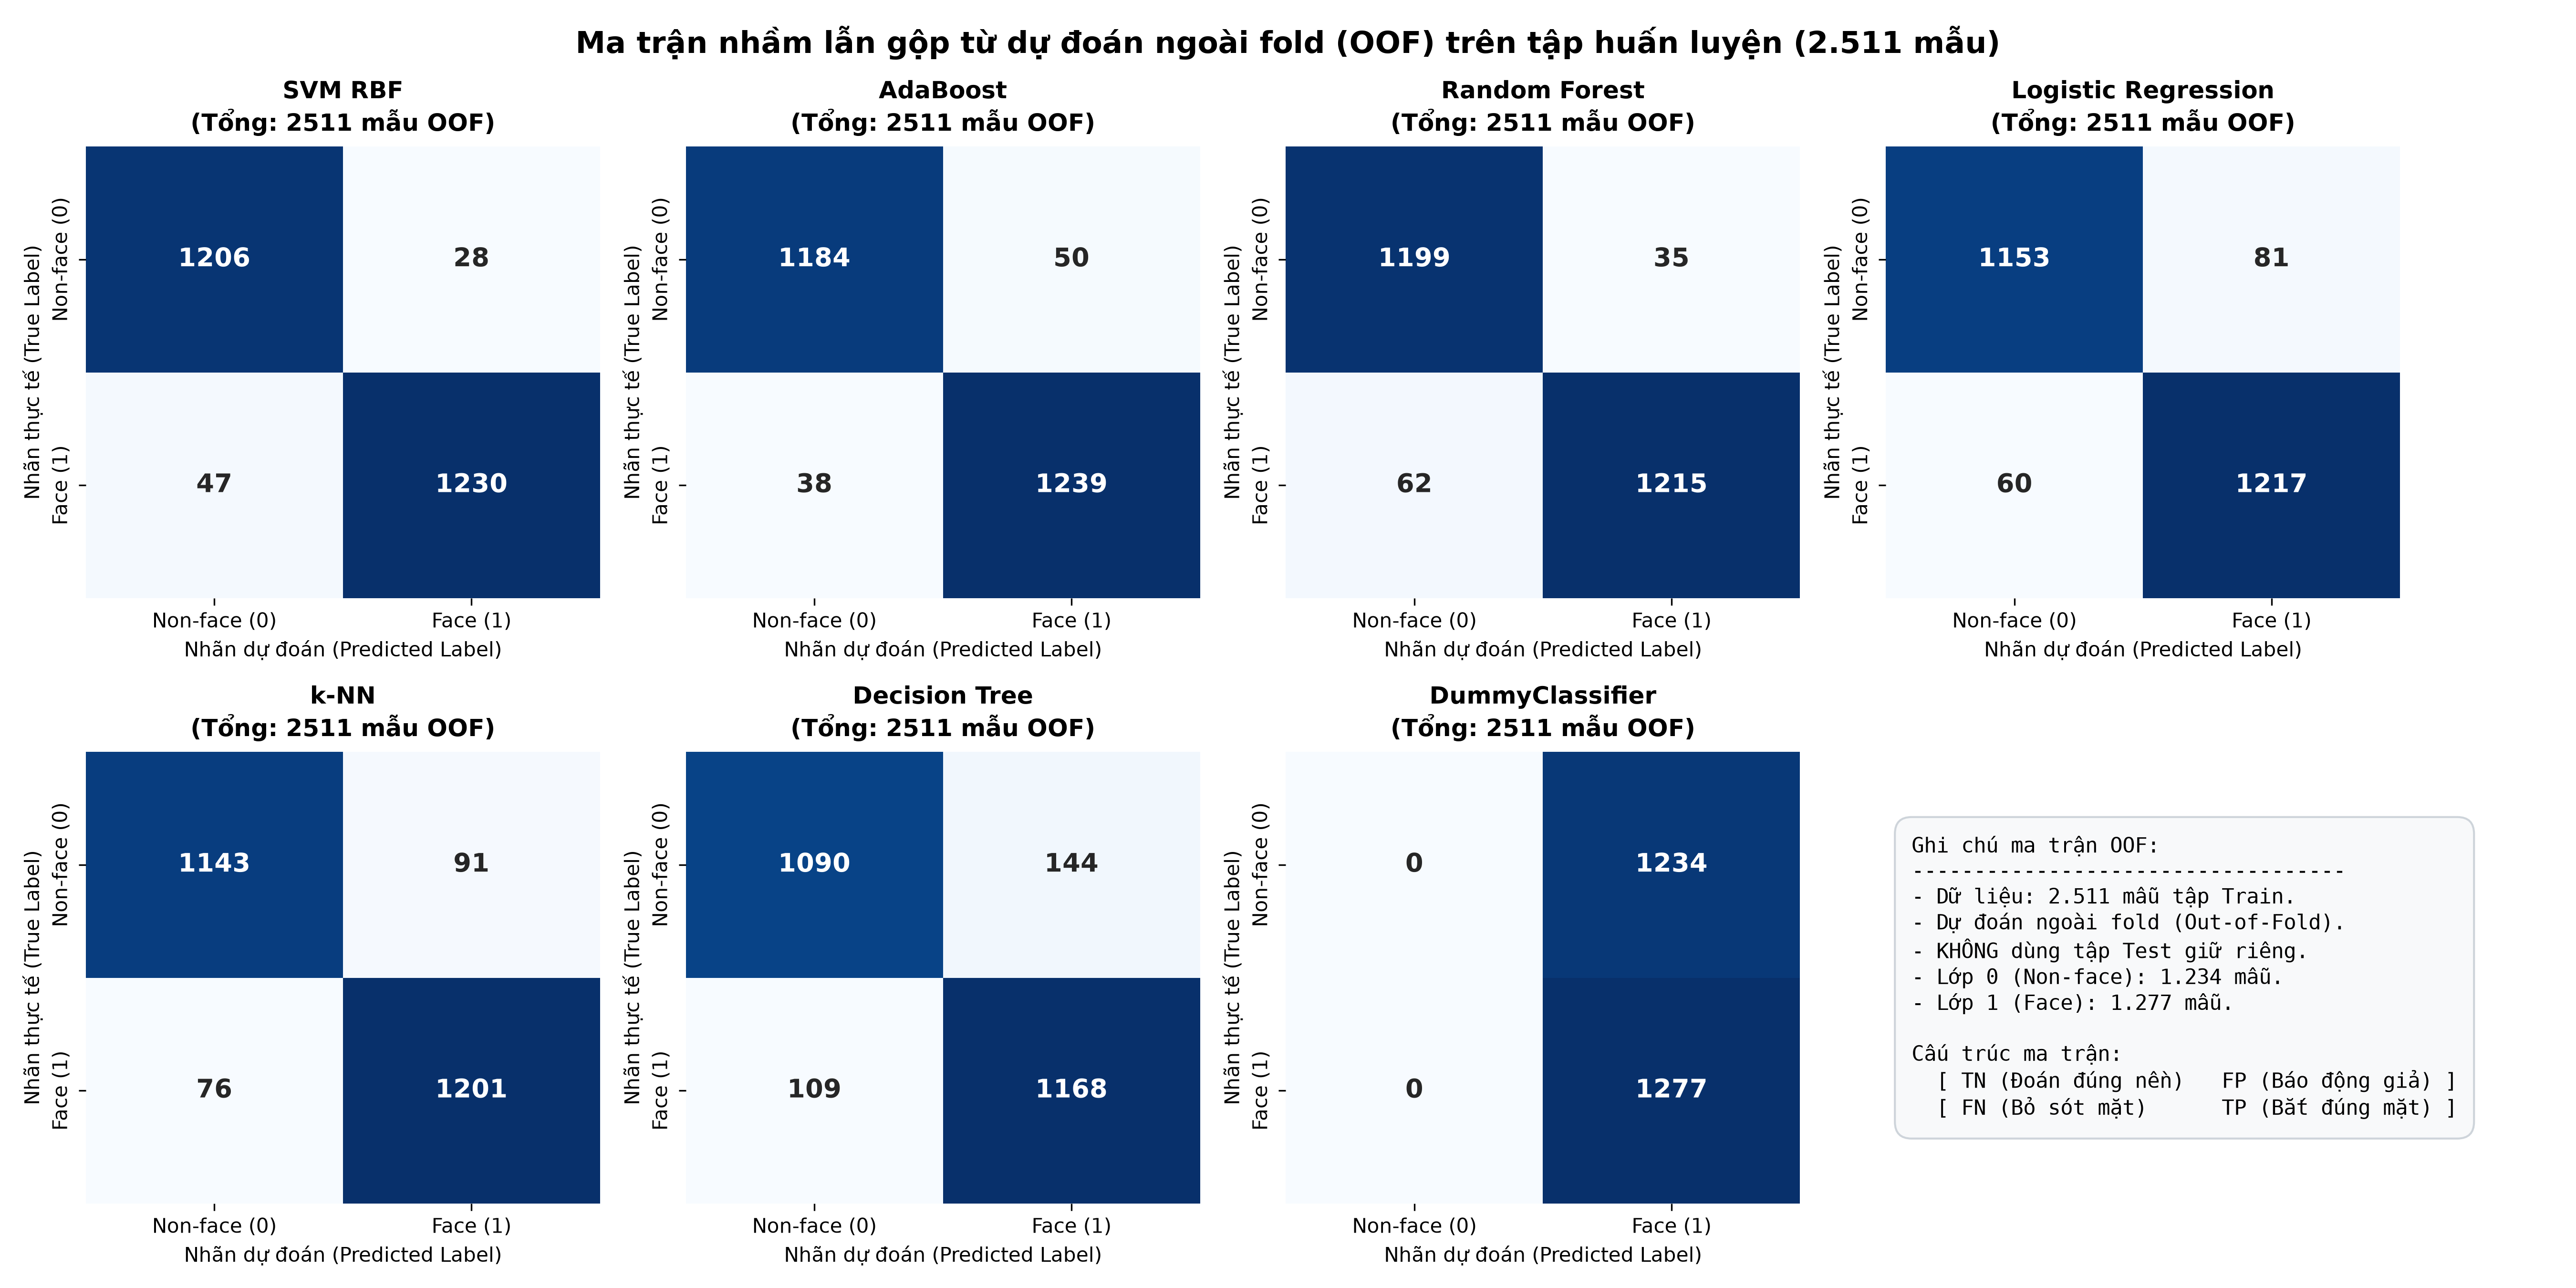
\includegraphics[
        width=\linewidth,
        height=0.78\textheight,
        keepaspectratio
    ]{images/week6_oof_confusion_matrices.png}
    \caption{Ma trận nhầm lẫn từ dự đoán OOF trên
    2\,511 mẫu train của từng mô hình.}
    \label{fig:week6_oof_cm}
\end{figure}

Trong cấu hình và cách quyết định nhãn hiện tại,
SVM RBF có ít lỗi nhận nhầm nền thành mặt nhất
trong sáu mô hình học máy, với 28 lỗi FP và 47 lỗi FN.
AdaBoost có 50 lỗi FP nhưng chỉ bỏ sót 38 mẫu mặt,
ít nhất trong sáu mô hình học máy.
Sự khác biệt này cho thấy cần xem xét đồng thời
khả năng phát hiện mặt và mức báo động giả.

DummyClassifier không bỏ sót mẫu mặt nào,
nhưng nhận nhầm toàn bộ 1\,234 mẫu nền thành mặt.
Vì vậy, Recall bằng 100\% của baseline cần được
đọc cùng FPR bằng 100\%.

Các chỉ số tính từ ma trận OOF gộp có thể khác nhẹ
trung bình chỉ số qua năm fold. Chẳng hạn,
$F_1$ gộp của SVM RBF xấp xỉ 0,9704,
trong khi trung bình $F_1$ qua các fold là 0,9703.
Đây là hai cách tổng hợp khác nhau.

\paragraph{Đường ROC trung bình.}
ROC được tính riêng tại từng fold từ điểm dự đoán.
Sau đó, TPR được nội suy trên lưới 500 giá trị FPR
chung để tính đường trung bình.
AUC trong chú giải là trung bình và độ lệch chuẩn
của các AUC từng fold.

\begin{figure}[H]
    \centering
    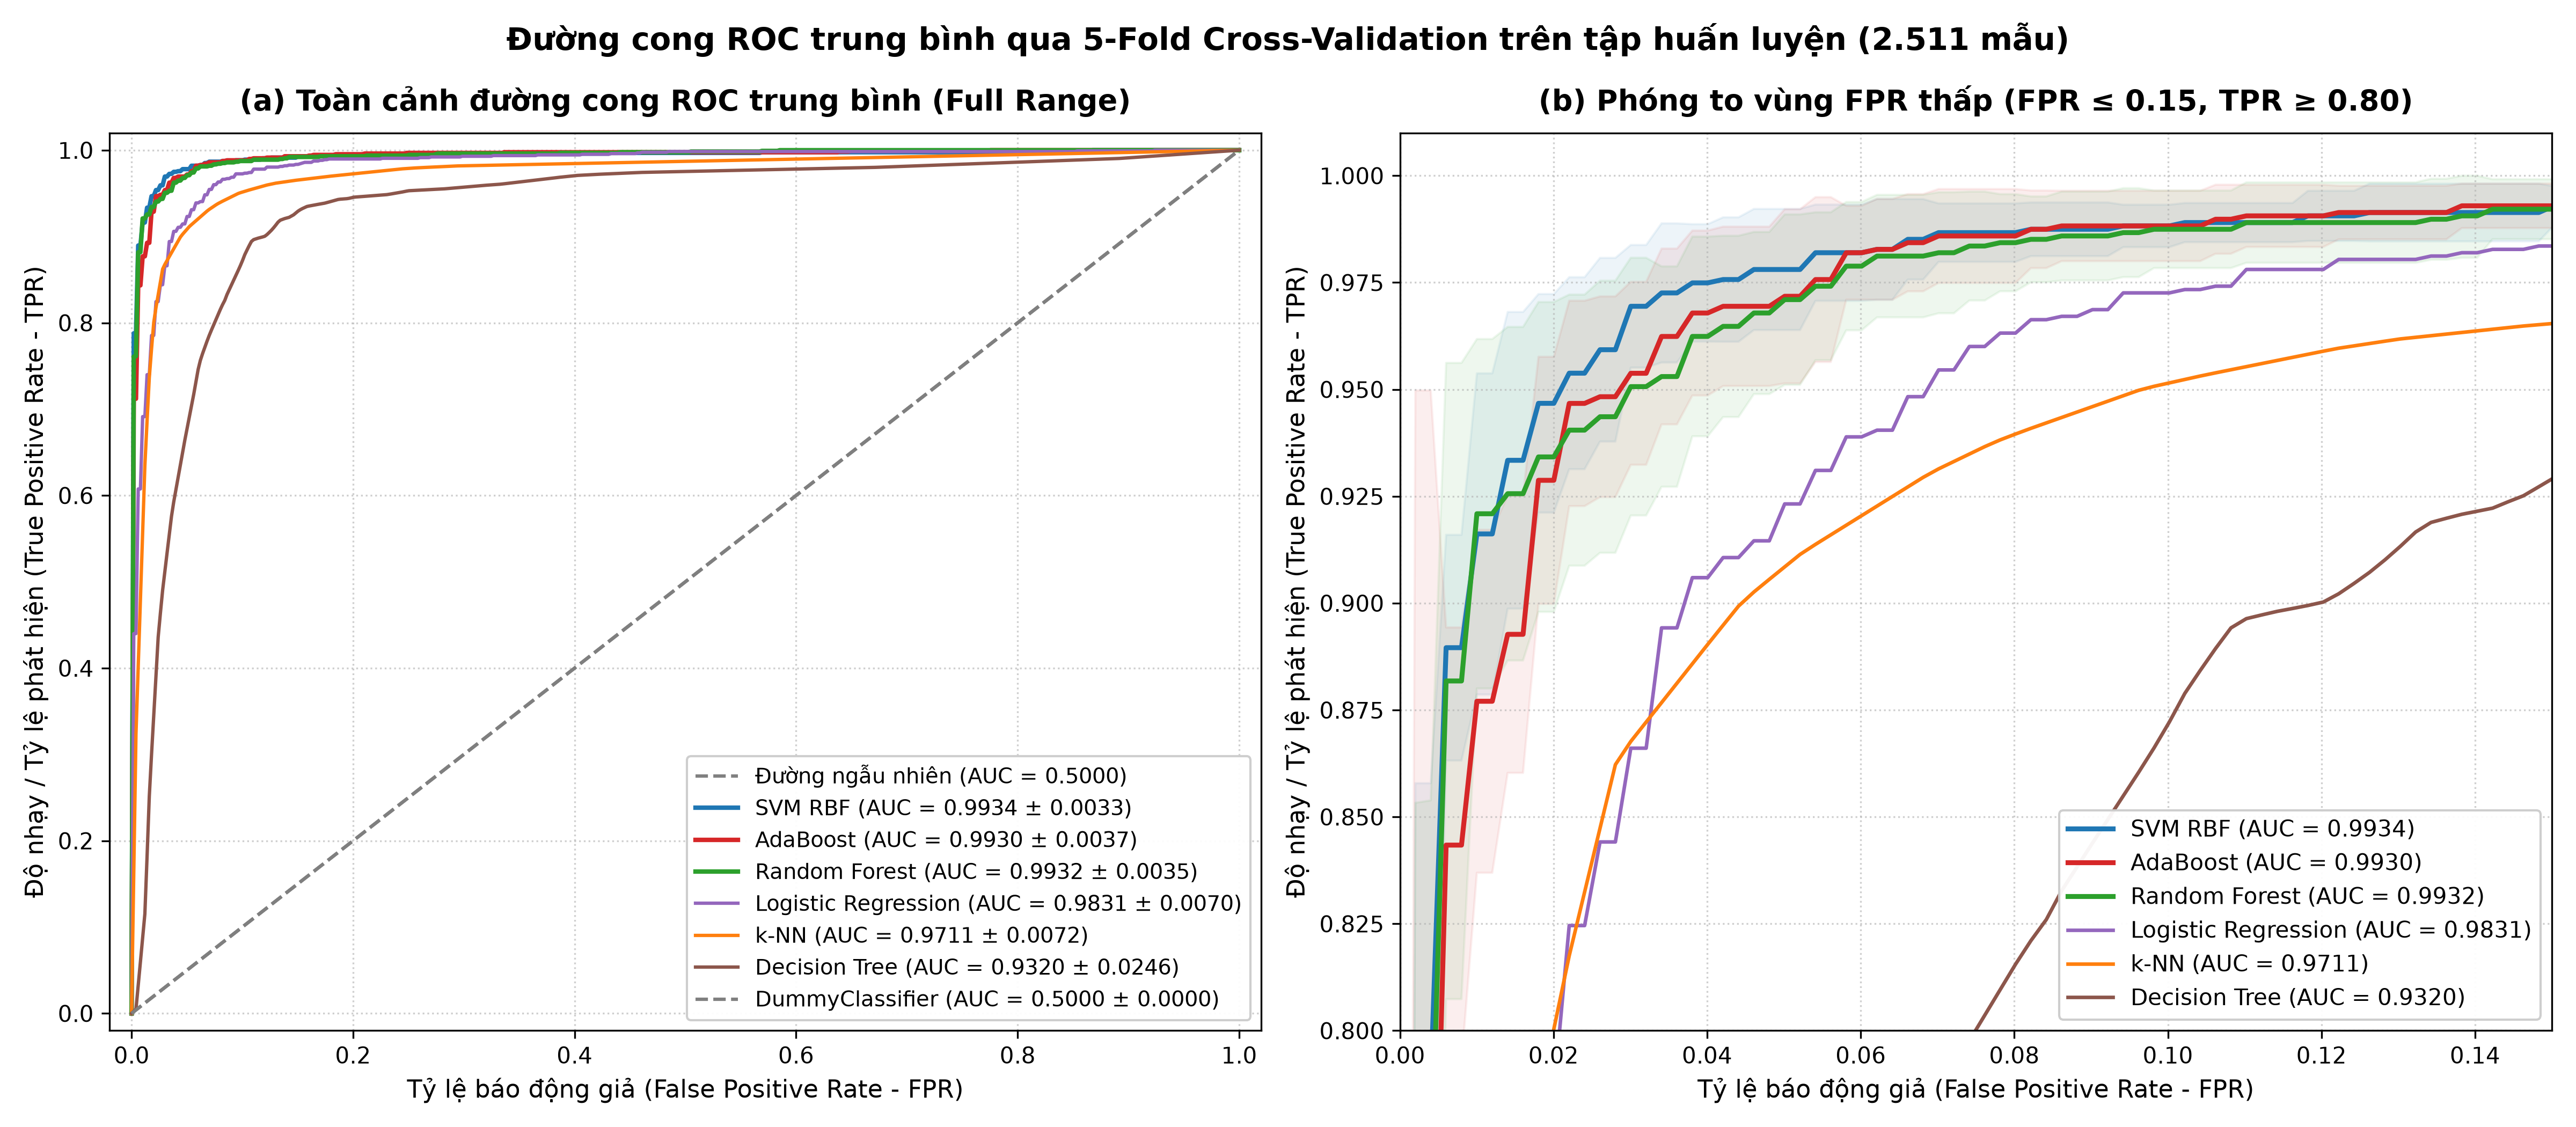
\includegraphics[
        width=\linewidth,
        height=0.78\textheight,
        keepaspectratio
    ]{images/week6_cv_mean_roc.png}
    \caption{ROC trung bình qua năm fold:
    toàn dải và vùng FPR thấp.
    Dải tô biểu diễn TPR trung bình cộng/trừ
    một độ lệch chuẩn qua các fold.}
    \label{fig:week6_cv_roc}
\end{figure}

SVM RBF, Random Forest và AdaBoost có ROC-AUC
trung bình xấp xỉ 0,993, cao hơn baseline có AUC
bằng 0,5. Khung phóng to giúp quan sát sự khác biệt
giữa các mô hình trong vùng báo động giả thấp.

Dải độ lệch chuẩn mô tả mức biến thiên giữa các fold,
không phải khoảng tin cậy và không xác nhận khác biệt
có ý nghĩa thống kê giữa các thuật toán.
Các kết quả này đánh giá phân loại cửa sổ ảnh
$24 \times 24$, chưa phản ánh hiệu quả định vị
khuôn mặt trên ảnh đầy đủ.
\section{Phân tích kết quả dự đoán}
\subsection{Đối chiếu kết quả huấn luyện và kiểm định}

Bảng~\ref{tab:train_cv_f1} đối chiếu $F_1$ trên phần
huấn luyện và phần kiểm định của năm fold.
Các giá trị được trình bày dưới dạng trung bình
$\pm$ độ lệch chuẩn, với \texttt{ddof=0}.

\begin{table}[htbp]
    \centering
    \small
    \caption{Đối chiếu $F_1$ huấn luyện và kiểm định CV.}
    \label{tab:train_cv_f1}
    \begin{tabular}{lccc}
        \toprule
        \textbf{Mô hình}
        & \textbf{$F_1$ huấn luyện}
        & \textbf{$F_1$ kiểm định}
        & \textbf{$\Delta F_1$} \\
        \midrule
        SVM RBF
        & $0{,}9884 \pm 0{,}0011$
        & $0{,}9703 \pm 0{,}0093$
        & $0{,}0181$ \\

        AdaBoost
        & $0{,}9936 \pm 0{,}0015$
        & $0{,}9656 \pm 0{,}0116$
        & $0{,}0280$ \\

        Random Forest
        & $0{,}9997 \pm 0{,}0002$
        & $0{,}9616 \pm 0{,}0110$
        & $0{,}0381$ \\

        Logistic Regression
        & $0{,}9598 \pm 0{,}0023$
        & $0{,}9453 \pm 0{,}0100$
        & $0{,}0145$ \\

        $k$-NN
        & $0{,}9561 \pm 0{,}0008$
        & $0{,}9350 \pm 0{,}0099$
        & $0{,}0211$ \\

        Decision Tree
        & $0{,}9629 \pm 0{,}0039$
        & $0{,}9024 \pm 0{,}0185$
        & $0{,}0606$ \\

        DummyClassifier
        & $0{,}6742 \pm 0{,}0003$
        & $0{,}6742 \pm 0{,}0012$
        & $\approx 0$ \\
        \bottomrule
    \end{tabular}
\end{table}

Trong đó,
$\Delta F_1=\overline{F}_{1,\mathrm{train}}
-\overline{F}_{1,\mathrm{CV}}$.
Decision Tree có mức giảm điểm lớn nhất, khoảng 0,0606,
dù đã giới hạn độ sâu ở 5.
Đây là dấu hiệu cần xem xét về khả năng tổng quát hóa
của cấu hình đang sử dụng.

Logistic Regression có mức chênh lệch nhỏ nhất trong
sáu mô hình học máy, nhưng $F_1$ kiểm định thấp hơn
SVM RBF và AdaBoost. Vì vậy, cần đọc đồng thời điểm
kiểm định và chênh lệch huấn luyện--kiểm định.
Chênh lệch gần bằng không của DummyClassifier cũng
không chứng minh mô hình tốt, bởi baseline có
FPR bằng 100\%.

Các kết quả này chưa đủ để xác định nguyên nhân
của chênh lệch hoặc gán mức độ quá khớp bằng
những ngưỡng tùy chọn.

\subsection{Phân tích các nhóm phát sinh lỗi}

Sáu mô hình học máy tạo ra tổng cộng 821 bản ghi
dự đoán sai, liên quan đến 442 ảnh khác nhau.
Một ảnh có thể xuất hiện trong bảng lỗi của nhiều
mô hình nên số bản ghi không đồng nghĩa với
số ảnh phân biệt.

AdaBoost có 88 lỗi thuộc 84 nhóm; SVM RBF có 75 lỗi
thuộc 69 nhóm. Với hai mô hình này, số lỗi tối đa
trong một nhóm là 2, cho thấy lỗi không tập trung
vào một nhóm đơn lẻ trong tập dữ liệu đang xét.

\begin{table}[htbp]
    \centering
    \small
    \caption{Một số nhóm phát sinh lỗi của
    AdaBoost và SVM RBF.}
    \label{tab:error_groups}
    \begin{tabular}{llcrrr}
        \toprule
        \textbf{Mô hình}
        & \textbf{Nhóm}
        & \textbf{Nhãn}
        & \textbf{Mẫu}
        & \textbf{Lỗi}
        & \textbf{Tỷ lệ} \\
        \midrule
        AdaBoost & \texttt{image\_0349.jpg}
        & 0 & 5 & 2 & $40{,}0\%$ \\
        AdaBoost & \texttt{image\_0403.jpg}
        & 0 & 4 & 2 & $50{,}0\%$ \\
        AdaBoost & \texttt{lfw\_person:2058}
        & 1 & 3 & 2 & $66{,}7\%$ \\
        AdaBoost & \texttt{lfw\_person:2750}
        & 1 & 2 & 2 & $100{,}0\%$ \\
        \midrule
        SVM RBF & \texttt{image\_0401.jpg}
        & 0 & 5 & 2 & $40{,}0\%$ \\
        SVM RBF & \texttt{image\_0406.jpg}
        & 0 & 5 & 2 & $40{,}0\%$ \\
        SVM RBF & \texttt{lfw\_person:2058}
        & 1 & 3 & 2 & $66{,}7\%$ \\
        SVM RBF & \texttt{lfw\_person:2750}
        & 1 & 2 & 2 & $100{,}0\%$ \\
        \bottomrule
    \end{tabular}
\end{table}

Các nhóm \texttt{image\_*.jpg} trong bảng là ảnh nền
Caltech; các nhóm \texttt{lfw\_person:*} được xác định
theo người trong LFW. Tỷ lệ lỗi được tính bằng
số mẫu sai chia tổng số mẫu OOF của nhóm.

Nhóm \texttt{lfw\_person:2750} có tỷ lệ lỗi 100\%
nhưng chỉ gồm hai mẫu. Kết quả này mô tả hai ảnh
đang xét, chưa đủ để suy rộng sang các ảnh khác
của cùng người. Ngược lại, nhóm
\texttt{lfw\_person:1871} gồm 70 mẫu có một lỗi
ở AdaBoost và không có lỗi ở SVM RBF; đây cũng
chỉ là kết quả quan sát trên nhóm đã đánh giá.

\subsection{Quan sát các ảnh dự đoán sai}

Hai hình dưới đây minh họa tối đa tám FP và tám FN
cho mỗi mô hình. Các mẫu được chọn tái lập với
\texttt{random\_state=42}, ưu tiên những nhóm khác nhau
trong từng mô hình. Mã chỉ số trên hình tương ứng
với \texttt{global\_row\_index} trong bảng minh chứng.

\begin{figure}[htbp]
    \centering
    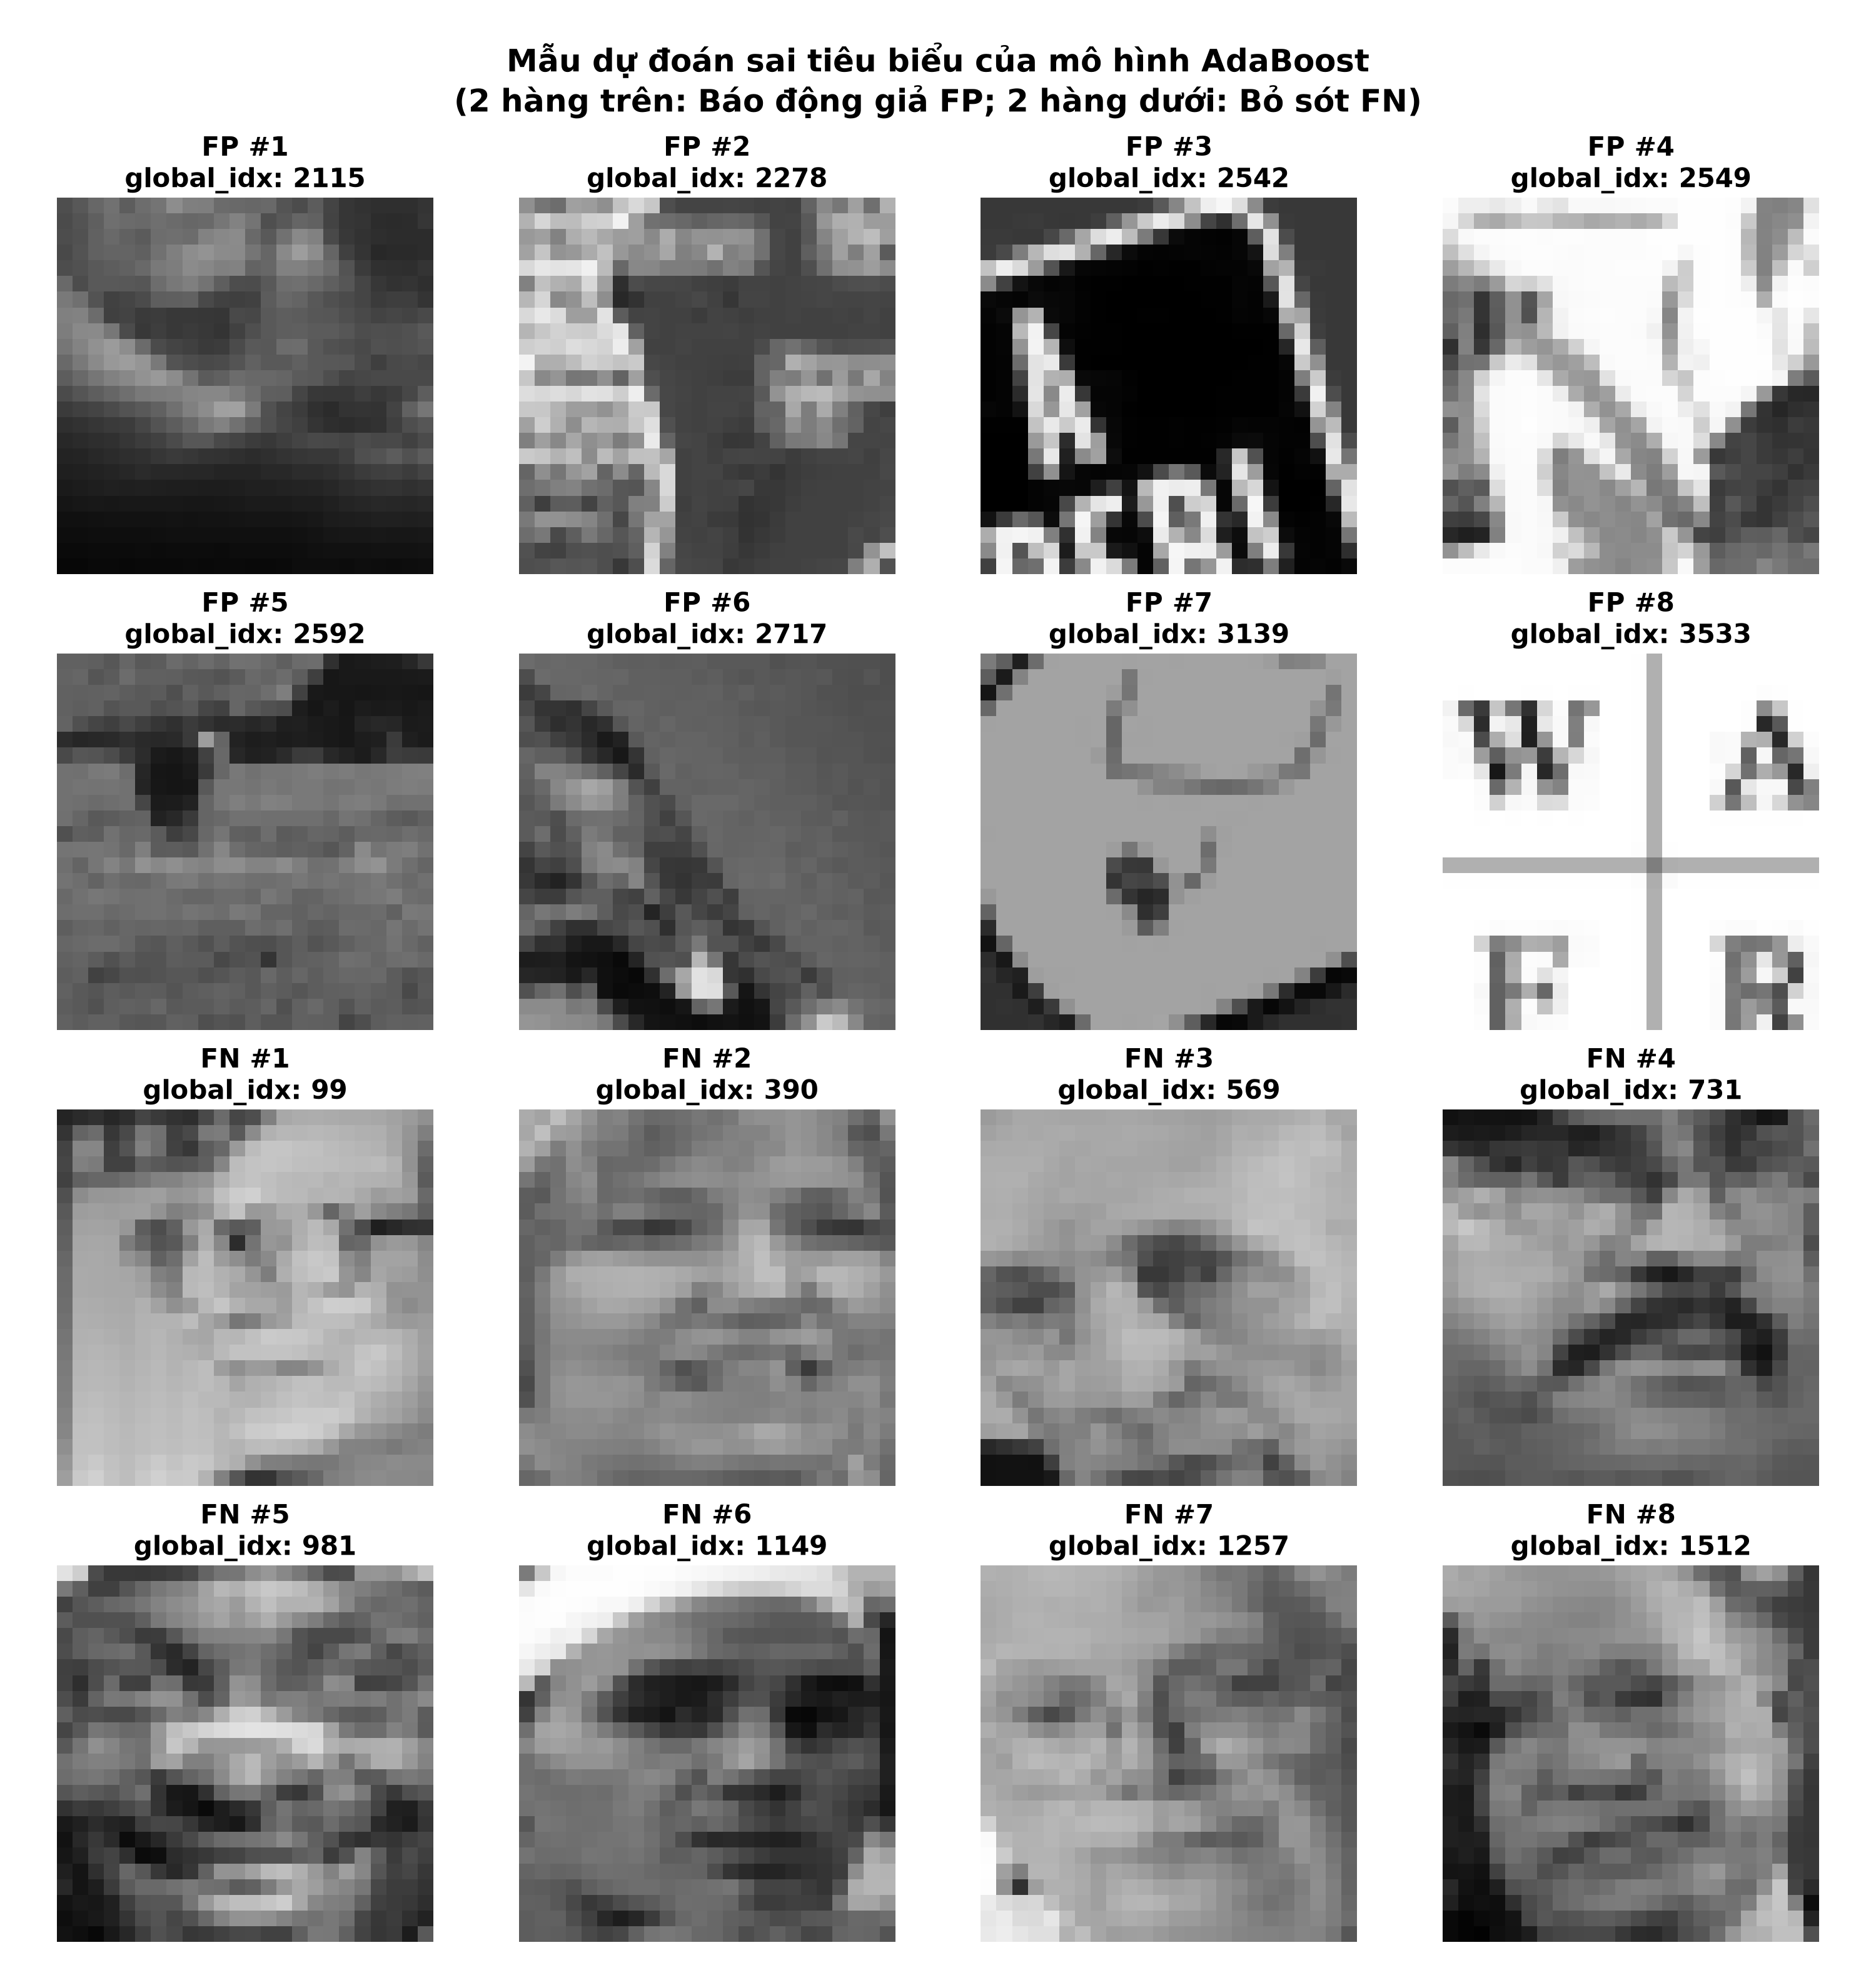
\includegraphics[
        width=\linewidth,
        height=0.76\textheight,
        keepaspectratio
    ]{images/week6_errors_adaboost.png}
    \caption{Mẫu lỗi của AdaBoost:
    hai hàng trên là FP, hai hàng dưới là FN.}
    \label{fig:errors_adaboost}
\end{figure}

\begin{figure}[htbp]
    \centering
    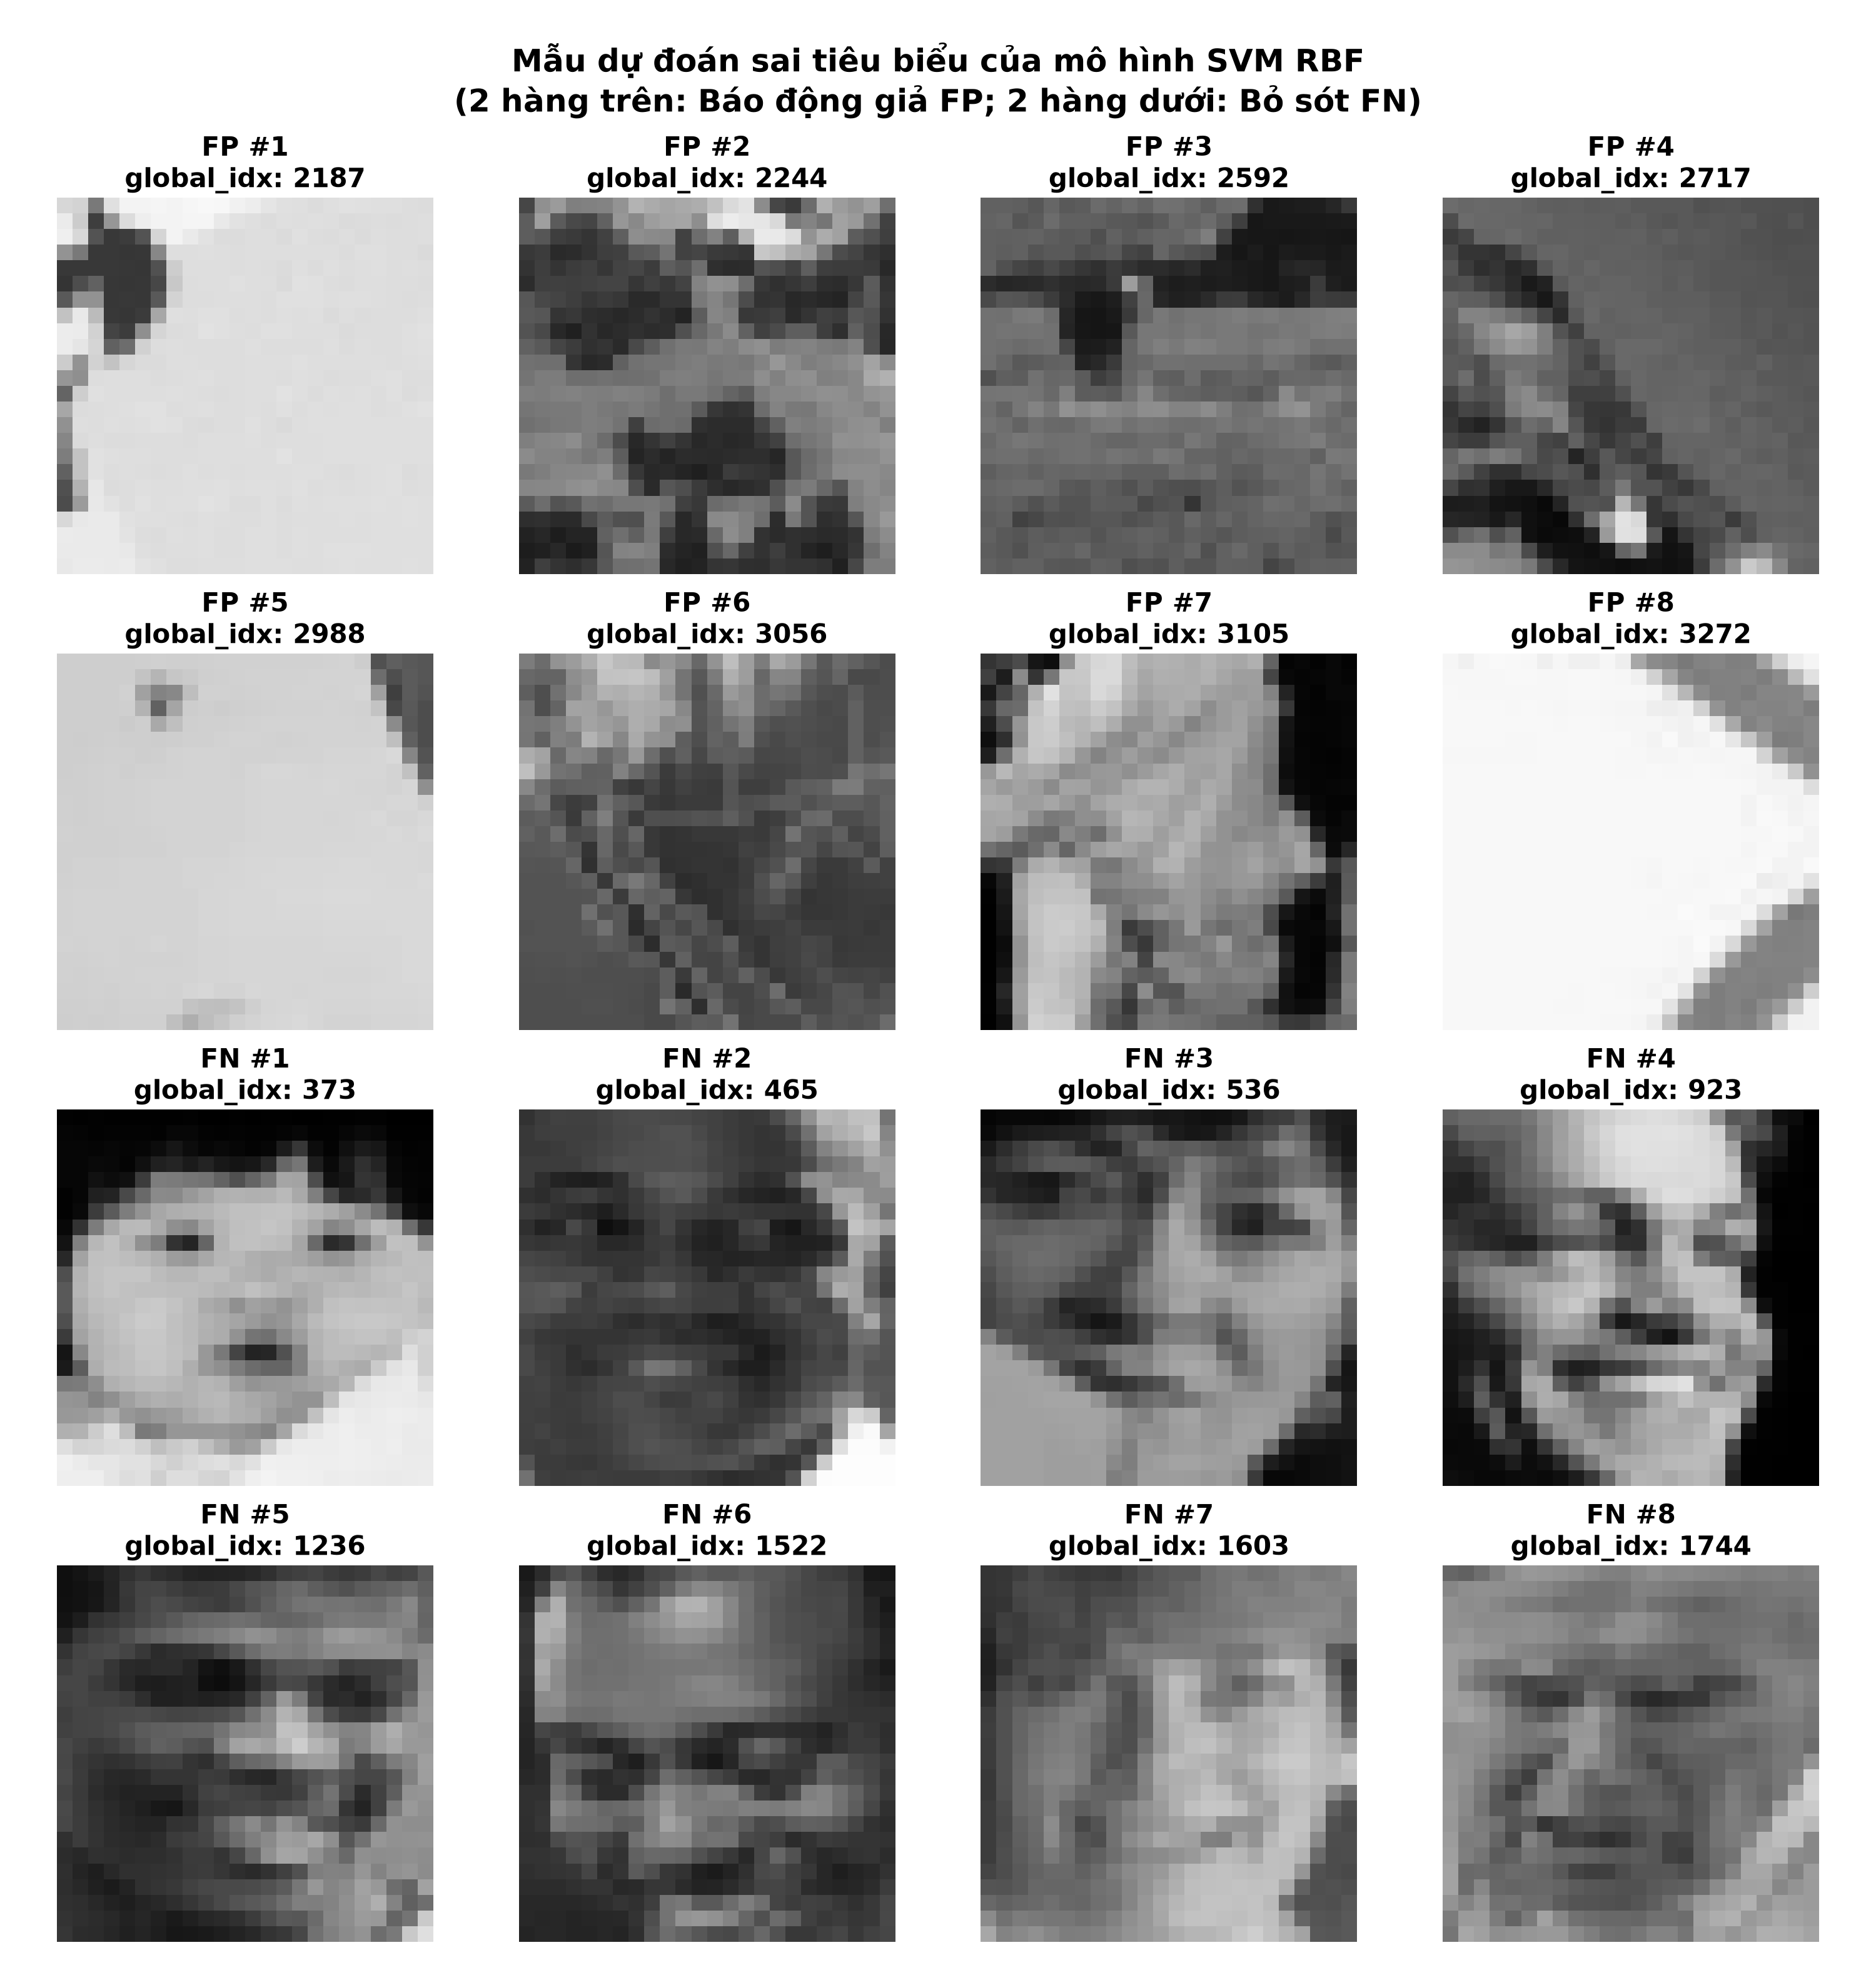
\includegraphics[
        width=\linewidth,
        height=0.76\textheight,
        keepaspectratio
    ]{images/week6_errors_svm_rbf.png}
    \caption{Mẫu lỗi của SVM RBF:
    hai hàng trên là FP, hai hàng dưới là FN.}
    \label{fig:errors_svm_rbf}
\end{figure}

Trong các mẫu FP được chọn, có những vùng nền chứa
đường viền hoặc các dải sáng--tối rõ rệt.
Mẫu 3533 có nền sáng và các nét đậm, với cường độ
xám trung bình khoảng 224,89.
Hai mẫu 2592 và 2717 bị cả AdaBoost và SVM RBF
nhận nhầm, có độ lệch chuẩn cường độ xám lần lượt
khoảng 29,90 và 30,21.

Các mẫu FN minh họa có sự khác nhau về độ sáng,
hướng khuôn mặt và mức tương phản.
Chẳng hạn, mẫu 465 có cường độ xám trung bình
khoảng 78,71; một số mẫu có vùng quanh mắt tối
hoặc chênh lệch sáng--tối rõ trong cửa sổ ảnh.

Những đặc điểm này gợi ý các trường hợp cần khảo sát
thêm, chưa chứng minh nguyên nhân khiến mô hình
dự đoán sai. Đặc biệt, độ lệch chuẩn cường độ xám
của cả ô ảnh không đủ để xác định bóng đổ trên mặt
hay đặc trưng nào đã chi phối dự đoán.

Toàn bộ phân tích sử dụng dự đoán OOF trên tập train.
Các mẫu lỗi được giữ nguyên nhãn và không bị loại bỏ.
Tập validation giữ riêng và tập test chưa được
sử dụng trong bước phân tích này.


\section{Tối ưu hóa và cải tiến mô hình}
\subsection{Phân tích hạn chế của mô hình ban đầu}
\label{subsec:week8_baseline_limitations}

Phân tích sử dụng kết quả kiểm định chéo theo nhóm trên 2.511 ảnh con
kích thước $24 \times 24$ của tập huấn luyện. Bảng~\ref{tab:train_cv_f1}
và Hình~\ref{fig:week8_f1_train_cv} đối chiếu $F_1$ của lớp khuôn mặt
giữa phần huấn luyện và phần kiểm định của năm fold. Kết quả được trình
bày bằng trung bình và độ lệch chuẩn với \texttt{ddof=0}.

\begin{figure}[htbp]
    \centering
    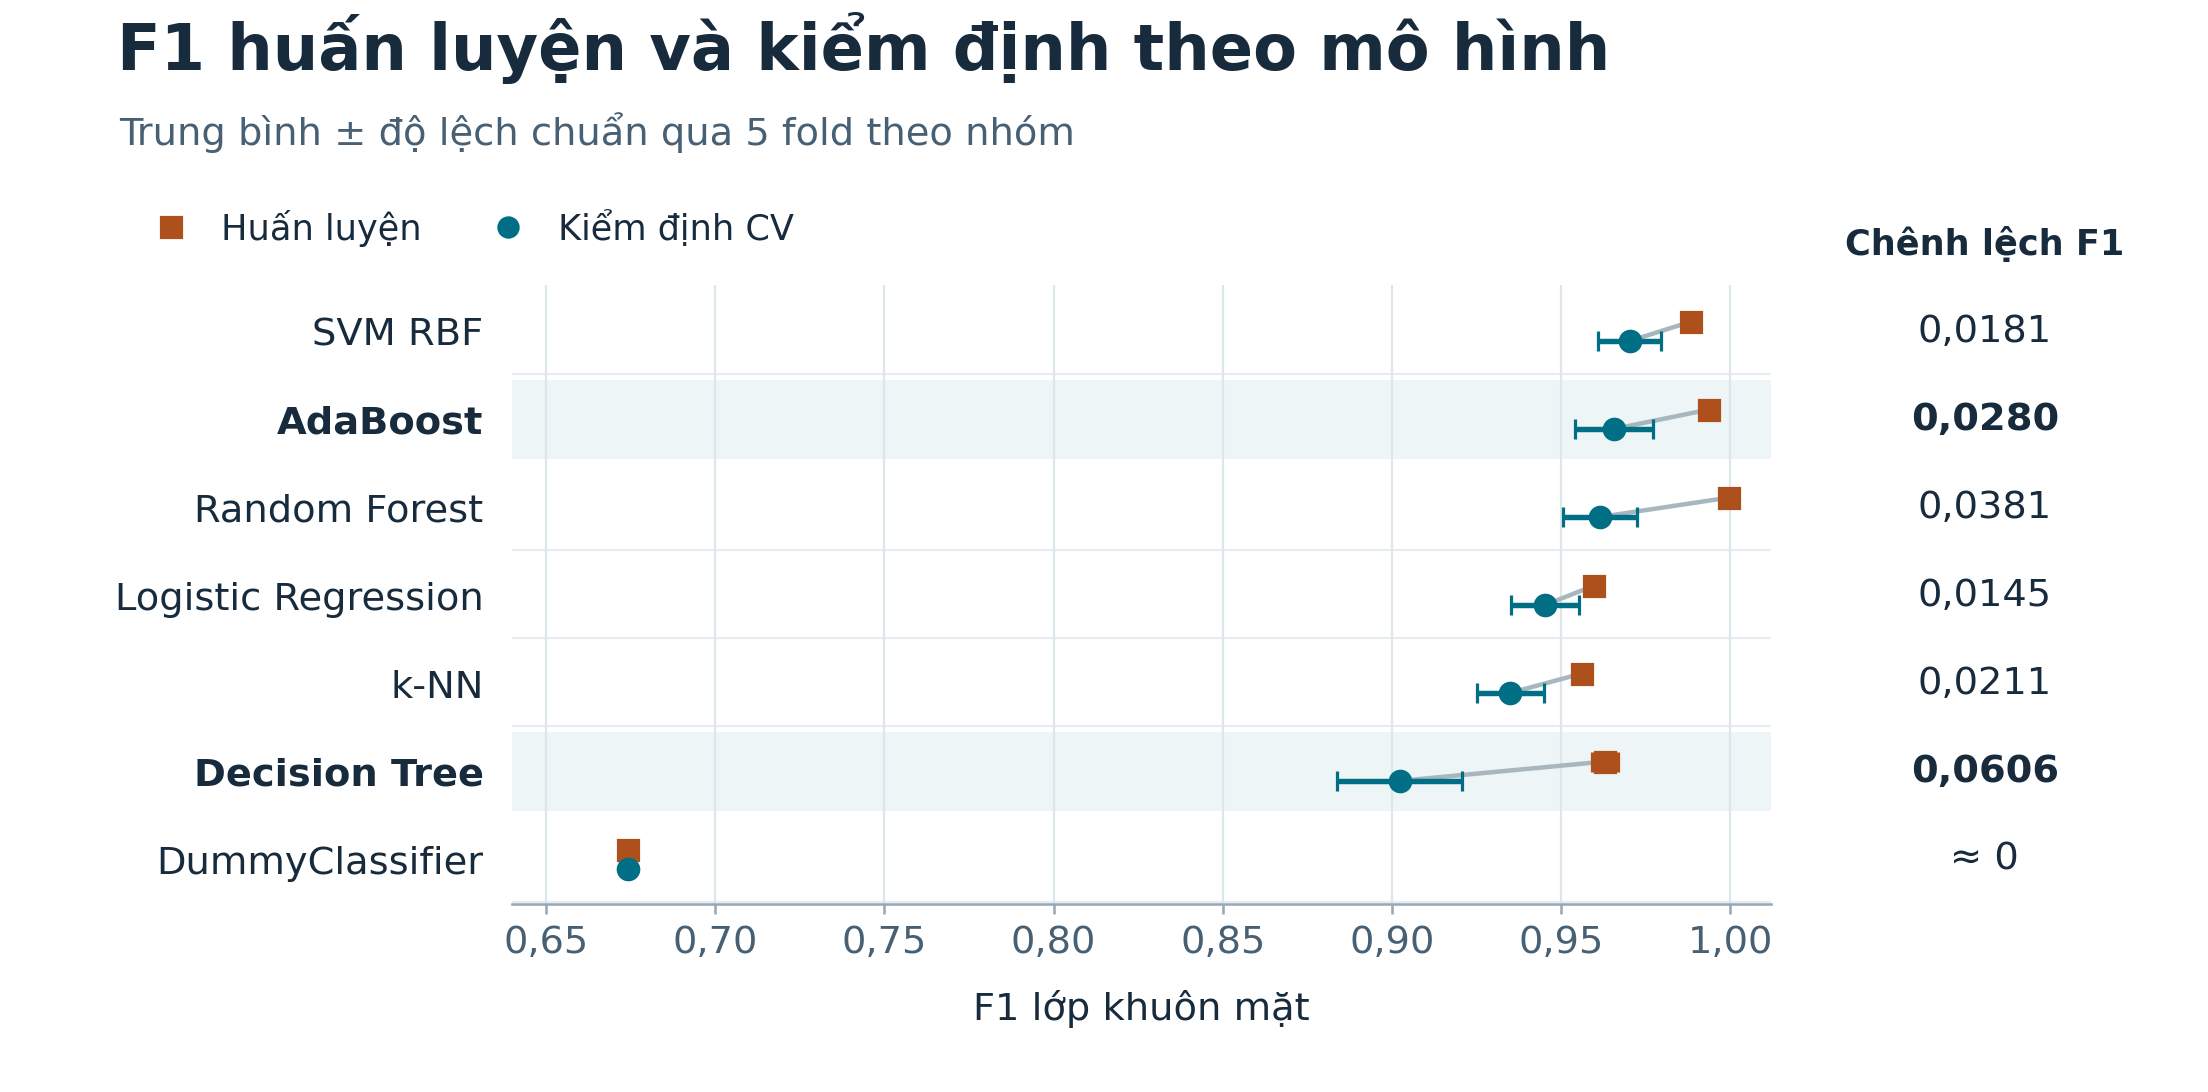
\includegraphics[width=\linewidth]{images/week8_f1_train_cv.png}
    \caption{So sánh $F_1$ huấn luyện và kiểm định trong năm fold.
    Thanh sai số biểu diễn một độ lệch chuẩn. Cột bên phải là chênh lệch
    giữa hai giá trị trung bình.}
    \label{fig:week8_f1_train_cv}
\end{figure}

\paragraph{Chênh lệch giữa huấn luyện và kiểm định.}
Decision Tree có $F_1$ trung bình giảm từ $0{,}9629$ xuống $0{,}9024$,
với chênh lệch $0{,}0606$, lớn nhất trong sáu mô hình học từ đặc trưng.
Độ lệch chuẩn trên các fold kiểm định của cây cũng cao nhất, bằng
$0{,}0185$. Trong các dự đoán ngoài fold, cây nhận nhầm 144 ảnh nền là
khuôn mặt và bỏ sót 109 ảnh khuôn mặt. Các số liệu cho thấy cấu hình
hiện tại khớp phần huấn luyện tốt hơn phần kiểm định và có kết quả
dao động nhiều hơn giữa các fold.

\paragraph{Chi phí huấn luyện của AdaBoost.}
Trong phép đo tuần 6, AdaBoost cần trung bình $8{,}89$ giây mỗi fold
để huấn luyện trên các véc-tơ Haar-like đã trích xuất, cao nhất trong
sáu mô hình khảo sát. Mô hình đạt $F_1$ kiểm định $0{,}9656$ và phát
sinh 50 lỗi báo nhầm nền, 38 lỗi bỏ sót mặt trên các dự đoán ngoài fold.
Chất lượng dự đoán và thời gian huấn luyện là hai đại lượng cần theo dõi
khi giảm số đặc trưng đầu vào.

\paragraph{Đề xuất giải pháp cải tiến.}
Bảng~\ref{tab:week8_limitations_solutions} liên hệ mỗi hạn chế với một
thay đổi có thể kiểm chứng trên cùng dữ liệu và cùng các fold.

\begin{table}[htbp]
    \centering
    \small
    \caption{Hạn chế của mô hình ban đầu và giải pháp đề xuất}
    \label{tab:week8_limitations_solutions}
    \begin{tabularx}{\linewidth}{
        @{}>{\raggedright\arraybackslash}p{0.29\linewidth}
        >{\raggedright\arraybackslash}X@{}
    }
        \toprule
        \textbf{Hạn chế} & \textbf{Giải pháp và cơ sở} \\
        \midrule
        AdaBoost có thời gian huấn luyện cao trong phép đo tuần 6.
        &
        Thử chọn 128 trong 258 đặc trưng Haar-like bằng
        \texttt{SelectKBest} với \texttt{f\_classif}. Cách này xếp hạng
        từng đặc trưng theo chênh lệch giữa hai lớp so với độ phân tán
        trong từng lớp, đồng thời giảm số biến mà cây yếu xem xét.
        Bộ chọn nằm trong \texttt{Pipeline} và chỉ học từ phần huấn luyện
        của mỗi fold. Đối chiếu $F_1$, Recall, FPR và thời gian huấn luyện
        với cấu hình dùng đủ 258 đặc trưng.
        \\
        \addlinespace
        Decision Tree có chênh lệch $F_1$ huấn luyện và kiểm định
        lớn, đồng thời dao động nhiều giữa các fold.
        &
        Khảo sát \texttt{max\_depth} và \texttt{min\_samples\_leaf}
        bằng kiểm định chéo theo nhóm. Giới hạn độ sâu và tăng số mẫu
        tối thiểu tại lá có thể hạn chế các phép chia dựa trên quá ít
        mẫu. Đánh giá tác động bằng $F_1$ kiểm định, độ lệch chuẩn qua
        các fold và chênh lệch $F_1$ huấn luyện so với kiểm định.
        \\
        \bottomrule
    \end{tabularx}
\end{table}

Hai giải pháp trên là giả thuyết thực nghiệm. Đợt so sánh đầu tiên
giữ nguyên cấu hình AdaBoost để đo riêng tác động của việc chọn
đặc trưng.

\subsection{Cải tiến dữ liệu và đặc trưng}
\label{subsec:week8_selectkbest}

Nhóm khảo sát việc giảm số đặc trưng Haar-like đầu vào của AdaBoost
từ 258 xuống 128 bằng \texttt{SelectKBest} với hàm \texttt{f\_classif}.
Giá trị $k=128$ được ấn định trước khi chạy. Cả hai cấu hình AdaBoost
dùng tối đa 100 cây quyết định với độ sâu tối đa bằng 1 cho mỗi cây
và tốc độ học bằng $1{,}0$. Cả hai được đánh giá trên cùng năm fold
theo nhóm của 2.511 ảnh con thuộc tập huấn luyện.

Ở từng fold, bộ chọn đặc trưng nằm trước AdaBoost trong \texttt{Pipeline}.
Bước này tính điểm $F$ từ phần huấn luyện của fold, chọn 128 cột có
điểm cao nhất rồi áp dụng đúng danh sách cột đó cho phần kiểm định.
Mỗi cấu hình được huấn luyện lại từ đầu cho từng fold, tổng cộng
10 lượt huấn luyện. Nhãn dự đoán lấy từ \texttt{predict()}, còn ROC-AUC
được tính từ điểm \texttt{decision\_function()}. Cấu hình dùng đủ 258
đặc trưng tái lập cả 2.511 nhãn và điểm dự đoán ngoài fold của tuần 6.

Bảng~\ref{tab:week8_selectkbest_results} trình bày trung bình và độ lệch
chuẩn ($\mathrm{ddof}=0$) qua năm fold. Hai dòng FP và FN cộng số lỗi
từ dự đoán ngoài fold, mỗi ảnh xuất hiện đúng một lần trong mỗi cấu hình.

\begin{table}[htbp]
    \centering
    \small
    \caption{Tác động của việc chọn đặc trưng đối với AdaBoost}
    \label{tab:week8_selectkbest_results}
    \begin{tabularx}{\linewidth}{@{}Xrr@{}}
        \toprule
        \textbf{Chỉ số} & \textbf{Dùng 258 đặc trưng} & \textbf{Chọn 128 đặc trưng} \\
        \midrule
        $F_1$ lớp khuôn mặt & $0{,}9656 \pm 0{,}0116$ & $0{,}9600 \pm 0{,}0111$ \\
        Recall (\%) & $97{,}02 \pm 1{,}93$ & $96{,}16 \pm 2{,}05$ \\
        FPR (\%) & $4{,}05 \pm 1{,}08$ & $4{,}30 \pm 1{,}37$ \\
        ROC-AUC & $0{,}9930 \pm 0{,}0037$ & $0{,}9927 \pm 0{,}0035$ \\
        Thời gian huấn luyện (giây/fold) & $8{,}92 \pm 0{,}32$ & $4{,}46 \pm 0{,}09$ \\
        Tổng lỗi báo nhầm nền (FP) & 50 & 53 \\
        Tổng lỗi bỏ sót mặt (FN) & 38 & 49 \\
        \bottomrule
    \end{tabularx}
\end{table}

Chọn 128 đặc trưng giảm thời gian huấn luyện trung bình khoảng
$50{,}0\%$. Thời gian này đo toàn bộ lệnh \texttt{fit}, gồm cả bước
chọn đặc trưng, trên ma trận Haar-like đã trích xuất. $F_1$ trung bình
giảm khoảng $0{,}0056$, với hai fold tăng và ba fold giảm. Recall giảm
$0{,}86$ điểm phần trăm và FPR tăng $0{,}25$ điểm phần trăm. Trên toàn
bộ dự đoán ngoài fold, cấu hình 128 đặc trưng có thêm 3 FP và 11 FN.

Có 118 đặc trưng được chọn ở cả năm fold. Danh sách thu được từ cả năm
fold có 137 đặc trưng phân biệt, cho thấy một phần danh sách thay đổi theo
mẫu huấn luyện. Bộ lọc xếp hạng từng cột riêng lẻ, vì vậy các cột bị bỏ
vẫn có thể hữu ích khi kết hợp trong mô hình. Với mục tiêu duy trì
chất lượng dự đoán trên năm fold đã xét, nhóm giữ cấu hình 258 đặc trưng
làm mốc tham chiếu cho AdaBoost ở các bước tiếp theo.

\subsection{Thử nghiệm thuật toán hoặc cấu hình khác}
\label{subsec:week8_dt_depth}

Nhóm khảo sát ảnh hưởng của độ sâu tối đa đến độ phức tạp và chất lượng
dự đoán của Decision Tree. Cấu hình tuần 6 đặt \texttt{max\_depth=5}.
Trong cấu hình khảo sát, nhóm giảm tham số này xuống 3. Cả hai cấu hình
dùng 258 đặc trưng Haar-like, \texttt{min\_samples\_leaf=2}
và \texttt{random\_state=42}.

Hai cấu hình được đánh giá trên cùng năm fold theo nhóm của 2.511 ảnh con
thuộc tập huấn luyện. Mỗi cấu hình được huấn luyện lại trên phần train
của từng fold, tổng cộng 10 lượt. Nhãn lấy từ \texttt{predict()}, còn
ROC-AUC được tính từ xác suất của lớp khuôn mặt. Cấu hình độ sâu 5
khớp cả 2.511 nhãn và xác suất ngoài fold đã lưu ở tuần 6.

Bảng~\ref{tab:week8_dt_depth_results} tổng hợp kết quả qua năm fold.
Chênh lệch $F_1$ được tính bằng $F_1$ huấn luyện trừ $F_1$ kiểm định trên
từng fold. Trừ hai dòng tổng FP và FN, các giá trị trong bảng được trình
bày dưới dạng trung bình và độ lệch chuẩn với $\mathrm{ddof}=0$.

\begin{table}[htbp]
    \centering
    \small
    \caption{Ảnh hưởng của độ sâu tối đa đối với Decision Tree}
    \label{tab:week8_dt_depth_results}
    \begin{tabularx}{\linewidth}{@{}Xrr@{}}
        \toprule
        \textbf{Chỉ số} & \textbf{Độ sâu 5} & \textbf{Độ sâu 3} \\
        \midrule
        $F_1$ huấn luyện & $0{,}9629 \pm 0{,}0039$ & $0{,}9165 \pm 0{,}0047$ \\
        $F_1$ kiểm định & $0{,}9024 \pm 0{,}0185$ & $0{,}8921 \pm 0{,}0231$ \\
        Chênh lệch $F_1$ & $0{,}0606 \pm 0{,}0223$ & $0{,}0244 \pm 0{,}0263$ \\
        Recall kiểm định (\%) & $91{,}46 \pm 1{,}77$ & $91{,}85 \pm 2{,}60$ \\
        FPR kiểm định (\%) & $11{,}67 \pm 2{,}75$ & $14{,}59 \pm 3{,}49$ \\
        ROC-AUC kiểm định & $0{,}9320 \pm 0{,}0246$ & $0{,}9373 \pm 0{,}0174$ \\
        Số lá & $30{,}2 \pm 0{,}7$ & $8{,}0 \pm 0{,}0$ \\
        Thời gian huấn luyện (giây/fold) & $0{,}305 \pm 0{,}018$ & $0{,}179 \pm 0{,}003$ \\
        Tổng lỗi báo nhầm nền (FP) & 144 & 180 \\
        Tổng lỗi bỏ sót mặt (FN) & 109 & 104 \\
        \bottomrule
    \end{tabularx}
\end{table}

Khi giảm độ sâu xuống 3, số lá trung bình giảm từ $30{,}2$ xuống $8$.
Chênh lệch $F_1$ thu hẹp từ $0{,}0606$ xuống $0{,}0244$, chủ yếu do
$F_1$ trên phần huấn luyện giảm nhiều hơn $F_1$ trên phần kiểm định.
$F_1$ kiểm định giảm khoảng $0{,}0103$ và dao động nhiều hơn giữa các
fold. Kết quả này cho thấy cần xem đồng thời chất lượng kiểm định và
khoảng cách huấn luyện--kiểm định khi đánh giá độ phức tạp của cây.

Trong 2.511 dự đoán ngoài fold, cấu hình độ sâu 3 bỏ sót ít hơn 5 ảnh
khuôn mặt và báo nhầm thêm 36 ảnh nền. ROC-AUC trung bình tăng nhẹ,
trong khi $F_1$ tại quy tắc dự đoán mặc định giảm. ROC-AUC dựa trên
thứ tự của các điểm dự đoán, còn $F_1$ dựa trên nhãn dự đoán ở một
quy tắc cụ thể. Với ưu tiên $F_1$
cao và tỷ lệ báo nhầm thấp trên các fold đã xét, cấu hình độ sâu 5
được giữ làm mốc đối chiếu cho bước tìm kiếm siêu tham số.

\subsection{Tối ưu hóa siêu tham số}
\label{subsec:week8_dt_tuning}

Nhóm dùng \texttt{GridSearchCV} để khảo sát hai siêu tham số
quyết định độ phức tạp của Decision Tree trên 258 đặc trưng Haar-like.
\texttt{max\_depth} giới hạn độ sâu của cây và được thử ở các mức
$\{3,5,7\}$, bao quanh cấu hình độ sâu 5 của tuần 6.
\texttt{min\_samples\_leaf} quy định số mẫu tối thiểu trong một lá
và được thử ở các mức $\{2,5,10\}$ để đánh giá ảnh hưởng của việc
tăng số mẫu hỗ trợ mỗi dự đoán tại lá. Cây sử dụng
\texttt{random\_state=42} và bước tiền xử lý \texttt{passthrough}
trong \texttt{Pipeline}.

Kiểm định chéo lồng nhau được thực hiện trên 2\,511 mẫu huấn luyện.
Vòng ngoài giữ đúng 5 fold theo nhóm đã lưu ở tuần 6.
Trong phần huấn luyện của mỗi fold ngoài, nhóm dùng
\texttt{StratifiedGroupKFold} với 3 fold, \texttt{shuffle=True}
và \texttt{random\_state=42}. Nhóm được xác định theo danh tính người
đối với mẫu face và theo ảnh nền gốc đối với mẫu non-face.
Số nhóm giao nhau giữa phần huấn luyện và phần kiểm định bằng 0
ở cả 5 lần chia ngoài và 15 lần chia trong.

Mỗi fold ngoài thử đủ 9 tổ hợp trên 3 fold trong.
\texttt{GridSearchCV} chọn tổ hợp có $F_1$ trung bình của lớp face
cao nhất rồi huấn luyện lại trên toàn bộ phần huấn luyện của fold ngoài
với \texttt{refit=True}. Mô hình thu được dự đoán trên phần kiểm định
của fold ngoài bằng \texttt{Pipeline.predict()}. ROC-AUC được tính từ
xác suất ước lượng của lớp face. Thí nghiệm gồm
$5 \times (9 \times 3 + 1) = 140$ lượt huấn luyện.

\begin{table}[htbp]
  \centering
  \small
  \caption{Siêu tham số được chọn và kết quả của Decision Tree
    trong kiểm định chéo lồng nhau.}
  \label{tab:week8_dt_best_grid}
  \begin{tabular}{@{}ccccc@{}}
    \toprule
    \textbf{Fold ngoài} & \texttt{max\_depth}
    & \texttt{min\_samples\_leaf}
    & $F_1$ \textbf{vòng trong} & $F_1$ \textbf{vòng ngoài} \\
    \midrule
    1 & 5 & 5 & $0{,}9120$ & $0{,}8750$ \\
    2 & 7 & 2 & $0{,}8993$ & $0{,}9133$ \\
    3 & 3 & 2 & $0{,}8954$ & $0{,}9243$ \\
    4 & 7 & 5 & $0{,}9055$ & $0{,}9084$ \\
    5 & 5 & 5 & $0{,}9028$ & $0{,}8845$ \\
    \midrule
    \multicolumn{4}{@{}l}{\textbf{Trung bình $\pm$ độ lệch chuẩn vòng ngoài}}
    & $0{,}9011 \pm 0{,}0184$ \\
    \bottomrule
  \end{tabular}
\end{table}

Bảng~\ref{tab:week8_dt_best_grid} ghi lại cấu hình được chọn riêng
cho từng fold ngoài. Ở fold 3, ba cấu hình độ sâu 3 cùng đạt
$F_1$ vòng trong cao nhất. \texttt{GridSearchCV} chọn tổ hợp đầu tiên
là $(3,2)$. Trên 5 fold ngoài, Recall trung bình
đạt $91{,}62\%$, FPR đạt $12{,}15\%$ và ROC-AUC đạt $0{,}9208$.
Mã chạy và các bảng kết quả được lưu trong thư mục \texttt{week8/}
với tiền tố \texttt{week8\_tc5\_} cho các tệp CSV.

\section{So sánh trước và sau cải tiến}
\label{sec:week8_ablation}

Các cấu hình trong Bảng~\ref{tab:week8_comparison} dùng cùng
2\,511 mẫu, cùng 5 fold ngoài theo nhóm và cùng quy tắc dự đoán
\texttt{Pipeline.predict()}. Mỗi ảnh đóng góp một dự đoán ngoài fold
cho từng cấu hình. Các chỉ số được tính trên phần kiểm định của từng
fold rồi lấy trung bình. Độ lệch chuẩn của $F_1$ được tính với mẫu số 5.
Cột FP và FN là tổng số lỗi tương ứng trên toàn bộ dự đoán ngoài fold.

\begin{table}[htbp]
  \centering
  \small
  \caption{So sánh các cấu hình trước và sau cải tiến trên cùng 5 fold.}
  \label{tab:week8_comparison}
  \begin{tabularx}{\linewidth}{@{}>{\raggedright\arraybackslash}X c r r r r r@{}}
    \toprule
    \textbf{Cấu hình}
    & $F_1$ \textbf{(TB $\pm$ ĐLC)}
    & \textbf{Recall (\%)}
    & \textbf{FPR (\%)}
    & \textbf{ROC-AUC}
    & \textbf{FP}
    & \textbf{FN} \\
    \midrule
    AdaBoost, 258 đặc trưng
    & $0{,}9656 \pm 0{,}0116$ & $97{,}02$ & $4{,}05$ & $0{,}9930$ & 50 & 38 \\
    AdaBoost, chọn 128 đặc trưng
    & $0{,}9600 \pm 0{,}0111$ & $96{,}16$ & $4{,}30$ & $0{,}9927$ & 53 & 49 \\
    \addlinespace
    Decision Tree, độ sâu 5
    & $0{,}9024 \pm 0{,}0185$ & $91{,}46$ & $11{,}67$ & $0{,}9320$ & 144 & 109 \\
    Decision Tree, độ sâu 3
    & $0{,}8921 \pm 0{,}0231$ & $91{,}85$ & $14{,}59$ & $0{,}9373$ & 180 & 104 \\
    Decision Tree, Grid Search lồng nhau
    & $0{,}9011 \pm 0{,}0184$ & $91{,}62$ & $12{,}15$ & $0{,}9208$ & 150 & 107 \\
    \bottomrule
  \end{tabularx}
\end{table}

\begin{itemize}
  \item \textbf{Lựa chọn đặc trưng cho AdaBoost.}
    Bổ sung \texttt{SelectKBest} vào Pipeline và giữ nguyên cấu hình
    AdaBoost giúp giảm thời gian huấn luyện trung bình từ $8{,}92$
    xuống $4{,}46$ giây mỗi fold trong cùng thí nghiệm.
    $F_1$ giảm $0{,}0056$ và số mẫu face bị bỏ sót tăng từ 38 lên 49.
    Cấu hình 128 đặc trưng đánh đổi một phần khả năng phát hiện
    để giảm chi phí huấn luyện.

  \item \textbf{Giảm độ sâu của Decision Tree.}
    Trên 258 đặc trưng và với \texttt{min\_samples\_leaf=2},
    giảm độ sâu tối đa từ 5 xuống 3 làm số lá trung bình giảm từ
    $30{,}2$ xuống $8{,}0$. Số bỏ sót giảm 5, nhưng số báo nhầm
    tăng 36, tương ứng FPR tăng $2{,}92$ điểm phần trăm.
    $F_1$ trung bình giảm $0{,}0103$.

  \item \textbf{Tối ưu siêu tham số của Decision Tree.}
    So với cây độ sâu 5, quy trình chọn cấu hình theo $F_1$
    ở vòng trong cho $F_1$ vòng ngoài cao hơn ở 2 trong 5 fold.
    Trung bình $F_1$ giảm $0{,}0013$, FPR tăng $0{,}48$ điểm phần trăm
    và ROC-AUC giảm $0{,}0112$. Chênh lệch $F_1$ giữa phần huấn luyện
    và phần kiểm định chỉ giảm từ $0{,}0606$ xuống $0{,}0603$.
    Kết quả cho thấy việc chọn cấu hình theo $F_1$ trong phạm vi
    lưới đã thử chưa đem lại lợi ích nhất quán trên các fold ngoài.
\end{itemize}

Trong các cấu hình ở Bảng~\ref{tab:week8_comparison},
hai cấu hình AdaBoost cùng đạt các mục tiêu trung bình qua 5 fold
về Recall, FPR và ROC-AUC. AdaBoost với 258 đặc trưng có $F_1$
và Recall cao hơn bản chọn 128 đặc trưng, đồng thời có ít lỗi FP
và FN hơn. Đây là kết quả trên các cửa sổ ảnh xám $24 \times 24$
thuộc tập huấn luyện, được đánh giá bằng dự đoán ngoài fold.

\section{Khả năng tổng quát hóa và lựa chọn mô hình cuối}

\subsection{Khả năng tổng quát hóa}
\label{subsec:week8_generalization}

Nhóm chọn AdaBoost với 258 đặc trưng Haar-like dựa trên kết quả
kiểm định chéo theo nhóm. Để đánh giá cấu hình đã chọn, nhóm
huấn luyện lại Pipeline của tuần 6 trên toàn bộ 2\,511 mẫu train.
Cấu hình dùng cây quyết định độ sâu 1, tối đa 100 cây yếu,
\texttt{learning\_rate=1.0} và \texttt{random\_state=42}.
Số nhóm giao nhau giữa tập huấn luyện và tập kiểm tra bằng 0.

Nhóm đánh giá lại trên cùng 538 mẫu test giữ riêng đã dùng
ở tuần 6. Kiểm định chéo và đánh giá test cùng dùng
\texttt{Pipeline.predict()} để dự đoán nhãn. ROC-AUC được
tính từ điểm quyết định của AdaBoost. Bảng~\ref{tab:week8_cv_vs_test}
trình bày trung bình và độ lệch chuẩn (mẫu số 5) của các chỉ số
qua 5 fold, cùng kết quả trên tập test.

\begin{table}[htbp]
  \centering
  \small
  \caption{So sánh AdaBoost 258 đặc trưng trên 5 fold
    kiểm định chéo và tập test giữ riêng.}
  \label{tab:week8_cv_vs_test}
  \begin{tabular}{@{}lcc@{}}
    \toprule
    \textbf{Chỉ số} & \textbf{CV (TB $\pm$ ĐLC)} & \textbf{Test (538 mẫu)} \\
    \midrule
    $F_1$ & $0{,}9656 \pm 0{,}0116$ & $0{,}9551$ \\
    Recall (DR, \%) & $97{,}02 \pm 1{,}93$ & $96{,}30$ \\
    FPR (\%) & $4{,}05 \pm 1{,}08$ & $4{,}41$ \\
    ROC-AUC & $0{,}9930 \pm 0{,}0037$ & $0{,}9935$ \\
    \bottomrule
  \end{tabular}
\end{table}

Trong 243 mẫu face của tập test, mô hình nhận đúng 234 mẫu
và bỏ sót 9 mẫu. Trong 295 mẫu non-face, mô hình nhận đúng
282 mẫu và báo nhầm 13 mẫu. So với trung bình CV, $F_1$
trên test thấp hơn $0{,}0105$, Recall giảm $0{,}73$ điểm phần trăm
và FPR tăng $0{,}36$ điểm phần trăm. Cả ba chỉ số mục tiêu
trên test vẫn đạt các mức kỳ vọng của đề tài, gồm Recall
$\geq 90\%$, FPR $\leq 5\%$ và ROC-AUC $\geq 0{,}90$.
Các nhãn dự đoán của 538 mẫu khớp với kết quả AdaBoost
mặc định đã lưu ở tuần 6.

\subsubsection{Độ ổn định qua các fold}

\begin{figure}[htbp]
  \centering
  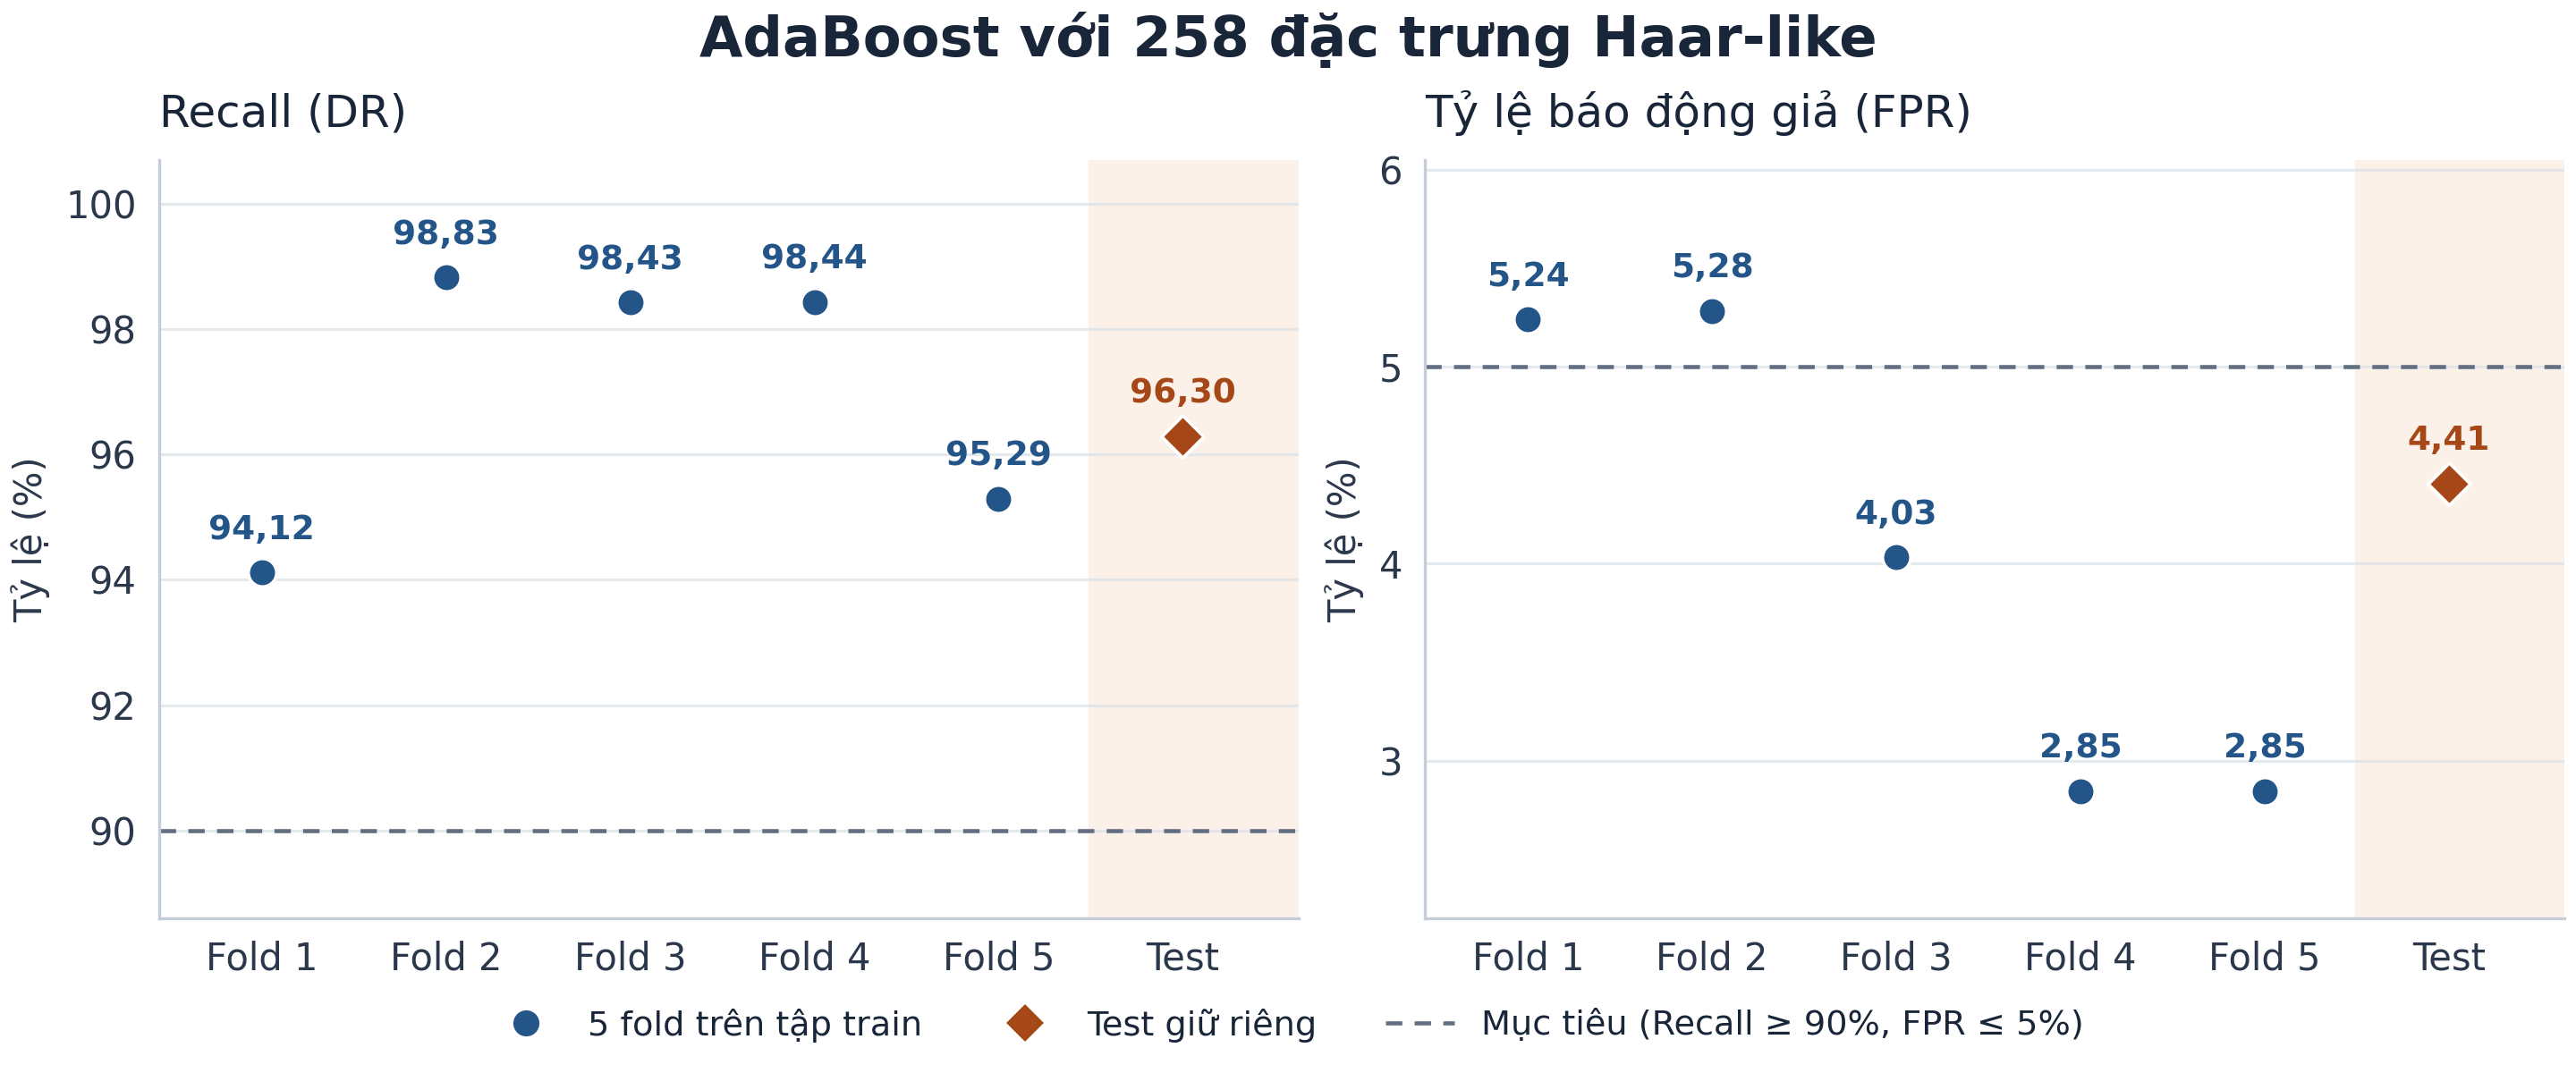
\includegraphics[width=\linewidth]{images/week8_adaboost_cv_vs_test.png}
  \caption{Recall và FPR của AdaBoost theo từng fold và trên tập test.
    Đường nét đứt biểu diễn mức mục tiêu của mỗi chỉ số.}
  \label{fig:week8_adaboost_cv_vs_test}
\end{figure}

Hình~\ref{fig:week8_adaboost_cv_vs_test} cho thấy Recall của
cả năm fold đều vượt $90\%$, dao động từ $94{,}12\%$ đến
$98{,}83\%$. FPR dao động từ $2{,}85\%$ đến $5{,}28\%$.
Hai fold đầu có FPR lần lượt là $5{,}24\%$ và $5{,}28\%$.
Vì vậy, mức FPR trung bình $4{,}05\%$ đi kèm với hai lần
chia vượt mục tiêu $5\%$. $F_1$ trên test nằm trong khoảng
$0{,}9449$ đến $0{,}9786$ quan sát được qua các fold.
Các kết quả này áp dụng cho phân loại cửa sổ ảnh xám
$24 \times 24$ pixel. Việc đánh giá vị trí khuôn mặt trên ảnh
đầy đủ cần dữ liệu có nhãn khung bao.

\subsection{Lựa chọn mô hình cuối cùng}
\label{subsec:week8_final_model_choice}

Trong các cấu hình đạt cả ba mục tiêu khi xét trung bình CV,
AdaBoost 258 đặc trưng có Recall cao nhất, đạt $97{,}02\%$.
SVM RBF có $F_1$ cao hơn ($0{,}9703$ so với $0{,}9656$)
và FPR thấp hơn ($2{,}27\%$ so với $4{,}05\%$).
Chọn AdaBoost ưu tiên giảm số mẫu face bị bỏ sót,
với Recall cao hơn SVM RBF $0{,}71$ điểm phần trăm
và FPR cao hơn $1{,}78$ điểm phần trăm trên cùng các fold.

Trong phép kiểm định chéo tuần 6 trên cùng máy, thời gian
huấn luyện trung bình mỗi fold của AdaBoost và SVM RBF
lần lượt là $8{,}89$ và $0{,}16$ giây. Thời gian dự đoán
một fold gồm 501--503 mẫu lần lượt là $34{,}1$ và $75{,}0$
mili giây. Với AdaBoost, có thể kiểm tra đặc trưng Haar-like
và ngưỡng tách ở từng cây yếu. Giải thích quyết định cuối
cần xét đóng góp tổng hợp của các cây. Nhóm chọn giữ
258 đặc trưng vì cấu hình này có Recall cao hơn biến thể
128 đặc trưng với cùng thiết lập AdaBoost.

\section{Kết luận chương 3}


% =====================================================================
%  KẾT LUẬN
% =====================================================================
\unnumberedchapter{KẾT LUẬN VÀ HƯỚNG PHÁT TRIỂN}

\section*{1. Kết quả đạt được}


\section*{2. Hạn chế}


\section*{3. Hướng phát triển}


% =====================================================================
%  TÀI LIỆU THAM KHẢO
%  Quy ước: tài liệu tiếng Việt trước, tiếng nước ngoài sau; xếp theo
%  ABC của tên (tiếng Việt) hoặc họ (tiếng nước ngoài) tác giả.
% =====================================================================
\begin{thebibliography}{99}
\setlength{\itemsep}{2pt}

\bibitem{lananh}
Nguyễn Thị Lan Anh, ``Cải thiện kết quả dự đoán điểm thi của sinh viên
bằng Máy học với sự hỗ trợ của R''.

\bibitem{tuananh2024}
Nguyễn Tuấn Anh (2024), ``Ứng dụng mô hình học máy vào trong dự đoán kết
quả học tập của sinh viên tại ICTU'', \textit{Tạp chí Khoa học và Công nghệ
Đại học Thái Nguyên}.

\bibitem{hai2017}
Trương Thị Hải, Nguyễn Thái Nghe, Huỳnh Xuân Hiệp (2017), ``Giải pháp hỗ trợ
sinh viên lập kế hoạch học tập dựa trên tiếp cận tập thô'',
\textit{Kỷ yếu Hội thảo, NXB Khoa học Tự nhiên và Công nghệ}.

\bibitem{thuan2022}
Trần Bá Thuấn (2022), ``Ứng dụng machine learning dự báo sinh viên diện cảnh
báo học tập tại Trường Đại học Kinh tế Huế'', \textit{Tạp chí Khoa học Quản
lý và Kinh tế, Trường Đại học Kinh tế, Đại học Huế}, số 21.

\bibitem{thuy2023}
Nguyễn Văn Thủy (2023), ``Sử dụng các mô hình Machine Learning dự đoán tình
trạng sinh viên tốt nghiệp đúng hạn'', \textit{Tạp chí Khoa học Đào tạo
Ngân hàng}, số 225(8), tr.~52--64.

\bibitem{alquraishi2021}
M.~AlQuraishi (2021), ``Machine learning in protein structure prediction'',
\textit{Current Opinion in Chemical Biology}, vol.~65, pp.~1--8.

\bibitem{breiman2001}
L.~Breiman (2001), ``Random forests'', \textit{Machine Learning}, vol.~45,
no.~1, pp.~5--32.

\bibitem{chen2016}
T.~Chen, C.~Guestrin (2016), ``XGBoost: A scalable tree boosting system'',
in \textit{Proceedings of the 22nd ACM SIGKDD International Conference on
Knowledge Discovery and Data Mining}, pp.~785--794.

\bibitem{pedregosa2011}
F.~Pedregosa \textit{et al.} (2011), ``Scikit-learn: Machine learning in
Python'', \textit{Journal of Machine Learning Research}, vol.~12,
pp.~2825--2830.

\end{thebibliography}

% =====================================================================
%  PHỤ LỤC
% =====================================================================
\appendix
\renewcommand{\bmchapname}{Phụ lục}
\addtocontents{toc}{\protect\renewcommand{\protect\tocchapname}{\appendixname}}

% Thay noi dung Phu luc A cu bang toan bo noi dung tep nay.
% Giu lenh \appendix da co trong main.tex; khong them \appendix lan nua.
% Giu lai Phu luc B nam sau phan nay.

\chapter{Hướng dẫn cài đặt và chạy chương trình}
\label{pl:huongdan}

Phụ lục hướng dẫn chạy notebook thực nghiệm tuần 6 và giao diện minh họa
bộ phân loại cửa sổ ảnh của đề tài. Chương trình sử dụng dữ liệu đã xử lý
và các mô hình của nhóm; mỗi ảnh con mức xám có kích thước
$24 \times 24$ điểm ảnh được biểu diễn bằng 258 đặc trưng Haar-like.

\section{Yêu cầu môi trường}

\begin{itemize}
    \item Môi trường đã sử dụng: Windows 64-bit, Python 3.12.4;
    có thể thao tác bằng Terminal trong Antigravity, Visual Studio Code
    hoặc PowerShell.
    \item Các thư viện thực nghiệm được ghi trong
    \path{requirements-week6.txt}, gồm NumPy 2.4.6, pandas 3.0.5,
    Scikit-learn 1.9.1, SciPy 1.18.1, Matplotlib 3.11.1,
    Seaborn 0.13.2 và các thư viện hỗ trợ notebook.
    \item Giao diện sử dụng Streamlit, joblib và Pillow.
    Các phụ thuộc demo được cài bằng \path{requirements-demo.txt}.
    Khi nạp các mô hình đã lưu, sử dụng môi trường tương thích với
    môi trường xuất mô hình, đặc biệt là Scikit-learn 1.9.1.
    \item Sử dụng trình duyệt web để mở giao diện Streamlit;
    sử dụng Jupyter hoặc công cụ hỗ trợ notebook trong IDE để chạy
    tệp thực nghiệm.
\end{itemize}

\section{Chuẩn bị mã nguồn và dữ liệu}

Giải nén các gói \path{week6_review_bundle.zip} và
\path{week6_demo_bundle.zip} vào cùng một thư mục gốc dự án.
Thư mục này cần chứa:

\begin{itemize}
    \item Notebook \path{02_Week6_Training_FaceDetection.ipynb},
    các tệp hướng dẫn \path{README_WEEK6.md}, \path{README_DEMO.md}
    và hai tệp danh sách phụ thuộc.
    \item Mã demo: \path{app_demo.py}, \path{haar_extractor.py}
    và \path{train_export_demo.py}.
    \item Thư mục \path{data/processed/}, gồm ảnh
    \path{images_24x24.npy}, đặc trưng \path{haar_features.npy},
    nhãn \path{labels.npy}, \path{metadata.csv},
    \path{split_indices.npz}, \path{haar_dataset_splits.npz}
    và \path{data_dictionary_haar.csv}.
    \item Thư mục \path{models/demo/}, gồm bảy tệp mô hình
    \texttt{.joblib} và tệp \path{demo_metadata.json}.
    \item Thư mục \path{reports/tables/} chứa phân công fold,
    giao thức ngưỡng và các bảng kết quả;
    \path{reports/figures/} chứa các biểu đồ đã xuất.
\end{itemize}

Toàn bộ dữ liệu gồm 3.589 ảnh con: tập train có 2.511 mẫu,
validation có 540 mẫu và test có 538 mẫu. Giữ nguyên các tệp phân chia
và phân công fold để chạy lại theo đúng thiết kế thực nghiệm.

\section{Cài đặt các thư viện}

Mở Terminal tại thư mục gốc dự án. Ví dụ dưới đây sử dụng PowerShell
và đường dẫn trên máy thực nghiệm; trên máy khác, thay đường dẫn
bằng vị trí đã giải nén:

\begin{lstlisting}[language={},numbers=none]
cd "C:\Users\mrddd\Documents\FaceDetection_Week4"
python --version
python -m pip install -r requirements-week6.txt
python -m pip install -r requirements-demo.txt
\end{lstlisting}

Sử dụng cùng một trình thông dịch Python để cài thư viện và chạy chương
trình. Có thể kiểm tra phiên bản Scikit-learn bằng lệnh:

\begin{lstlisting}[language={},numbers=none]
python -c "import sklearn; print(sklearn.__version__)"
\end{lstlisting}

Đối với các mô hình đã được bàn giao, phiên bản Scikit-learn ghi nhận
trong thông tin xuất mô hình là \texttt{1.9.1}.

\section{Chạy notebook thực nghiệm tuần 6}

\begin{enumerate}
    \item Mở thư mục gốc dự án trong IDE hoặc Jupyter và mở
    \path{02_Week6_Training_FaceDetection.ipynb}.
    Thư mục làm việc của notebook phải là thư mục chứa
    \path{data/processed/} và \path{reports/}.
    \item Chọn kernel thuộc môi trường Python đã cài các thư viện ở trên.
    \item Chọn thao tác khởi động lại kernel và chạy toàn bộ các ô mã
    theo thứ tự từ trên xuống dưới
    (\textit{Restart Kernel and Run All Cells}).
    \item Kiểm tra các thông báo về kích thước dữ liệu, phân chia theo nhóm,
    kiểm định chéo, lựa chọn ngưỡng và bảng kết quả; sau đó lưu notebook
    để giữ lại đầu ra thực thi.
\end{enumerate}

Notebook sử dụng tập train để huấn luyện và kiểm định chéo 5 fold,
tập validation giữ riêng để lựa chọn ngưỡng, và tập test để đánh giá cuối
theo cấu hình, ngưỡng đã xác định từ train/validation.
Việc chạy lại phục vụ kiểm tra khả năng tái lập; kết quả test không được
dùng để lựa chọn lại cấu hình hoặc ngưỡng nhằm cải thiện số liệu đã báo cáo.
Các bảng và hình được lưu trong \path{reports/tables/}
và \path{reports/figures/}.

\section{Khởi chạy và thao tác trên giao diện demo}

Các mô hình đã fit được cung cấp sẵn trong \path{models/demo/}.
Để mở giao diện, chạy lệnh sau từ thư mục gốc dự án:

\begin{lstlisting}[language={},numbers=none]
python -m streamlit run app_demo.py
\end{lstlisting}

Nếu lần khởi chạy đầu tiên yêu cầu nhập email, có thể để trống và nhấn
\texttt{Enter}. Mở địa chỉ ở dòng \texttt{Local URL} do Terminal hiển thị,
thường là \url{http://localhost:8501}. Giữ Terminal hoạt động trong khi
sử dụng; nhấn \texttt{Ctrl + C} tại Terminal để dừng chương trình.

Đối với phiên bản minh họa phân loại ảnh con đã bàn giao,
thực hiện theo trình tự:

\begin{enumerate}
    \item Chọn thuật toán tại thanh bên; mặc định là AdaBoost.
    \item Chọn ảnh thuộc tập train bằng chỉ số dòng toàn cục,
    mã \texttt{source\_id} hoặc nút chọn ngẫu nhiên.
    Có thể lọc lớp face hoặc non-face để chọn mẫu minh họa.
    \item Nhấn nút dự đoán mẫu. Chương trình trích xuất 258 đặc trưng
    từ ảnh đã chọn và đưa vào Pipeline để tính nhãn dự đoán.
    Nhãn thực tế chỉ dùng để đối chiếu kết quả.
    \item Nhấn nút so sánh sáu mô hình để xem các nhãn dự đoán
    trên cùng một ảnh. Có thể bật thêm DummyClassifier làm mốc cơ sở.
    \item Khi sử dụng tùy chọn ngưỡng validation, kiểm tra thông tin
    mô hình và ngưỡng đi kèm. Nếu chưa xác nhận được sự tương ứng,
    tắt tùy chọn này để dùng phương thức \texttt{Pipeline.predict()}.
\end{enumerate}

Các mẫu train được sử dụng để minh họa thao tác và quá trình suy luận.
Kết quả trên những mẫu này không thay thế đánh giá trên validation/test
giữ riêng. Điểm quyết định hoặc xác suất ước lượng của một mẫu không
phải là chỉ số Accuracy của mô hình.

\section{Xuất lại mô hình khi cần}

Nếu cần tạo lại các tệp mô hình từ mã nguồn và dữ liệu đã bàn giao,
sử dụng đúng môi trường thực nghiệm và chạy:

\begin{lstlisting}[language={},numbers=none]
python train_export_demo.py
\end{lstlisting}

Script kiểm tra bộ trích xuất đặc trưng, fit các Pipeline trên
2.511 mẫu train và lưu mô hình vào \path{models/demo/}.
Chỉ thực hiện bước này khi cần tái tạo mô hình; các lần mở demo thông thường
sử dụng trực tiếp các tệp đã lưu.
Sau khi xuất lại, cần đối chiếu mô hình trước khi áp dụng ngưỡng
validation đi kèm, vì ngưỡng phụ thuộc vào điểm số của mô hình cụ thể.

\section{Kiểm tra khi chương trình gặp lỗi}

\begin{itemize}
    \item \textbf{Thiếu thư viện:} kiểm tra trình thông dịch hoặc kernel
    đang sử dụng, rồi cài phụ thuộc bằng \texttt{python -m pip}
    trong đúng môi trường đó.
    \item \textbf{Không tìm thấy dữ liệu hoặc tệp mô hình:}
    đối chiếu cấu trúc thư mục ở trên, vị trí giải nén và thư mục làm việc.
    Các tệp mô hình cần nằm trong \path{models/demo/}.
    \item \textbf{Cảnh báo khác phiên bản khi nạp mô hình:}
    đối chiếu phiên bản thư viện với \path{demo_metadata.json}
    và môi trường đã dùng để xuất mô hình.
    \item \textbf{Không mở được giao diện:} đọc thông báo trong Terminal
    và truy cập đúng \texttt{Local URL} của phiên chạy hiện tại.
    Nếu cổng mặc định đang được sử dụng, có thể chọn cổng khác:
\end{itemize}

\begin{lstlisting}[language={},numbers=none]
python -m streamlit run app_demo.py --server.port 8502
\end{lstlisting}

\paragraph{Phạm vi phiên bản được hướng dẫn.}
Gói demo được đối chiếu trong phụ lục này minh họa tầng phân loại
cửa sổ ảnh $24 \times 24$. Hướng dẫn tự động định vị và vẽ khung khuôn mặt
trên ảnh đầy đủ sẽ được bổ sung khi mô-đun phát hiện tương ứng được
hoàn thiện và kiểm tra. Các chỉ số thực nghiệm hiện có cần được diễn giải
đúng ở mức phân loại cửa sổ ảnh.

\chapter{Nhật ký đóng góp của các thành viên}
\label{pl:nhatky}
\begin{table}[H]
  \centering
  \caption{Nhật ký công việc theo tuần}
  \label{tab:nhatky}
  \small
  \begin{tabularx}{\textwidth}{
    >{\centering\arraybackslash}p{0.8cm}
    >{\centering\arraybackslash}p{1.8cm}
    p{2.5cm}
    X}
    \toprule
    \textbf{Tuần} & \textbf{Ngày} & \textbf{Thành viên} & \textbf{Công việc / commit} \\
    \midrule

    1 & 24/10/2026 & \svAten &
    Tìm hiểu đề tài phát hiện khuôn mặt người trong ảnh, xác định mục tiêu và phạm vi bài toán. \\

    1 & 25/10/2026 & \svBten &
    Nghiên cứu kiến thức nền tảng về học máy, phân loại ảnh và thị giác máy tính. \\

    1 & 26/10/2026 & \svAten &
    Tìm hiểu nguồn dữ liệu ảnh khuôn mặt, lựa chọn bộ dữ liệu LFW. \\

    1 & 27/10/2026 & \svBten &
    Nghiên cứu các thuật toán Boosting, AdaBoost và phương pháp Viola--Jones. \\

    2 & 28/10/2026 & \svAten &
    Thu thập dữ liệu LFW, kiểm tra cấu trúc thư mục và khảo sát ảnh mẫu. \\

    2 & 29/10/2026 & \svBten &
    Tìm hiểu cách xây dựng tập dữ liệu phân loại ảnh có khuôn mặt và không có khuôn mặt. \\

    2 & 30/10/2026 & \svAten &
    Thống kê dữ liệu, kiểm tra chất lượng ảnh và lưu thông tin metadata. \\

    2 & 31/10/2026 & \svBten &
    Phân tích các chỉ số đánh giá DR, FPR và ROC-AUC. \\

    3 & 01/11/2026 & \svAten &
    Thực hiện tiền xử lý ảnh, chuyển ảnh sang mức xám và chuẩn bị các patch kích thước 24$\times$24 pixel. \\

    3 & 02/11/2026 & \svBten &
    Hoàn thiện phát biểu bài toán, xác định đầu vào, đầu ra và phương pháp đánh giá. \\

    3 & 03/11/2026 & \svAten &
    Kiểm tra và rà soát dữ liệu, xây dựng công cụ hỗ trợ xem và lọc các ảnh không phù hợp. \\

    3 & 04/11/2026 & \svBten &
    Nghiên cứu và chuẩn bị quy trình tiền xử lý, chia dữ liệu huấn luyện và kiểm tra. \\

    4 & 05/11/2026 & \svAten &
    Tiếp tục kiểm tra dữ liệu ảnh, rà soát nhãn và loại bỏ các mẫu không phù hợp. \\

    4 & 06/11/2026 & \svBten &
    Xây dựng và kiểm tra các mô hình học máy phục vụ bài toán phân loại khuôn mặt. \\

    4 & 07/11/2026 & \svAten &
    Kiểm tra dữ liệu sau tiền xử lý và chuẩn bị dữ liệu đầu vào cho mô hình. \\

    4 & 08/11/2026 & \svBten &
    Nghiên cứu cách huấn luyện, lựa chọn ngưỡng dự đoán và đánh giá mô hình. \\

    5 & 09/11/2026 & \svAten &
    Kiểm tra kết quả dữ liệu, rà soát các trường hợp dự đoán và hỗ trợ phân tích lỗi. \\

    5 & 10/11/2026 & \svBten &
    Thực hiện huấn luyện Logistic Regression và AdaBoost, kiểm tra kết quả thực nghiệm. \\

    5 & 11/11/2026 & \svAten &
    Kiểm tra các bảng dự đoán, đối chiếu điểm số và ngưỡng dự đoán trong kết quả thực nghiệm. \\

    5 & 12/11/2026 & \svBten &
    Rà soát quy trình đánh giá, kiểm tra tính chính xác của kết quả dự đoán và các tệp CSV. \\

    6 & 13/11/2026 & \svAten &
    Kiểm tra tổng thể mã nguồn, dữ liệu và kết quả thực nghiệm của dự án. \\

    6 & 13/11/2026 & \svBten &
    Tổng hợp kết quả huấn luyện, kiểm định chéo và chuẩn bị nội dung đánh giá mô hình. \\

    6 & 13/11/2026 & \svAten, \svBten &
    Cùng rà soát báo cáo, hoàn thiện nhật ký đóng góp và chuẩn bị nội dung vấn đáp. \\

    \bottomrule
  \end{tabularx}
\end{table}


\end{document}